%!TEX root = ../main.tex
\documentclass[../main]{subfiles}

\begin{document}

\newpage
\section{Анализ предметной области}
\label{sec:subject_domain}

Работы по проблеме, решаемой в выпускной квалификационной работе, можно разделить на три группы. Первая группа -- работы, связанные с анализом рисков конфиденциальности. Вторая группа работ связана с анализом политик, представленных на естественном языке, и их дальнейшим представлением в удобной форме. Для этого используются методы обработки естественного языка (NLP). Третья группа работ посвящена разработке единого стандарта политик конфиденциальности и их автоматизированной генерации. Для этого используются методы разработки формальных языков.

Эти три группы взаимосвязаны с точки зрения формализации политик безопасности. Сначала тексты политики конфиденциальности, представленные на естественном языке, обрабатываются для формального определения политик конфиденциальности (с использованием некоторого формального языка), наконец, политики конфиденциальности, указанные на формальном языке, могут быть применены для расчета рисков конфиденциальности.

\subsection{Сравнительный анализ актуальных работ}
Анализ текстов политик конфиденциальности, представленных на естественном языке, рассматривается в статьях \cite{MDPI5, MDPI6, MDPI9}.

В работе \cite{MDPI5} описан подход к автоматизированному извлечению и анализу политик конфиденциальности для приложений Android. Авторы используют подход TF-IDF для построения вектора признаков текста политик и классификатор на основе машины опорных векторов для обнаружения различных методов обработки данных, таких как контактный адрес электронной почты, контактный номер телефона, местоположение GPS или Wi-Fi и т.д. Для обучения моделей авторы создали аннотированный корпус политик конфиденциальности APP-350.

В статье \cite{MDPI6} описана семантическая структура PrivOnto для анализа политик конфиденциальности. PrivOnto использует в качестве входных данных набор аннотированных политик конфиденциальности и разработанную общую онтологию. Предлагаемая онтология представляет собой набор политик с определенными практиками в отношении данных с учетом их конфиденциальности. Эксперты проанализировали набор политик конфиденциальности и вручную аннотировали их, используя 11 выделенных категорий методов обработки данных: <<First-party Collection/Use>>, <<Third-party Sharing/Col\-lection>>, <<User Choice/Control>>, <<User Access/Edition/Deletion>>, <<Data Retention>>, <<Data Security>>, <<Policy Change>>, <<Do Not Track>>, <<International and Special Audience>> и другие. Исследователи аннотировали более 23000 практик обработки данных, извлеченных из 115 политик конфиденциальности. Затем аннотированный набор использовался для обучения классификатора для автоматизированного аннотирования. Авторы использовали краудсорсинг, машинное обучение и обработку естественного языка для автоматизированного аннотирования политик конфиденциальности и создания онтологий. Это исследование предлагает один из самых эффективных подходов, однако авторы данной работы не уделяют внимания оценке рисков.

Онтологический подход к представлению политики конфиденциальности также предлагается в статьях \cite{MDPI7, MDPI8}. В работе \cite{MDPI7} авторы разработали онтологию конфиденциальности PrOnto для проверки соответствия политики GDPR, однако они генерируют онтологию вручную. В работе \cite{MDPI8} предлагается подход, основанный на построении онтологии с использованием вопросов компетенции.

В работе \cite{MDPI9} описывается подход к автоматическому обнаружению вариантов отказа от некоторых способов сбора и использования личных данных в текстах политик конфиденциальности на основе машинного обучения. Авторы \cite{MDPI9} протестировали различные методы машинного обучения для анализа текста политик, такие как линейная регрессия и нейронные сети. Ограничение подхода состоит в том, что для его применения требуется размеченный набор данных. Авторы реализовали разметку вручную. В статье \cite{MDPI10} также рассматривается автоматическое обнаружение вариантов отказа в текстах политик конфиденциальности. Авторы используют набор данных из статьи \cite{MDPI6} для обучения своих моделей.

Разработка формальных языков для автоматизированной генерации и единой спецификации политик конфиденциальности рассматривается в статьях \cite{MDPI11,MDPI12,MDPI13,MDPI14,MDPI15}. Формальный язык состоит из языкового алфавита и правил построения последовательностей с использованием символов алфавита, то есть языковой грамматики. Текст, указанный на таком языке, можно обработать математическими методами.

В статье \cite{MDPI11} предлагается платформа для корпоративных практик конфиденциальности E-P3P, чтобы получить формализованное представление политики конфиденциальности на машиночитаемом языке. Этот язык может быть применен на предприятии. Формализованное представление политики определяет, какие типы личной информации PII, для каких целей и какими пользователями в организации могут быть использованы. Машиночитаемый язык включает терминологию и набор правил авторизации. Терминология включает категории данных, цели, пользователей данных, набор действий, набор обязательств и набор условий. Правила авторизации используются, чтобы разрешить или запретить действие. Аналогичный подход к управлению авторизацией и контролю доступа представлен в работе \cite{MDPI12}. Предлагаемая модель состоит из пользователей/групп, используемых данных, целей доступа и режимов доступа. Он используется для обеспечения того, чтобы личная информация использовалась только для авторизации. Авторы \cite{MDPI12} также предложили язык конфиденциальности, основанный на упомянутой модели. Этот язык используется для формализации правил конфиденциальности, контроля доступа и автоматического применения этих правил с помощью системы контроля доступа. Предлагаемая модель ограничивается только контролем доступа с учетом аспектов конфиденциальности.

В публикации \cite{MDPI13} так же используется подход, основанный на языковых методах. Авторы \cite{MDPI13} рассматривают принцип конфиденциальности, который гласит, что личные данные пользователя не могут использоваться для целей, отличных от той, для которой они были собраны, без согласия субъекта данных. Авторы \cite{MDPI13} предполагают, что в большинстве случаев пользователи не имеют представления о том, как и для каких целей используется их личная информация. Чтобы решить эту проблему, авторы предлагают политику обработки данных DHP \cite{MDPI13}, показывающую пользователям, кто и на каких условиях может обрабатывать их личные данные. Эта политика может быть разработана поставщиком услуг или пользователем с использованием языка DHP. Язык включает набор условий и правил, а именно: получателей, действия, цели, PII, условия, положения и обязательства. Затем DHP применяется в точках принятия решения по политике (принятие решения в отношении запроса доступа) и точек реализации политики (реализация решения) системы управления доступом. Минус в том, что такую ​​политику нужно разрабатывать для каждого нового продукта.

В статье \cite{MDPI14} предлагается язык PILOT для спецификации политики конфиденциальности. Авторы также разработали инструмент, позволяющий оценивать риски, связанные с конфиденциальностью, если политика определяется с использованием предложенного языка. Преимущество подхода в том, что он позволяет оценивать риски. Недостатком является то, что такой подход не позволяет оценивать их автоматически, если политика не задана на разработанном формальном языке. Авторы предлагают пользователям самим определять политики конфиденциальности, а затем представляют оценку рисков политики.

В работе \cite{MDPI15} предлагается многоуровневый язык конфиденциальности LPL \cite{MDPI15}, который удовлетворяет следующим требованиям: различие между источником и получателем данных, создание политик конфиденциальности с учетом целей, операций с данными, гарантия удобочитаемости на основе многоуровневых политик конфиденциальности. К недостаткам этой работы можно отнести: исследование не завершено, и предлагаемая формулировка сейчас не охватывает все аспекты конфиденциальности; компания должна определить свою политику конфиденциальности, используя LPL, прежде чем анализировать ее. Оценка рисков конфиденциальности, заданная с использованием формального языка PILOT, рассматривается в \cite{MDPI14}.

Отдельно следует отметить подходы, позволяющие рассчитывать риски конфиденциальности с учетом операций с персональными данными в анализируемой системе. Эти подходы не основаны непосредственно на политике конфиденциальности, но относятся к исследованиям в области оценивания рисков конфиденциальности.

Специалисты института NIST предложили методологию оценивания рисков конфиденциальности PRAM \cite{MDPI16}, которая основана на ручной идентификации требований конфиденциальности к анализируемой системе и связанных с ними рисков конфиденциальности. Методология оценивания включает оценку вероятности (по шкале от 0 до 10) и воздействия (с точки зрения различных затрат, которые следует суммировать) каждого риска, а затем расчет (как произведение воздействия и вероятности) и определение приоритетности рисков.

В публикации \cite{MDPI17} предлагается подход к оценке рисков конфиденциальности, основанный на деревьях угроз. Деревья построены на основе информации о системе, личных данных, соответствующих источниках риска, соответствующих событиях и их влиянии на конфиденциальность. Узлы дерева угроз представлены в виде троек, включающих персональные данные, компонент системы и источник риска. Корневой узел дерева угроз соответствует нарушению конфиденциальности. Листовые узлы соответствуют использованию данных наиболее вероятным источником риска. Настройки конфиденциальности пользователей также учитываются при расчете вероятности нарушения конфиденциальности.

Стоит отдельно упомянуть работу \cite{P2Onto}, в которой авторы рассматривают проблему расчета рисков конфиденциальности на основе анализа политик конфиденциальности, решение которой позволит пользователям и организациям понять, какое влияние на конфиденциальность эти политики могут оказать. Авторы предлагают подход, который включает в себя сначала анализ текста политики конфиденциальности, представленной на естественном языке, генерацию и автоматическую обработку онтологии для каждой политики, указанной на естественном языке с использованием NLP, и окончательный расчет рисков конфиденциальности с использованием сгенерированных онтологий.

Результаты анализа рассмотренных работ представлены в таблице \ref{tab:table1}. Хотя существует множество исследований, посвященных анализу конфиденциальности и относящихся к трем упомянутым группам, нет комплексного исследования, охватывающего все три группы из анализа представленных политик конфиденциальности.

\begin{ltwrap}{2mm}{1}{\footnotesize}
\begin{longtable}[H]{|M{.3\x}|M{.3\x}|M{.2\x}|M{.2\x}|}

    \caption{Сравнительный анализ работ\label{tab:table1}} \\\hline
    \multicolumn{1}{|H{.3\x}|}{Описание аспектов конфиденциальности из политики конфиденциальности}
    & \multicolumn{1}{H{.3\x}|}{Формализованное представление политики конфиденциальности} 
    & \multicolumn{1}{H{.2\x}|}{Оценка риска для персональных данных} 
    & \multicolumn{1}{H{.2\x}|}{Генерация онтологий}\\\hline
    \endfirsthead
    \caption*{Продолжение таблицы \ref{tab:table1}}\\\hline
    \multicolumn{1}{|H{.3\x}|}{Описание аспектов конфиденциальности из политики конфиденциальности}
    & \multicolumn{1}{H{.3\x}|}{Формализованное представление политики конфиденциальности} 
    & \multicolumn{1}{H{.2\x}|}{Оценка риска для персональных данных} 
    & \multicolumn{1}{H{.2\x}|}{Генерация онтологий}\\\hline
    \endhead
    \endfoot
    \endlastfoot
    % 
    -- NLP: TF-IDF для построения вектора признаков; SVC для обнаружения практики конфиденциальности.\newline
    -- Аннотированный корпус политик конфиденциальности APP-350.\newline
    -- Ограничено приложениями для Android. 
    & \multicolumn{1}{c|}{--} 
    & \multicolumn{1}{c|}{--} 
    & \multicolumn{1}{c|}{--}
    
    \\\hline
    -- Краудсорсинг, ML, NLP.\newline
    -- Автоматическая аннотация политик конфиденциальности.\newline
    -- 115 аннотированных политик конфиденциальности.
    & Создание онтологии для формального представления политик.
    & \multicolumn{1}{c|}{--} 
    & \multicolumn{1}{c|}{+}
    \\\hline
    % 
    -- Текст анализируется и онтология генерируется вручную.\newline
    -- Позволяет проверить соответствие политики GDPR. 
    & \multicolumn{1}{c|}{Онтология}
    & \multicolumn{1}{c|}{--} 
    & \multicolumn{1}{c|}{Онтология PrOnto}\\\hline
    % 
    Построение онтологии политики конфиденциальности на основе ручной обработки текста. 
    & \multicolumn{1}{c|}{Онтология}
    & \multicolumn{1}{c|}{--} 
    & -- Онтология генерируется вручную.\newline
    -- Подход основан на вопросах компетенции.\\\hline
    % 
    -- ML: линейная регрессия и нейронные сети.\newline
    -- Автоматическое определение вариантов отказа.\newline
    -- Требуется маркированный набор данных. Авторы разметили набор данных вручную. 
    & \multicolumn{1}{c|}{--} 
    & \multicolumn{1}{c|}{--} 
    & \multicolumn{1}{c|}{--}\\\hline
    % 
    -- NLP, модели включения фраз и модели машинного обучения (логистическая регрессия, линейная SVM, random forest, наивный байесовский алгоритм и ближайший сосед).\newline
    -- Автоматическое определение вариантов отказа от сбора.\newline
    -- Требуется маркированный набор данных. Авторы использовали набор данных из  \cite{MDPI7}.
    & \multicolumn{1}{c|}{--}
    & \multicolumn{1}{c|}{--} 
    & \multicolumn{1}{c|}{--}\\\hline
    % 
    \multicolumn{1}{|c|}{--} 
    & -- Машиночитаемый язык, включающий терминологию и набор правил авторизации (действия разрешить и запретить).\newline
    -- Позволяет формализовать политику, указать, какие типы PII, для каких целей и для каких пользователей могут использоваться. 
    & \multicolumn{1}{c|}{--} 
    & \multicolumn{1}{c|}{--}\\\hline
    % 
    \multicolumn{1}{|c|}{--} 
    & -- Язык конфиденциальности, основанный на модели, включающей пользователей/группы, данные, к которым осуществляется доступ, цели доступа и режимы доступа.\newline
    -- Позволяет формализовать правила контроля доступа и автоматизировать выполнение этих правил. 
    & \multicolumn{1}{c|}{--} 
    & \multicolumn{1}{c|}{--}\\\hline
    % 
    \multicolumn{1}{|c|}{--} 
    & -- Подход, основанный на языке DHP. Язык включает набор терминов и правил.\newline
    -- Позволяет показать пользователям, кто и на каких условиях может обрабатывать их личные данные, принимать и реализовывать решения относительно запроса доступа.\newline
    -- Политика должна разрабатываться для каждого нового продукта. 
    & \multicolumn{1}{c|}{--} 
    & \multicolumn{1}{c|}{--}\\\hline
    % 
    \multicolumn{1}{|c|}{--} 
    & Подход на основе языка PILOT. 
    & Позволяет оценить риски, связанные с конфиденциальностью, если политика указана с помощью PILOT. 
    & \multicolumn{1}{c|}{--}\\\hline
    % 
    \multicolumn{1}{|c|}{--} 
    & -- Подход, основанный на LPL.\newline
    -- Позволяет различать источник и получателя данных.\newline
    -- Позволяет формировать политики конфиденциальности с учетом целей работы с данными.\newline
    -- Гарантирует удобочитаемость многоуровневых политик конфиденциальности.\newline
    -- Предлагаемая формулировка не охватывает все аспекты конфиденциальности. 
    & \multicolumn{1}{c|}{--} 
    & \multicolumn{1}{c|}{--}\\\hline
    % 
    \multicolumn{1}{|c|}{--} 
    & \multicolumn{1}{c|}{--} 
    & Качественная оценка на основе анкет.\newline
    Непосредственно к политике конфиденциальности не применяется.
    & \multicolumn{1}{c|}{--}\\\hline
    % 
    \multicolumn{1}{|c|}{--} 
    & \multicolumn{1}{c|}{--} 
    & -- Основан на деревьях угроз. \newline
    -- Деревья угроз формируются вручную. 
    & \multicolumn{1}{c|}{--}\\\hline
    % 
    Использование NLP для извлечения аспектов использования данных. 
    & \multicolumn{1}{c|}{Онтология}
    & Автоматический расчет рисков конфиденциальности на основе онтологии. 
    & \multicolumn{1}{c|}{Онтология P2Onto}\\\hline
    % 
\end{longtable}
\end{ltwrap}

Авторы \cite{P2Onto} на основе предыдущих работ предложили подход, который применим для формализации и оценивания угроз персональным данным. Стоит отметить, что данный подход был протестирован авторами вручную на нескольких политиках безопасности и дал определенный результат. В связи с этим данный подход был выбран в качестве базового для построения системы формализации политик безопасности.

\subsection{Онтологическое представление политик безопасности}

Входными данными для предлагаемой процедуры оценивания рисков конфиденциальности является политика конфиденциальности, доступная конечному пользователю службы или устройства. Поскольку в большинстве случаев эти документы содержат информацию об использовании персональных данных в неструктурированной форме, необходимо создать формальное описание данных, представленных в тексте, для применения любых дальнейших процедур оценивания. Авторы \cite{P2Onto} предлагают использовать онтологию в качестве формального представления действий по обработке политик и их особенностей, необходимых для выполнения оценивания риска. Выбор формализованного представления на основе онтологий объясняется возможностью определения основных понятий, сущностей, их свойств и семантических отношений между ними как для человека, так и для машинного чтения и многократного использования. Таким образом, предлагаемый авторами подход включает следующие шаги: 
\begin{enumerate}
    \item создание базовой многоразовой онтологии P2Onto, которая описывает основные аспекты сценариев использования персональных данных и служит основой для установления процедур расчета рисков;
    \item отображение текста политики конфиденциальности в базовую онтологию P2Onto;
    \item расчет оценки риска на основе сгенерированного онтологического представления и алгоритмов, указанных для онтологии P2Onto.
\end{enumerate}

Ключевым элементом предлагаемого подхода является онтология P2Onto, которая описывает различные аспекты обработки персональных данных, такие как <<First-party Collection/Use>>, <<Third-party Collection/Sharing>> и другие, и обеспечивает формальную основу для процедуры оценивания рисков, и, которая также учитывает концепции и категории при вычислении оценки риска.

Онтология P2Onto призвана обеспечить формальную основу для процедуры оценивания риска и может использоваться для проверки и объяснения полученных оценок риска. В ней описываются различные аспекты обработки персональных данных, участвующие в процессе субъекты и устанавливаются семантические отношения. Согласно процессу проектирования онтологий на основе политик конфиденциальности, предложенному в \cite{MDPI8}, построение онтологии требует сначала идентификации основных сценариев использования персональных данных и установления их характеристик, соответствующих задаче анализа.

Авторы \cite{P2Onto} применяют сценарии и аспекты использования персональных данных, определенные экспертами в предметной области, которые проанализировали существующие политики конфиденциальности и соответствующие правовые нормы и требования, такие как COPPA \cite{MDPI2} и правила конфиденциальности HIPAA \cite{MDPI3}, широко используемые в исследованиях \cite{MDPI6, MDPI8, MDPI18}:
\begin{itemize}
    \item <<First-party Collection/Use>> -- характеризует, какие личные данные собирает поставщик услуг, управляя устройством, веб-сайтом или приложением, как они собираются, каковы правовые основания и цели сбора данных.
    \item <<Third-party Collection/Sharing>> -- характеризует все вопросы, касающиеся процедур обмена данными, включая форму обмена данными -- агрегированные, анонимные или необработанные.
    \item <<Data Security>> -- описывает механизмы безопасности, как технические, так и организационные, используемые для защиты данных.
    \item <<Data Retention>> -- характеризует временные рамки обработки и хранения персональных данных.
    \item <<Data Aggregation>> -- определяет, собирает ли поставщик услуг личные данные.
    \item <<Privacy Settings>> -- определяет доступные инструменты и варианты для конечного пользователя, чтобы ограничить объем собираемых персональных данных (вопросы согласия/отказа при сборе персональных данных).
    \item <<User Choice/Control>> -- определяет инструменты и механизмы, предоставляемые пользователю для манипулирования личными данными -- доступ, редактирование и удаление.
    \item <<Breach Notification>> -- определяет инструменты и механизмы, которые поставщик услуг использует для информирования о нарушении конфиденциальности личных данных.
    \item <<Policy Change>> -- определяет, какие инструменты и механизмы использует поставщик услуг для информирования конечного пользователя об изменениях в политике конфиденциальности и возможных реакциях, доступных конечному пользователю.
    \item <<Do Not Track>> -- описывает, как обрабатываются сигнал <<Не отслеживать>>.
    \item <<International and Specific Audience>> -- описывает различные вопросы, связанные с обработкой персональных данных особой аудитории, такой как дети, и граждане определенных государств и регионов.
\end{itemize}

Благодаря анализу этих сценариев использования персональных данных и их аспектов конфиденциальности, авторами было выделено четыре общих класса -- данные, действия, агент и механизм, которые образуют основу для описания сценариев использования персональных данных, остальные классы используются для определения их свойств.

Данные -- это суперкласс, который используется для определения категорий личных и неличных данных. Авторы следуют определению GDPR, чтобы указать типы персональных данных, которые описываются как <<любая информация, относящаяся к идентифицированному или идентифицируемому физическому лицу (субъекту данных); идентифицируемое физическое лицо -- это лицо, которое может быть идентифицировано прямо или косвенно, в частности, посредством ссылки на идентификатор, такой как имя, идентификационный номер, данные о местоположении, онлайн-идентификатор или один или несколько факторов, специфичных для физической, физиологической, генетической, ментальной, экономической, культурной или социальной идентичности человека>> \cite{GDPR, MDPI4}. Это позволило определить такие подклассы персональных данных, как <<Пользовательский аккаунт>>, включающие информацию о входе в систему, аватар пользователя, электронную почту, физический адрес, <<Информация об устройстве>> и <<Информация о приложении>>, содержащие данные о пользовательском устройстве и приложениях, такие как версия, модель, время обновления и т.д. Также авторы обрисовали в общих чертах <<Данные об истории>>, чтобы указать данные, которые могут использоваться для отслеживания пользователя, такие как IP-адрес, файлы cookie, отпечаток браузера, чтобы иметь возможность оценить риски для сценария <<Не отслеживать>>, и представили подкласс <<Служебные данные>>, который используется для указания конкретных данных об обслуживании и работе устройства, например, блокировке и разблокировке, яркости экрана и т.д., которые могут использоваться для определения привычек и стиля жизни пользователя. Подробная иерархия классов данных, включая иерархию конфиденциальных данных, показана на рисунке \ref{fig:figure3}.

Следует отметить, что класс <<Неперсональные данные>> используется для описания неличных данных, возникающих при получении персональных данных посредством анонимизации или агрегации персональных данных. Знание того, сколько типов данных -- идентифицируемых и нет -- собираются о конкретном пользователе устройства, имеет важное значение в процедуре оценивания рисков.

\begin{figure}[H]
    \centering
    \ffigbox[\FBwidth]
    {\caption{Иерархия классов данных\label{fig:figure3}}}
    {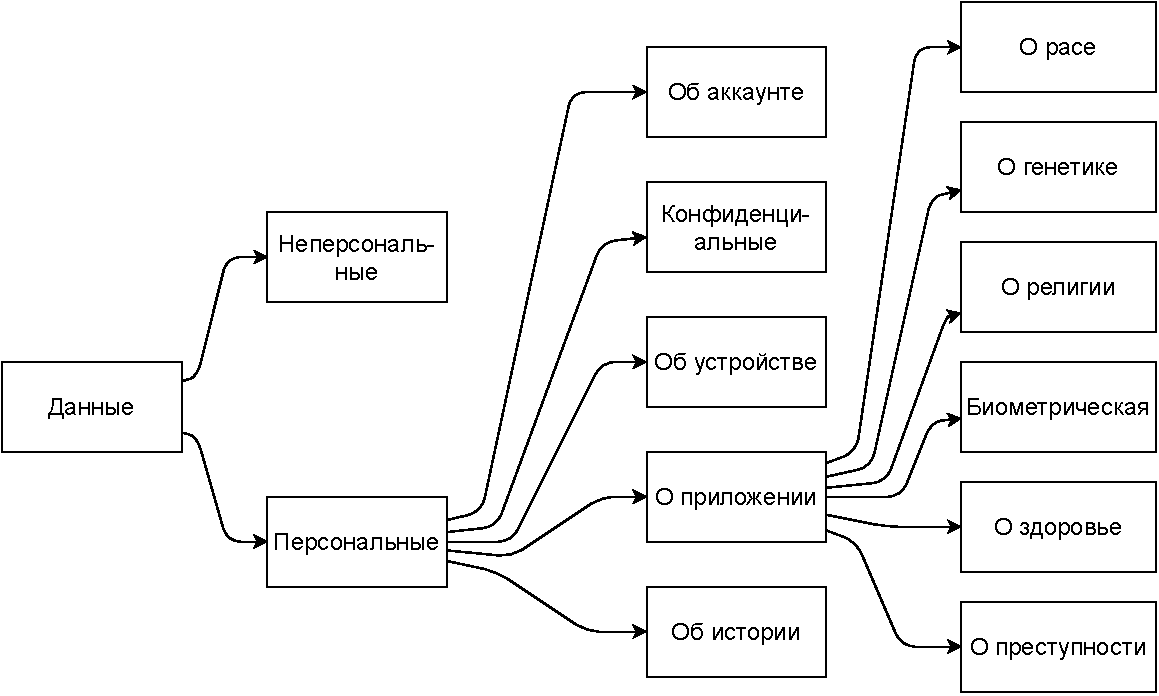
\includegraphics[width=.8\textwidth]{pics_mdpi1.pdf}}
    \vspace{-\baselineskip}
\end{figure}

Как следует из списка аспектов конфиденциальности использования персональных данных, некоторые аспекты напрямую связаны с обработкой данных, например сбор, обработка, совместное использование, хранение или безопасность данных, в то время как другие относятся к деятельности, которая косвенно связана с обработкой данных, например уведомления в случае изменения политики или нарушения данных, предоставление доступа, прав редактирования, удаления и т.д. По этой причине авторами были выделены два разных подкласса класса активности -- <<Действия с данными>> и <<Управление данными>>. На рисунке \ref{fig:figure4} показана иерархия подклассов <<Активность>>. 

\begin{figure}[H]
    \centering
    \ffigbox[\FBwidth]
    {\caption{Иерархия классов активности\label{fig:figure4}}}
    {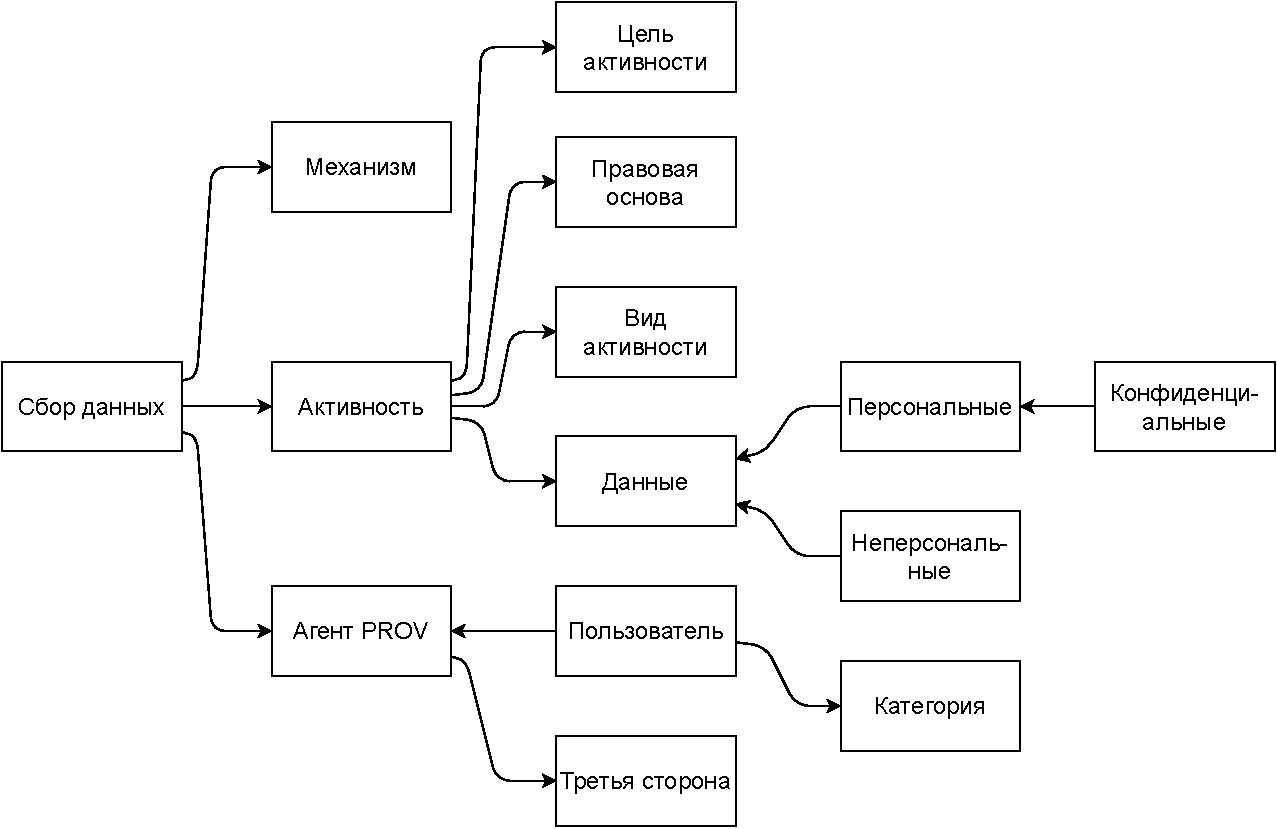
\includegraphics[width=.8\textwidth]{pics_mdpi2.pdf}}
    \vspace{-\baselineskip}
\end{figure}

Класс <<Активность>> -- это общий класс для определения различных типов операций по обработке данных. Несмотря на то, что эти действия имеют свои отличительные характеристики, можно выделить общие черты, такие как цель операций с данными, формат обрабатываемых данных -- анонимные или необработанные, правовая основа для обработки данных и контролирующие лица. На рисунке \ref{fig:figure5} показаны наиболее важные классы, относящиеся к деятельности по обработке данных. Цель обработки данных является важной концепцией при оценке рисков конфиденциальности, и авторы выделили следующие цели обработки данных: предоставление услуг, реклама и маркетинг, аналитика и исследования, персонализация, безопасность, слияние и поглощение, соответствие законодательству, другое и <<Не определено>>. Каждый из них представляет собой отдельный подкласс.

\begin{figure}[H]
    \centering
    \ffigbox[\FBwidth]
    {\caption{Контекст активности с данными\label{fig:figure5}}}
    {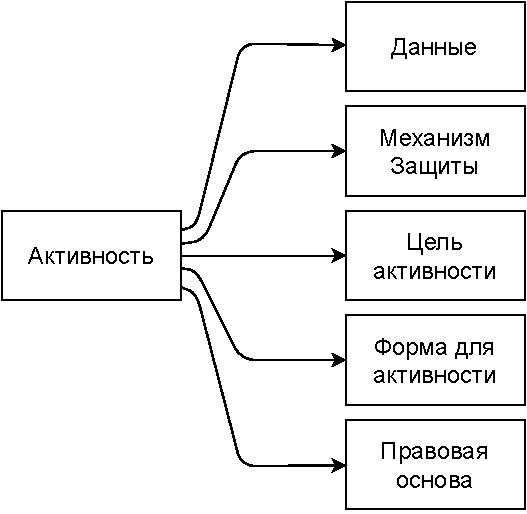
\includegraphics[width=.5\textwidth]{pics_mdpi3.pdf}}
    \vspace{-\baselineskip}
\end{figure}

Чтобы указать владельца данных, обработчика данных, а также других третьих сторон, участвующих в обработке данных, используется класс <<Агент>>. Авторы предлагают повторно использовать эту концепцию из онтологии PROV-O, которая определяет концепт <<Агент>> как субъект, который несет некоторую форму ответственности за происходящую деятельность, за наличие сущности или за деятельность другого агента \cite{MDPI22}. Эта концепция позволяет указать случаи, когда данные собираются от третьих сторон, таких как социальные сети, общедоступные источники с открытым исходным кодом. Класс <<Агент>> также используется для выявления случаев, когда данные собираются от посторонних лиц, то есть людей, которые не владеют устройством или услугой и с большой вероятностью не дают согласия на обработку данных.

Класс <<Механизм>> -- это общий класс, который используется для описания различных инструментов, опций, механизмов и интерфейсов, поддерживающих реализацию действий -- сбор данных, совместное использование, использование, уведомление в случае изменения политики или нарушения данных. Он используется для характеризации таких свойств, как режим обработки (автоматический или нет), детали реализации деятельности, такие как уведомление по электронной почте или на веб-сайте, доступ к данным через приложение или через конкретный запрос по почте и т.д.

Все упомянутые выше классы связаны друг с другом с помощью свойств, определяющих семантические отношения между ними.

Важно упомянуть, что в работе \cite{P2Onto} авторами предлагается методика оценивания рисков, базирующаяся на онтологическом представлении политик безопасности. Авторы \cite{P2Onto} считают, что эта онтология может служить основой для разработки интерактивных моделей визуализации на основе графов, нацеленных на объяснение рисков конфиденциальности для конечного пользователя в ясной и удобочитаемой форме. 

\subsection{Постановка задачи}
В связи с растущей актуальностью вопросов защиты персональных данных как никогда важными становятся методы формализации политик безопасности и оценивания рисков при согласии пользователя на передачу личных данных. Рассмотренные работы в данной области продемонстрировали возможность формализации политик безопасности, а также оценивания рисков при согласии с политикой конфиденциальности. Однако, пока не было предложено полностью автоматизированного решения для формализации политик безопасности и оценивания рисков. В связи с этим актуальна проблема автоматизации предложенных подходов. 

Таким образом задачей выпускной квалификационной работы является разработка методик и инструментов для сбора и аннотирования данных для поддержки системы формализации политик безопасности, которая в перспективе может быть использована при оценке рисков конфиденциальности.

\newpage
\section{Проектирование методики анализа политик безопасности}

\subsection{Исследование методов анализа текста на основе моделей, обучающихся без учителя}

Вопреки тенденциям на использование технологий машинного обучения для формализации политик безопасности, были сделаны попытки осуществить формализацию с помощью различных алгоритмов кластеризации.

Основанием для проведения данных экспериментов послужила особенность моделей построенных глубоком обучении -- необходимость наличия размеченной выборки данных для обучения. Сбор данных для этих целей -- трудоемкий процесс, равно как и аннотирование собранных данных.

Поэтому были протестированы различные алгоритмы кластеризации и тематического моделирования. Также была сделана попытка анализа политик безопасности на основе частеречной разметки и контекстно-свободных грамматик.

\subsubsection{Статистические модели текстовых документов}

В рамках экспериментов со строгими методами анализа текстов были протестированы две модели векторизованного представления текста -- Bag-of-Words и TF-IDF. Модель Bag-of-Words представляет документ в виде матрицы, представленной на рисунке \ref{fig:bow}. 

\begin{figure}[H]
    \centering
    \ffigbox[\FBwidth]
    {\caption{Bag-of-Words матрица\label{fig:bow}}}
    {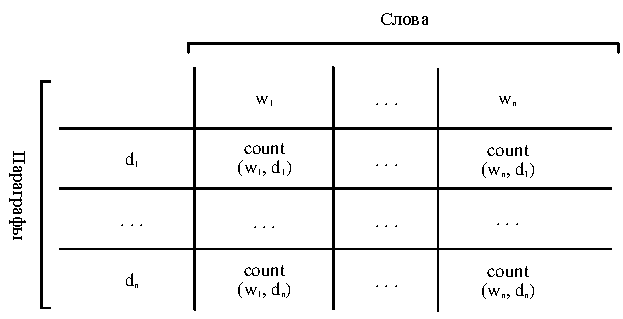
\includegraphics[width=.7\textwidth]{bow.pdf}}
    \vspace{-\baselineskip}
\end{figure}

Здесь слова каждого абзаца подсчитываются и сопоставляются с абзацами, в которых они встретились. Модель TF-IDF представляет документ в виде матрицы, представленной на рисунке \ref{fig:tfidf}. Формула (\ref{eq:tfidf}) показывает, как можно получить метрику TF-IDF.
\begin{equation}
    \label{eq:tfidf}
    tfidf(t, d, D) = \frac{n_t}{\displaystyle\sum_k n_k} \times 
    log \frac{ \big|{D}\big| }
    { \big|\left\{ d_i \in D : t \in d_i \right\}\big| },
\end{equation}
\makebox[1.25cm]{где\hfill}$t$ -- термин или слово,\\
\makebox[1.25cm]{}$d$ -- конкретный абзац,\\
\makebox[1.25cm]{}$D$ -- набор абзацев. 

Итак, модель TF-IDF придает больший вес словам которые использованы меньше раз. Это может быть полезно, когда тексты схожи с точки зрения используемых слов, как в случае с политиками безопасности \cite{LETI}.

\begin{figure}[H]
    \centering
    \ffigbox[\FBwidth]
    {\caption{Матрица TF-IDF\label{fig:tfidf}}}
    {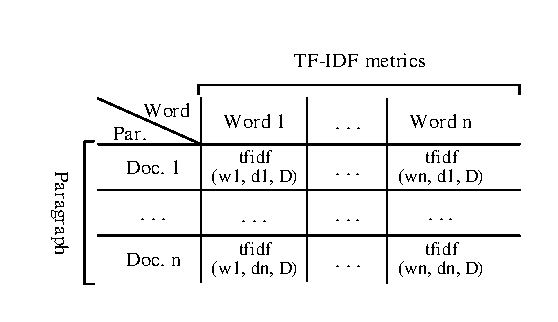
\includegraphics[width=.7\textwidth]{tfidf.pdf}}
    \vspace{-\baselineskip}
\end{figure}

\subsubsection{Подход основанный на латентно-семантическом анализе текста}

Современные методы кластеризации текстов позволяют определять тематику текстов с высокой точностью. Однако, большинство из этих методов принимают тексты с самыми разными темами как вход для алгоритмов. Тексты со схожими тематиками можно проанализировать с помощью ла\-тен\-тно-семантического анализа дважды: группировать тексты по темам один раз, и предоставить еще более детальное разделение их по подтемам во второй раз. Такой подход можно использовать для более точной классификации абзацев с точки зрения их характеристик и аспектов использования персональных данных. Следует отметить, что латентно-семантический поиск сильно зависит от глобального текстового контекста с потерями информации о локальных контекстных отношениях между словами. Были выделены девять тем конфиденциальности, которые следует сопоставить с абзацами согласия пользователя сайта -- <<Сбор личных данных>>, <<Сбор данных третьими лицами>>, <<Управление личными данными>>, <<Механизмы защиты персональных данных>> и другие. Очевидно, что аспекты обращения с данными состоят из нескольких слов, и в некоторых случаях перекрываются. На основании этих фактов была выдвинута гипотеза о том, что латентно-семантический поиск способен обнаружить даже незначительную разницу в тексте абзацев при пропуске частых слов. Перед применением латентно-семантического анализа требуется предварительная обработка входных данных. Обычно эта процедура включает в себя очистку данных, удаление гиперссылок, пунктуации и т.д. Также текст политик конфиденциальности был разбит на массив абзацев. Каждый абзац был преобразован в массив слов, которые он содержит. Следующим шагом было удаление наиболее частых, но не столь значимых слов, так называемых стоп-слов. Наконец была применена операция стемминга, чтобы рассматривать только основную часть всех слов полученных от единого корня.

Пусть A -- это матрица абзацев и слов, тогда формула (\ref{eq:lsa}) будет следующей:

\newpage
\begin{equation}
    \label{eq:lsa}
    A = U \times S \times V^T,
\end{equation}
\makebox[1.25cm]{где\hfill}$A$ -- матрица слов и параграфов;\\
\makebox[1.25cm]{\hfill}$U$ -- ортонормированная матрица $U$;\\
\makebox[1.25cm]{\hfill}$V$ -- ортонормированная матрица $V$;\\
\makebox[1.25cm]{\hfill}$S$ -- диагональная матрица $S$, значения которой сингулярны для $A$.

После того, как матрица была разделена на три компоненты, матрица $U$ содержит $n$-мерные векторы, которые можно интерпретировать как координаты в $n$-мерном пространстве \cite{LSA}. Документы могут быть распределены по кластерам по значениям этих координат. Проведенные эксперименты с латентно-семантическим анализом выполнялись с использованием набора данных с открытым исходным кодом, который включает 115 политик безопасности, которые были размечены вручную, и все абзацы присвоены одному или нескольким сценариям использования персональных данных \cite{MDPI18}. Результаты экспериментов для модели Bag-of-Words представлены в таблице \ref{tab:clusters1}, в ней показаны полученные кластеры и соответствующие значения координат.

\begin{ltwrap}{2mm}{1}{\footnotesize}
    \begin{longtable}[H]{|C{.05\x}|M{.2\x}|M{.2\x}|M{.2\x}|M{.2\x}|}
        \caption{Кластеры политик безопасности для модели Bag-of-Words\label{tab:clusters1}}\\\hline
        \multicolumn{1}{|H{.05\x}|}{№}
        & \multicolumn{1}{H{.2\x}|}{Координата 1} 
        & \multicolumn{1}{H{.2\x}|}{Координата 2} 
        & \multicolumn{1}{H{.2\x}|}{Координата 3} 
        & \multicolumn{1}{H{.2\x}|}{Координата 4}\\\hline
        \endfirsthead
        \caption*{Продолжение таблицы \ref{tab:clusters1}}\\\hline
        \multicolumn{1}{|H{.05\x}|}{№}
        & \multicolumn{1}{H{.2\x}|}{Координата 1} 
        & \multicolumn{1}{H{.2\x}|}{Координата 2} 
        & \multicolumn{1}{H{.2\x}|}{Координата 3} 
        & \multicolumn{1}{H{.2\x}|}{Координата 4}\\\hline
        \endhead
        \endfoot
        \endlastfoot
        0 & 0.634 inform  & 0.280 may        & 0.276 use     & 0.232 servic   \\\hline
        1 & 0.202 cooki   & 0.466 inform    & 0.336 site    & 0.257 use      \\\hline
        2 & 0.524 privaci & 0.433 polici    & 0.388 cooki   & 0.219 site     \\\hline
        3 & -0.589 servic & 0.344 site      & 0.244 parti   & -0.240 third   \\\hline
        4 & -0.504 parti  & 0.486 third    & -0.449 servic & 0.235 advertis \\\hline
        5 & -0.594 site   & 0.278 cooki     & 0.272 websit  & 0.264 privaci  \\\hline
        6 & -0.326 may    & 0.311 site      & 0.307 servic  & -0.293 email   \\\hline
        7 & -0.437 may    & -0.369 advertis & 0.345 person  & 0.319 cooki    \\\hline
        8 & 0.501 may     & -0.315 email    & -0.281 use    & -0.264 address \\\hline
        9 & -0.488 user   & -0.384 use      & 0.310 provid  & -0.301 websit  \\\hline
    \end{longtable}
\end{ltwrap}

Как видно, результаты противоречивы, поэтому трудно понять, какая из тем каким смыслом обладает. Затем рассчитывалась метрика принадлежности к теме с помощью библиотеки Gensim \cite{Gensim} и результаты снова не были обнадеживающими. Результаты расчета метрики принадлежности кластеру представлены в таблице \ref{tab:affiliation_bow1}.

\begin{ltwrap}{2mm}{1}{\footnotesize}
    \begin{longtable}[H]{|H{.13\x}|C{.1\x}|C{.1\x}|C{.1\x}|C{.1\x}|C{.1\x}|}
        \caption{Принадлежность кластерам\label{tab:affiliation_bow1}}\\\hline
        \endfirsthead
        \caption*{Продолжение таблицы \ref{tab:clusters1}}\\\hline
        \endhead
        \endfoot
        \endlastfoot
        Topic       & 0     & 1     & 2    & 3     & 4     \\\hline
        Affiliation & 2.27  & -0.8  & 0.15 & -0.22 & -1.2  \\\hline
        Topic       & 5     & 6     & 7    & 8     & 9     \\\hline
        Affiliation & -0.17 & -0.15 & -0.2 & 0.22  & -0.07 \\\hline
    \end{longtable}
\end{ltwrap}

Другие результаты с параграфами, относящимися к другому аспекту обращения с данными, были почти такими же. Результаты
представлены в таблице \ref{tab:affiliation_bow2}.

\begin{ltwrap}{2mm}{1}{\footnotesize}
    \begin{longtable}[H]{|H{.13\x}|C{.1\x}|C{.1\x}|C{.1\x}|C{.1\x}|C{.1\x}|}
        \caption{Принадлежность кластерам\label{tab:affiliation_bow2}}\\\hline
        \endfirsthead
        \caption*{Продолжение таблицы \ref{tab:clusters1}}\\\hline
        \endhead
        \endfoot
        \endlastfoot
        Topic       & 0    & 1     & 2    & 3    & 4    \\\hline
        Affiliation & 2.59 & -0.76 & 0.64 & 0.74 & 0.13 \\\hline
        Topic       & 5    & 6     & 7    & 8    & 9    \\\hline
        Affiliation & 0.14 & -0.12 & 0.23 & 0.12 & 0.41 \\\hline
    \end{longtable}
\end{ltwrap}

Все протестированные абзацы были сопоставлены с кластером 0, что не может быть верным так как абзацы относились к заведомо разным аспектам обращения с персональными данными. 

Результаты экспериментов для модели TF-IDF представлены далее, в таблице \ref{tab:clusters2}. Также показывались десять кластеров и координаты в семантическом пространстве. И, как в первом случае с <<мешком слов>>, по значениям координат невозможно судить о теме кластера.

\begin{ltwrap}{2mm}{1}{\footnotesize}
    \begin{longtable}[H]{|C{.05\x}|M{.2\x}|M{.2\x}|M{.2\x}|M{.2\x}|}
        \caption{Кластеры политик безопасности для модели TF-IDF\label{tab:clusters2}}\\\hline
        \multicolumn{1}{|H{.05\x}|}{№}
        & \multicolumn{1}{H{.2\x}|}{Координата 1} 
        & \multicolumn{1}{H{.2\x}|}{Координата 2} 
        & \multicolumn{1}{H{.2\x}|}{Координата 3} 
        & \multicolumn{1}{H{.2\x}|}{Координата 4}\\\hline
        \endfirsthead
        \caption*{Продолжение таблицы \ref{tab:clusters2}}\\\hline
        \multicolumn{1}{|H{.05\x}|}{№}
        & \multicolumn{1}{H{.2\x}|}{Координата 1} 
        & \multicolumn{1}{H{.2\x}|}{Координата 2} 
        & \multicolumn{1}{H{.2\x}|}{Координата 3} 
        & \multicolumn{1}{H{.2\x}|}{Координата 4}\\\hline
        \endhead
        \endfoot
        \endlastfoot
        0 & 0.202 cooki     & 0.2 may        & 0.198 inform   & 0.198 site     \\\hline
        1 & 0.573 cooki     & 0.262 browser  & 0.195 advertis & 0.182 web      \\\hline
        2 & -0.406 media    & 0.291 cooki    & 0.282 health   & 0.279 advertis \\\hline
        3 & -0.453 health   & 0.258 email    & -0.204 kaleida & 0.191 address  \\\hline
        4 & 0.423 health    & 0.215 media    & 0.205 kaleida  & -0.199 secur   \\\hline
        5 & -0.299 advertis & 0.262 health   & -0.252 media   & -0.213 privaci \\\hline
        6 & -0.325 media    & 0.263 polici   & 0.249 privaci  & 0.197 chang    \\\hline
        7 & 0.280 cooki     & -0.216 device  & -0.183 health  & -0.166 social  \\\hline
        8 & -0.223 advertis & -0.206 teenag  & -0.206 inelig  & 0.176 child    \\\hline
        9 & -0.263  child   & -0.26 wireless & 0.245 message  & 0.239 parent   \\\hline
    \end{longtable}
\end{ltwrap}

Результаты кластеризации снова противоречивы, поэтому трудно сказать, какая конкретная тема какой аспект политики конфиденциальности описывает. В разных темах встречаются одни и те же слова с изменением веса. Для искомых аспектов политики конфиденциальности нет тем, которые могли бы их точно описать. Затем с помощью библиотеки Gensim был рассчитан показатель принадлежности к теме, и результаты снова не были обнадеживающими. Результаты расчета аффилиации абзаца одной из политик конфиденциальности к полученным кластерам представлены в таблице \ref{tab:affiliation_tfidf1}.

\begin{ltwrap}{2mm}{1}{\footnotesize}
    \begin{longtable}[H]{|H{.13\x}|C{.1\x}|C{.1\x}|C{.1\x}|C{.1\x}|C{.1\x}|}
        \caption{Принадлежность кластерам\label{tab:affiliation_tfidf1}}\\\hline
        \endfirsthead
        \caption*{Продолжение таблицы \ref{tab:affiliation_tfidf1}}\\\hline
        \endhead
        \endfoot
        \endlastfoot
        Topic       & 0    & 1     & 2     & 3     & 4     \\\hline
        Affiliation & 2.18 & -0.97 & -0.69 & -0.27 & 0.65  \\\hline
        Topic       & 5    & 6     & 7     & 8     & 9     \\\hline
        Affiliation & 0.98 & -1.17 & 0.8   & 0.27  & 0.01  \\\hline
    \end{longtable}
\end{ltwrap}

Результат для другого абзаца, относящегося к другой политике конфиденциальности, был почти такой же. Результаты представлены в таблице \ref{tab:affiliation_tfidf2}.

\begin{ltwrap}{2mm}{1}{\footnotesize}
    \begin{longtable}[H]{|H{.13\x}|C{.1\x}|C{.1\x}|C{.1\x}|C{.1\x}|C{.1\x}|}
        \caption{Принадлежность кластерам\label{tab:affiliation_tfidf2}}\\\hline
        \endfirsthead
        \caption*{Продолжение таблицы \ref{tab:affiliation_tfidf2}}\\\hline
        \endhead
        \endfoot
        \endlastfoot
        Topic       & 0    & 1    & 2     & 3     & 4     \\\hline
        Affiliation & 1.82 & 0.25 & 0.49  & 0.29  & -0.04 \\\hline
        Topic       & 5    & 6    & 7     & 8     & 9     \\\hline
        Affiliation & 0.74 & 0.52 & -0.04 & -0.58 & -1.33 \\\hline
    \end{longtable}
\end{ltwrap}

Как можно заметить, результаты для модели TF-IDF аналогичны результатам модели Bag-of-Words, за исключением нескольких незначительных изменений. Все абзацы снова были сопоставлены с кластером 0, что неверно, потому что они на самом деле описывают разные сценарии использования персональных данных. Эти эксперименты позволили сделать вывод, что использование латентно-семантического анализа не дает ценной информации о содержании онлайн-согласия пользователя. Проблема может быть связана с тем, что сценарии использования персональных данных очень похожи между собой, и для того, чтобы различать разные сценарии необходимо учитывать локальный контекст.

В результате апробации алгоритма латентно-семантического анализа было выяснено, что для кластеризации экстремально схожих между собой текстов он подходит не лучшим образом \cite{LETI}.

\subsubsection{Подход основанный на латентном размещении Дирихле}

Для тестирования латентного размещения Дирихле был как и ранне выбран датасет OPP-115 с открытым исходным кодом \cite{MDPI18}. В большинстве случаев аспекты относятся к абзацам текста, а некоторые абзацы относятся к нескольким категориям одновременно. На рисунке \ref{fig:opp1} показано распределение абзацев по категориям. Хорошо видно, что есть две основные категории – <<Third-party Sharing/Collection>> и <<First-party Collection and Use>>, которые преобладают над остальными.

Чтобы применить LDA к анализу политики конфиденциальности, тексты политик конфиденциальности были разбиты на набор абзацев. Каждый абзац был преобразован в массив слов, а затем удалены наиболее частые, но не значащие слова, так называемые стоп-слова. Также была выполнена лемматизация, чтобы обобщить некоторые слова, для получения более точных результатов.

В ходе экспериментов как и раннее были протестированы две модели векторизации текста – Bag-of-Words и TF-IDF, и оказалось, что метрика TF-IDF предоставляет более подробную информацию о сценариях использования данных, поскольку эта модель векторизации дает более высокие веса словам, которые реже используются.

\begin{figure}[H]
    \centering
    \ffigbox[\FBwidth]
    {\caption{Распределение по сценариям использования данных\label{fig:opp1}}}
    {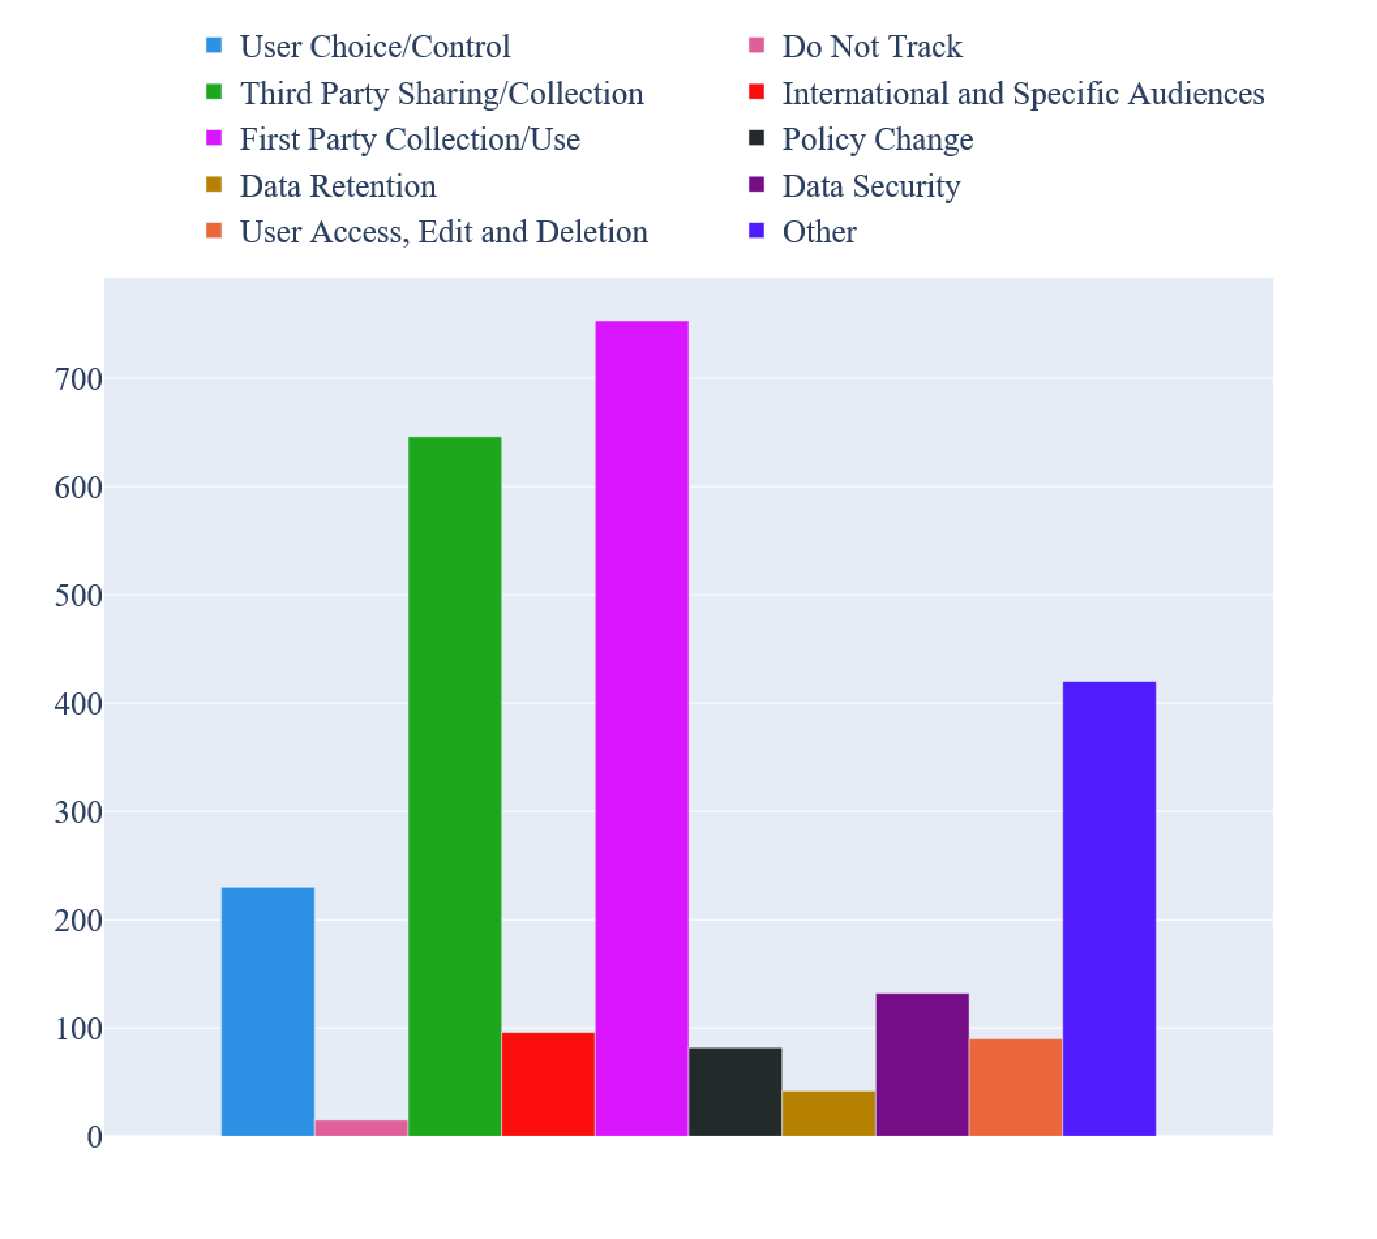
\includegraphics[width=.75\textwidth]{last1.pdf}}
    \vspace{-\baselineskip}
\end{figure}

Оптимальное количество кластеров, то есть семантических моделей, было определено как 15, поскольку такое значение соответствует максимальному значению когерентности, рассчитанному с помощью библиотеки Gensim \cite{MDPI13}. Важно отметить, что это число отличается от числа категорий, обозначенных создателями набора данных OPP-115.

Результаты экспериментов для модели TF-IDF показаны в таблице \ref{tab:advanced_modeling}. В таблице \ref{tab:advanced_modeling} приведен список координат, которые формируют семантические модели тем. Координаты используются для составления гипотезы об использовании личных данных и сценариях их применения.

Хорошо видно, что большинство извлеченных моделей посвящено сценариям <<First-Party Collection and Use>> и <<Third-Party Sharing/Collection>>. Это полностью соответствует распределению категорий в наборе данных. Абзацы различаются характеристиками семантических моделей. Например, тематическая модель 9 раскрывает варианты согласия/отказа при обмене личными данными в рекламных целях, тематическая модель 6 посвящена использованию файлов cookie первыми и третьими сторонами, некоторые тематические модели предоставляют информацию о типах собираемых личных данных: информация об учетной записи пользователя (тематическая модель 7), финансовые данные (тематическая модель 2), данные отслеживания местоположения и аналитики (тематическая модель 11). Некоторые темы, такие как тематические модели 4 и 10, раскрывают довольно специфические аспекты использования личных данных, такие как безопасность данных, включая случай, когда данные передаются третьим лицам, и уведомление в случае изменения политики. Некоторые тематические модели являются довольно общими, например, модели характеризуют очень общие проблемы, связанные со сбором данных первой стороной и сторонним совместным использованием 0,1 и 3.

\begin{ltwrap}{2mm}{1}{\footnotesize}
    \begin{longtable}[H]{|C{.05\x}|M{.475\x}|M{.475\x}|}
        \caption{Тематическое моделирование\label{tab:advanced_modeling}}\\\hline
        \multicolumn{1}{|H{.05\x}|}{№}
        & \multicolumn{1}{H{.475\x}|}{Координаты семантического пространства} 
        & \multicolumn{1}{H{.475\x}|}{Возможные сценарии использования}\\\hline
        \endfirsthead
        \caption*{Продолжение таблицы \ref{tab:advanced_modeling}}\\\hline
        \multicolumn{1}{|H{.05\x}|}{№}
        & \multicolumn{1}{H{.475\x}|}{Координаты семантического пространства} 
        & \multicolumn{1}{H{.475\x}|}{Возможные сценарии использования}\\\hline
        \endhead
        \endfoot
        \endlastfoot
        0 & service, friend, story, child, cookie, use, product, email, compromised, card & First-party collection \& usage (usage of cookies, e-mail), Special audience (children) \\\hline
        1 & schedule, channel, analytic, happy, website, gather, address, mingle, moreover, identifiable & First-party collection (identifiable user data) \\\hline
        2 & collect, credit, card, us, address, pursuant, email, service, personal, may & First-party collection: payment credentials \\\hline
        3 & state, united, asset, website, policy, personal, privacy, party, third, sm & Third-party sharing \\\hline
        4 & security, personal, rating, site, u, disclosure, service, policy, physical, third & Data security (including third-party sharing)  \\\hline
        5 & party, third, child, service, cookie, personal, personally, site, company, identifiable & Third-party sharing (usage of cookies) \\\hline
        6 & service, website, personal, site, cookie, party, third, data, use, us & First-party collection \& Third-party sharing (for: services provision, usage of website data and cookies) \\\hline
        7 & personal, service, account, information, site, device, u, may, provide, use & First-party collection: user account information \\\hline
        8 & device, resume, message, policy, privacy, social, service, site, website, networking & Other \\\hline
        9 & opt, collect, site, third, advertising, personal, party, service, u, privacy & First-party collection \& Opt-in, opt-out for advertising \\\hline
        10 & military, change, policy, time, site, web, page, privacy, cookie, post & Privacy policy change, including notification mechanism \\\hline
        11 & navigating, service, google, non, adsense, nielsen, account, collect, device, privacy & First-party collection: device and location information \\\hline
        12 & station, feedback, service, consented, java, script, merchant, cookie, child, st & Other \\\hline
        13 & cookie, service, third, party, site, website, california, flash, use, technology & Third-party sharing \& Special audience: California residents \\\hline
        14 & child, forum, trade, age, pii, conversation, chat, branded, personal & Special audience: children \\\hline
    \end{longtable}
\end{ltwrap}

Однако необходимо учитывать, что политики конфиденциальности в большинстве случаев являются очень общими и неструктурированными, они не содержат четкой спецификации действий по обработке данных. Для некоторых тематических моделей было сложно определить аспекты сценариев использования, они были объединены в группу <<Other>>.

Также стоит отметить, что не было выявлено моделей, посвященных хранению данных и аспектам доступа, редактирования и удаления данных. Это могло произойти из-за того, что количество абзацев, содержащих эту информацию, невелико, и они семантически довольно близки к сценарию <<First-Party Collection and Use>>. Напротив, были найдены темы посвященные аспектам <<International and Special Audience>>, <<Data Security>> и <<Privacy Policy Change>>, хотя количество их вхождений в наборе данных сопоставимо с <<Data Retention>> и <<User Access, Edit and Deletion>>.

Используя извлеченные тематические модели, было проанализировано содержание политик конфиденциальности и вручную оценена точность кластеризации абзацев для набора выбранных политик. Например, для политики конфиденциальности Xiaomi \cite{MDPI14} была получена точность 69\%. На рисунке \ref{fig:opp2} показано распределение семантических тематических моделей абзацев в тексте политики конфиденциальности Xiaomi. 

\begin{figure}[H]
    \centering
    \ffigbox[\FBwidth]
    {\caption{Распределение по сценариям использования данных, полученное с помощью LDA\label{fig:opp2}}}
    {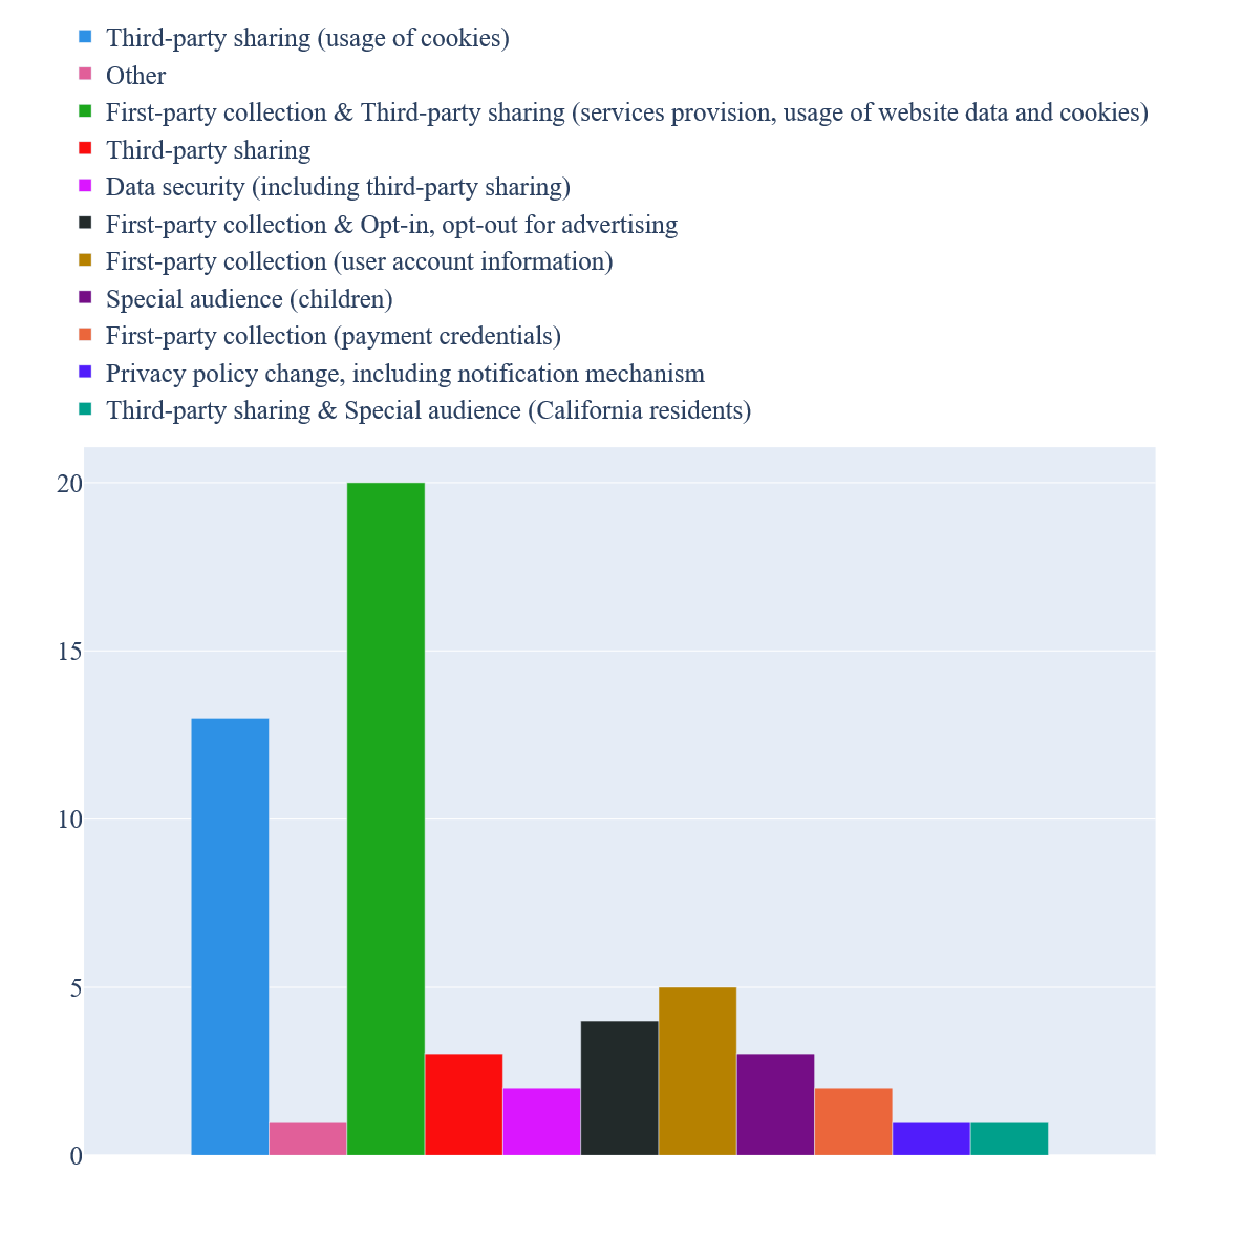
\includegraphics[width=.75\textwidth]{last2.pdf}}
    \vspace{-\baselineskip}
\end{figure}

Отчетливо видно, что большая часть документа посвящена описанию различных аспектов <<First-Party Collection and Use>> – указанию, какие типы данных собираются, есть ли какие-либо варианты выбора/отказа. Полученные результаты также сравнивались с результатами \cite{MDPI7} с помощью онлайн-инструмента Pribot \cite{Polisis}. Сравнительный анализ показал, что LDA выявило все основные аспекты использования персональных данных, за исключением одной целевой детской аудитории. Когда была перепроверена политика Xiaomi, выяснилось, что данному аспекту было посвящено лишь одно предложение.

\subsubsection{Подход основанный на применении контекстно-свободных грамматик и синонимическом поиске}

Другой предложенный подход -- подход, основанный на анализе с помощью контекстно-свободных грамматик и синонимического поиска. Синонимический поиск в данном случае -- это подмена ключевых слов и их синонимов метками, например <<\_\_FP\_A\_\_>> означает, что это слово и его синонимы считаются акторами (первым лицом). Этот метод можно применить ко многим другим концепциям. Например, сообщения электронной почты, аватары, местоположение также могут быть объектами и синонимами абстрактной метки <<\_\_CN\_\_>>, которая означает существительное сбора или объект сбора. Так все ключевые слова могут быть преобразованы в их смыслы в контексте предметной области. Маркировка выполняется просто, все слова, совпадающие с пулами, заменяются метками этих пулов.

Предварительная обработка данных в данном случае состоит из токенизации и лемматизации для более гибкой замены слов на метки их пулов.

При анализе пользовательского согласия сайта недостаточно найти ключевые слова, относящиеся к разным типам персональных данных, например цель и правовую основу распознать гораздо сложнее. Следующий шаг -- установить отношения между словами в предложениях, чтобы можно было определенно сказать, что ярлыки пулов синонимов связаны друг с другом и формируют логическая цепочку. Один из возможных способов определения отношений слов в тексте на естественном языке -- это синтаксический анализ предложения, основанный на частеречной разметке \cite{POS}. Имея размеченное по частям речи предложение, парсер грамматики NLTK \cite{NLTK} строит деревья предложений по правилам грамматики. Одно из таких деревьев в обозначениях NLTK можно увидеть на рисунке \ref{fig:nltk_tree} \cite{NLTK}.

\begin{figure}[H]
    \centering
    \ffigbox[\FBwidth]
    {\caption{Пример грамматического разбора\label{fig:nltk_tree}}}
    {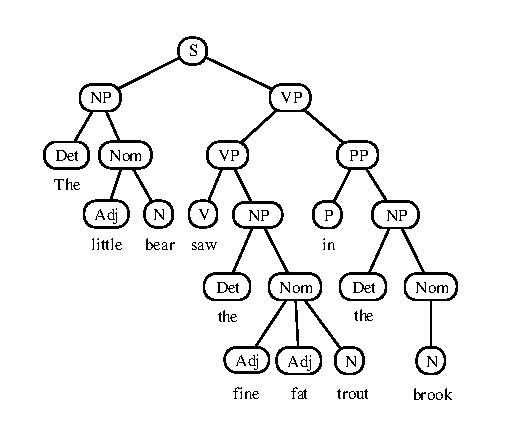
\includegraphics[width=.7\textwidth]{tree.pdf}}
    \vspace{-\baselineskip}
\end{figure}

Здесь <<S>> -- основа предложения, <<NP>> -- именная фраза, <<VP>> -- глагольная фраза, <<Adj>> -- прилагательное, <<Nom>> -- именное словосочетание, <<PP>> -- предлог фраза, <<Det>> -- артикль, <<V>> -- глагол, <<N>> -- существительное, <<P>> -- предлог.

В предлагаемом подходе немного другая грамматическая запись. Созданная грамматика представлена в (\ref{eq:grammar1}). 

\begin{equation}
    \label{eq:grammar1}
    \left\{ 
        \begin{array}{l}
            D \rightarrow S\ |\ S\ D\ |\ S\ U\ D\ \\
            S \rightarrow NPG\ \ \ VBG \\
            VPG \rightarrow VP\ |\ VP\ \ VPG\ |\ VP\ \ U\ \ VPG \\
            NPG \rightarrow NP\ |\ NP\ \ NPG\ |\ NP\ \ U\ \ NPG \\
            AJPG \rightarrow AJ\ |\ AJ\ \ APG\ |\ AJ\ \ U\ \ APG \\
            AVPG \rightarrow AV\ |\ AV\ \ APG\ |\ AV\ \ U\ \ APG \\
            VP \rightarrow V \ \ APG\ |\ V\ \ PPG\ |\ V\ \ PP\ \ APG \\
            NP \rightarrow NOM\ |\ DET\ \ NOM \\
            NOM \rightarrow N\ |\ AJPG\ \ N \\
            PP \rightarrow NPG\ |\ P\ \ NPG
        \end{array}
    \right.,
\end{equation}
\makebox[1.25cm]{где\hfill}$D$ -- документ,\\
\makebox[1.25cm]{}$SB$ -- синтаксическая основа предложения с его зависимостями,\\
\makebox[1.25cm]{}$U$ -- союз,\\
\makebox[1.25cm]{}$NPG$ -- группа именных фраз,\\
\makebox[1.25cm]{}$VPG$ -- группа глагольных фраз,\\
\makebox[1.25cm]{}$AJPG$ -- группа однородных прилагательных,\\
\makebox[1.25cm]{}$AVPG$ -- группа однородных наречий,\\
\makebox[1.25cm]{}$PPG$ -- группа однородных дополнений,\\
\makebox[1.25cm]{}$VP$ -- глагольная группа,\\
\makebox[1.25cm]{}$NP$ -- именная группа,\\
\makebox[1.25cm]{}$NOM$ -- номинальная группа,\\
\makebox[1.25cm]{}$P$ -- предлог,\\
\makebox[1.25cm]{}$AJ$ -- прилагательное,\\
\makebox[1.25cm]{}$AV$ -- наречие,\\
\makebox[1.25cm]{}$PP$ -- существительное с предлогом,\\
\makebox[1.25cm]{}$N$ -- существительное,\\
\makebox[1.25cm]{}$V$ -- глагол,\\
\makebox[1.25cm]{}$DET$ -- определяющее слово.

Грамматика из формулы (\ref{eq:grammar1}) позволяет рекурсивно выделять основу предложения и последовательности глагола, существительного, прилагательного, наречия и т.д. Это все еще не идеальное решение, но способное обрабатывать довольно сложные предложения в политиках безопасности. Этот подход требует использования пулов синонимов, которые соответствуют различным ключевым словам. Поэтому в грамматику включены метки пулов синонимов, привязанных к части речи. Метки пулов вручную назначены частям речи для связи их с нотацией частей речи NLTK, это показано в формуле (\ref{eq:grammar2}).
\begin{equation}
    \label{eq:grammar2}
    \left\{ 
        \begin{array}{l}
            U \rightarrow NLTK\_CC \\
            DET \rightarrow NLTK\_DT \\
            AJ \rightarrow NLTK\_JJ \\
            AV \rightarrow NLTK\_RB \\
            N \rightarrow \_\_CN\_\_\ |\ \_\_FP\_A\_\_\ |\ \_\_TP\_A\_\_\ |\ NLTK\_N \\
            V \rightarrow \_\_CV\_\_\ |\ NLTK\_V
        \end{array},
    \right. 
\end{equation}
\makebox[1.25cm]{где\hfill}$NLTK\_CC$ -- соединение NLTK,\\
\makebox[1.25cm]{}$NLTK\_N$ -- все формы существительных NLTK,\\
\makebox[1.25cm]{}$NLTK\_В$ -- все формы глаголов NLTK,\\
\makebox[1.25cm]{}$NLTK\_DET$ -- определители NLTK,\\
\makebox[1.25cm]{}$NLTK\_RB$ -- все формы наречий NLTK,\\
\makebox[1.25cm]{}$\_\_FP\_A\_\_$ -- метка актора-обладателя персональных данных,\\
\makebox[1.25cm]{}$\_\_TP\_A\_\_$ -- третья сторона,\\
\makebox[1.25cm]{}$\_\_CV\_\_$ -- глагол сбора,\\
\makebox[1.25cm]{}$\_\_CN\_\_$ -- существительное сбора.

Теги, начинающиеся с подчеркивания, являются метками пулов синонимов. Синтаксический анализ выполняет библиотека NLTK. На основе предложенной грамматики, описанной (\ref{eq:grammar1}) и (\ref{eq:grammar2}) и меток пулов было построено дерево тестового предложения, результат на рисунке \ref{fig:tree}.

Когда было построено дерево предложений, последовательность меток ключевых слов может быть распознана. В этом случае представленная на рисунке \ref{fig:tree}, последовательность <<\_\_FP\_A\_\_>>, <<\_\_CV\_\_>>, <<\_\_CN\_\_>> хорошо видна.

\begin{figure}[H]
    \centering
    \ffigbox[\FBwidth]
    {\caption{Дерево грамматического разбора\label{fig:tree}}}
    {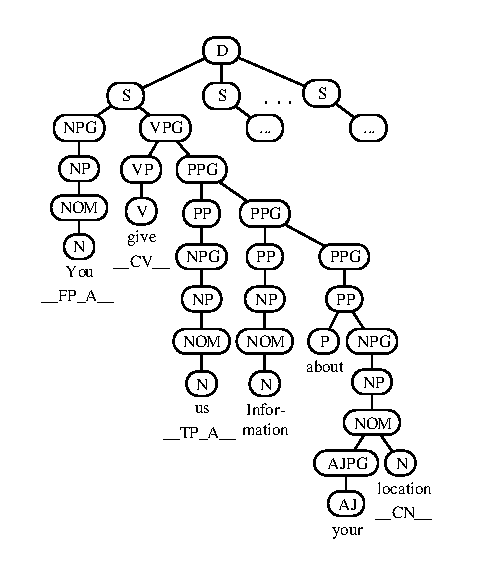
\includegraphics[width=.7\textwidth]{labeled_tree.pdf}}
    \vspace{-\baselineskip}
\end{figure}

Такие простейшие последовательности, раскрывают значения частей предложения и могут быть объединены в список, после этого весь смысл документов будет описан этим списком. Сочетание маркировки ключевых слов и синтаксического анализа дает значения ключевых слов с отношениями между этими словами, определенными в виде древовидных структур. Дерево структура данных более гибкая, чем строка предложения, деревья и особенно поддеревья показывают важные отношения между словами. Запросы к таким структурам могут дать необходимую информацию для построения логических последовательностей действующих лиц, их действий, субъектов этих действий и, наконец, обстоятельств. Предлагаемый подход определенно имеет такие недостатки, как низкая производительность, вручную определенные пулы синонимов и т.д. \cite{LETI}.

\subsubsection{Выводы методам анализа текста на основе моделей, обучающихся без учителя}

Эксперименты показали, что оба рассмотренных метода имеют как преимущества, так и определенные недостатки. Хотя предложенные подходы, оказались противоречивыми, окончательные результаты заслуживают внимания. Подход с латентно-семантическим поиском оказался не слишком эффективным. Однако, подход основанный на грамматическом анализе предложений и синонимическом поиске дал определенные результаты. Хоть он и не является производительным, с его помощью возможно производить выделение логических цепочек из предложений для получения более формального описания политик безопасности нежели их текстовые варианты. Алгоритм LDA показал наилучшие результаты, однако этих результатов все же не достаточно для выявления таких тонких сущностей как аттрибуты классов, представленных в онтологии из работы \cite{P2Onto}.

Исходя из проведенных исследований стало понятно, что более предпочтительным вариантом решения задачи будет подход с применением моделей глубокого обучения. Реализация подобного проекта -- комплексная задача, ее можно разделить на несколько этапов. Сначала необходимо собрать датасет, потом разметить его для обучения модели, далее обучить модель и получить результаты. Однако, сбор датасета тоже является непростой задачей. Необходимость сбора нового датасета обусловлена еще и принятием GDPR в качестве основного документа, регулирующего обработку, хранение и использование персональных данных, в то время как существующие датасеты состоят из устаревших документов. Для того, чтобы осуществить сбор датасета необходим инструмент для поиска и скачивания веб-страниц из сети Интернет. Затем необходимо произвести очистку данных, удалить все теги со страниц, чтобы можно было передать текст аннотаторам. Все этапы сбора датасета полагаются на базу данных. Она лишена сложного объектно-реляционного моделирования, так как в ней по сути необходимо только хранить промежуточные результаты обработки текстовых материалов.

\subsection{Требования к программным компонентам, реализующим разработанную методику}

\subsubsection{Скрейпер веб-страниц}
Скачивание веб-страниц будет производиться инструментом, написанным на языке Python, с помощью библиотек можно скачивать страницы, анализировать данные содержащиеся в них, переходить по гиперссылкам и много другое. Такой инструмент позволит просматривать и сохранять содержимое страниц в автоматическом режиме без вмешательства пользователя. Таким образом, в автоматическом режиме можно сохранить и проанализировать огромное количество текстовой информации.

\subsubsection{Очистка скачанных страниц политик}
Для очистки страниц от кода разметки планируется использовать библиотеку html-sanitizer. Очистка кода необходима для того, чтобы аннотаторы могли максимально сфокусироваться на анализе текста, таким образом, получая чистый текст, они не будут отвлекаться на не имеющие значения в контексте задачи фрагменты.

\subsubsection{Инструмент разметки датасета}
Инструмент разметки датасета планируется реализовать с помощью веб-технологий. Серверная часть будет полагаться на приложение, написанное на языке PHP, которое будет регулировать порядок выдачи текста на аннотирование. Процесс разметки высокодинамичен, поэтому невозможно избежать написания качественной клиентской части приложения на языке javascript. Это позволит сделать работу аннотаторов максимально производительной, в одну сессию (страница не будет перезагружаться).

\subsubsection{Фреймворки глубокого обучения}
Аннотированный датасет должен быть легко адаптируемым для создания и тренировки модели анализа текста с использованием современных фреймворков машинного обучения, таких как Keras, PyTorch и другие. Они позволят быстро создавать классификаторы самых разных конфигураций и типов.

После того как классификатор будет сконфигурирован, останется лишь обучить его на датасете, полученном ранее.

Обученный классификатор будет способен определять различные характеристики политики безопасности и аспекты обращения с данными, что позволит в автоматическом режиме формализовать политики конфиденциальности, формировать отчеты о безопасности предоставляемого соглашения на основе алгоритмов, предложенных в \cite{P2Onto}.

\subsection{Методика сбора}
Планируя решение появившейся задачи, важно уделить внимание источникам данных для сбора, потому что без них невозможно будет продолжать работу. Это важно еще и потому, что необходимо будет адоптировать инструмент сбора данных под конкретные веб-ресурсы, так как на каждом из них реализована собственная html-разметка.

Исходя из ориентированности датасета на умные устройства, логичным выглядит обращение к крупным торговым площадкам, так как они занимаются дистрибуцией подобных устройств. На сайтах торговых площадок можно осуществлять поиск продукции и получать данные о ней, в том числе и производителя продукции. Типовая разметка веб-страниц располагает для получения такой информации, так как существует лишь несколько вариантов наполнения страницы продукции.

Торговые площадки не предоставляют ссылки на официальные сайты производителей. Поэтому необходимо организовать поиск официальных сайтов производителей. Поисковые движки предоставляют API для поиска, однако некоторые из них являются платными, другие выдают совершенно неприемлемые результаты. С другой стороны использование поисковых движков, предназначенных для реальных пользователей, дает наилучшие результаты из возможных, скорее всего это связано с клиентоориентированностью, то есть получая запрос близкий к наименованию бренда с большей вероятностью будет выдана официальная страница производителя в сети Интернет.

Далее важной задачей является определение, какая из ссылок в результате запроса наиболее четко соответствует искомому производителю. Получение официальных веб-сайтов производителей задача на первый взгляд сложная, однако результаты ручной проверки показали, что лучшим вариантом является поисковый запрос с названием производителя и типом устройства. В таком случае веб-сайт производителя оказывается на первой странице результата поискового запроса, а если не оказывается, значит у этой компании его с очень большой вероятностью нет. 

Получив ссылки предполагаемых официальных сайтов, появляется возможность получить доступ к страницам, на которые они ведут. Поиск политики безопасности на уже обнаруженном сайте производителя является тривиальной задачей. Сейчас на абсолютном большинстве сайтов в футере имеется ссылка, названная как <<Privacy>> или <<Privacy Policy>>. Футер доступен на любой странице сайта и является частью глобальной навигационной системы сайта, в него вынесена информация, которая пригождается не так часто как, например, информация из верхних панелей и меню, однако тем не менее эта информация важна, и помимо ссылок на политику безопасности зачастую содержит контактные данные и прочую организационную информацию.

Таким образом можно получить ссылки на политики безопасности производителей умной продукции. Далее необходимо произвести обработку скачанных политик безопасности.

\subsection{Методика очистки}

Очистка политик безопасности является комплексной задачей. Получив политику безопасности, необходимо удалить все теги, которые несут в себе динамику, то есть все элементы управления. Такие элементы как всплывающие, модальные, диалоговые окна тоже не могут содержать текст политики безопасности. Изображения, помещенные на странице, так же не относятся к политике безопасности. Таким образом получается, что большое количество тегов необходимо в агрессивной манере удалять еще до начала анализа страницы, так как они точно не содержат полезной информации.

Далее необходимо применить обработку, которая включала бы в себя преобразование разметки: недопустимые теги должны быть развернуты, определенные комбинации вложенных тегов должны быть заменены на более тривиальные. Также необходимо очистить теги от атрибутов, так как в них не содержится полезной информации или чего-либо способного положительно сказаться на структуре очищенного документа. Затем по всему дереву DOM осуществляется рекурсивный обход с целью слияния тегов, где это возможно, или оборачивания сырых текстов. В ходе данного этапа также производится нормализация пунктуации и настройка отступов в текстах, чтобы привести их к читабельному виду. 

После указанных двух этапов очистки, следует заключительный, на котором из тегов извлекается текст, то есть параграфы, представленные в виде одной длинной строки. Это делается потому, что расставленные определенным образом переводы на новую строку могут по тем или иным причинам не подходить, и это будет более гибким решением, потому что где требуется можно применить автоматический перенос на новую строку.

\subsection{Методика разметки}
Ключевой в вопросе разметки является идея онтологического представления предметной области. Разметка текста -- процесс интуитивный -- <<что вижу, то получаю>>. Из этого обстоятельства вытекает определенная проблематика:
\begin{itemize}
    \item онтологическое представление сложно организовать на месте, прямо в тексте;
    \item разметка текста ограничена с точки зрения информативности, сложной является задача отображения текста таким образом, чтобы били видны и понятны все метки, присвоенные фрагментам текста;
    \item разметка текста не должна нарушать его целостное восприятие, в противном случае чтение будет затруднено;
    \item пересечение маркированных фрагментов текста.
\end{itemize}

Онтологическое представление это прежде всего графовое представление, при наложении нескольких базовых слоев разметки с сущностью, которая может относиться к обоим этим слоям, может возникнуть неоднозначность. Для ее разрешения необходимы дополнительные усложнения интерфейсной части. Такое усложнение может плохо сказаться на восприятии информации пользователем. Кроме того, это неоправданное усложнение и программного кода. Решение этой проблемы можно найти на уровне проектирования -- совершенно не обязательно представлять разметку как онтологию. При этом может показаться, что происходит отказ от онтологического представления предметной области. Представив онтологию в виде иерархии, разъединив ее на определенных вершинах можно получить валидную иерархию, которая будет гораздо органичнее укладываться в концепцию разметки текста. По завершении аннотирования можно будет обратным образом объединить иерархии, полученные в ходе аннотирования, в онтологии, тем самым выполнив требование по онтологическому представлению предметной области.

Многослойное аннотирование сложно представить каким-либо отличным образом от представленного на рисунке \ref{fig:pics_labeling}. 

На данном рисунке показан макет фрагмента аннотации. При таком подходе информация о разметке не отделена от текста, представляет с ним одно целое. Использование всплывающих окон и подсказок нецелесообразно, так как они своим появлением будут перекрывать текст, мешая его восприятию. Вместо этого предлагается более статичный вариант отображения и наложения новых слоев, представленный в разделе \ref{sec:ui}.

\begin{figure}[H]
    \centering
    \ffigbox[\FBwidth]
    {\caption{Пример разметки текста\label{fig:pics_labeling}}}
    {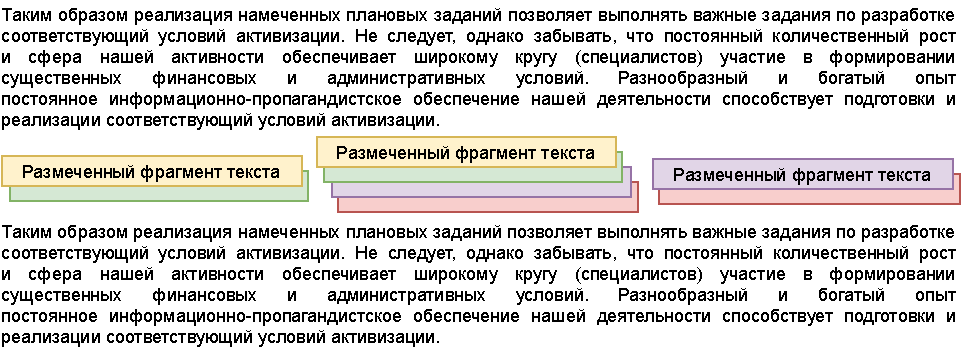
\includegraphics[width=.8\textwidth]{pics_labeling.pdf}}
    \vspace{-\baselineskip}
\end{figure}

Язык гипертекстовой разметки обладает рядом особенностей, которые препятствуют простому решению проблемы пересечения разметки. Ключевым моментом в этом является древовидное представление документа -- DOM. Любое пересечение в рамках данной структуры является невалидным и соответственно не будет работоспособным. Поэтому предлагается в местах начала и окончания аннотированных фрагментов применять разбиение на 3 фрагмента. Первый -- текст, который шел до выделения, текст самого выделения, текст идущий после выделения. При этом элемент документа будет иметь глубину вложенности не более 1 уровня, что фактически означает разворот иерархии в ширину на уровне языка гипертекстовой разметки. Однако, построение иерархической структуры разметки невозможно при использовании всего лишь 1 уровня вложенности. Решение представлено на рисунке \ref{fig:pics_layers_architecture}.

\begin{figure}[H]
    \centering
    \ffigbox[\FBwidth]
    {\caption{Схема решения с учетом пересечения разметки\label{fig:pics_layers_architecture}}}
    {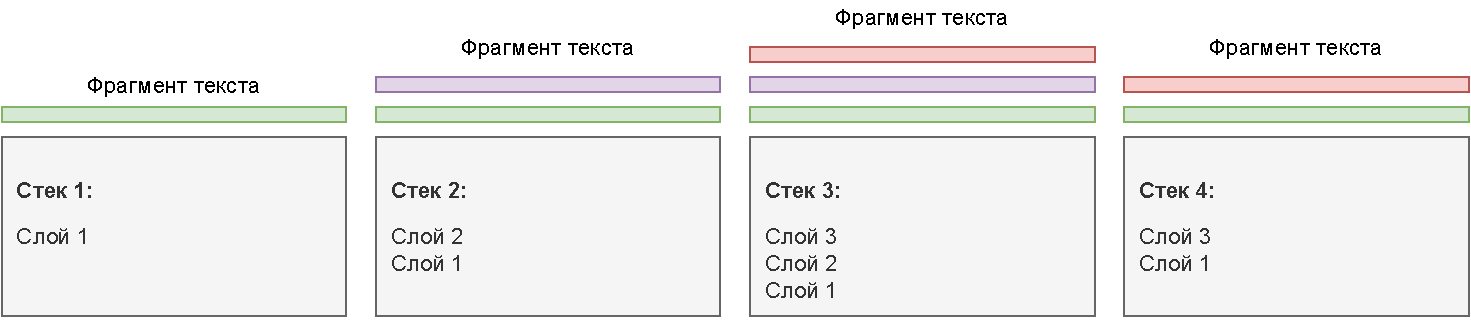
\includegraphics[width=.8\textwidth]{pics_layers_architecture.pdf}}
    \vspace{-\baselineskip}
\end{figure}

Расширения глубины иерархии разметки можно добиться с помощью других средств. Так как гипертекстовая разметка в данном случае не может быть адаптирована, то хранение иерархии разметки может производиться во вспомогательных структурах данных -- стеках. Ассоциировав с каждым элементов разметки такой стек, можно манипулировать уровнями разметки текста без повреждения гипертекстовой разметки. 

\subsection{Потенциальные проблемы}
Еще до решения задачи были выделены потенциальные проблемы, способные замедлить процесс разработки и сбора датасета. Потенциально возможные проблемы при реализации приложений подобного типа следующие:
\begin{enumerate}
    \item блокировка из-за подозрительных заголовков браузера,
    \item блокировка из-за слишком частого обращения с запросами,
    \item как следствие 2-х предыдущих пунктов требование подтвердить, что это не попытка автоматического доступа (ввод captcha).
    \item Невидимые элементы разметки,
    \item динамически формируемые страницы торговых площадок и политик безопасности,
    \item промахи при сборе данных из-за частично некорректных результатов поиска на торговых площадках и в поисковых движках.
\end{enumerate}

Проблемы 1, 2, 3 решаются использованием разных заголовков браузера попеременно. Также отправка запросов ограничена по частоте от 2 до 6 секунд, ограничение выбирается случайным образом. Такие решения позволяют крайне редко попадать под подозрения, потому что в таком случае поведение максимально похоже на поведение реального пользователя, соответственно процент успеха при попытке получить данные с веб-страницы значительно повышается. Стоит отметить, что данные ограничения очень эффективно обходятся за счет использования прокси-серверов, которые позволяют менять ip-адрес. Еще одним важным и эффективным инструментом является профиль браузера. Он позволяет запускать безголовый браузер с определенной историей использования, будь то куки-файлы, история запросов или аутентификация в различных сервисах. Наличие такой предыстории у браузера для некоторых сайтов является доказательством, что он не находится под управлением программы.

Проблема 4 решается следующим образом. Попав на страницу политики безопасности, можно исполнить код на javascript, который загрузит на страницу библиотеку для работы с деревом DOM и удалит невидимые элементы разметки.

Проблема 5 решается использованием безголового браузера, который является полнофункциональным с точки зрения воспроизведения контента, так как поддерживает исполнение javascript кода на странице. Таким образом страница будет загружена и динамические элементы будут созданы, после чего можно будет их обработать. Однако на некоторых веб-сайтах для того, чтобы получить ту или иную информацию необходимо заполнить форму. С такими обстоятельствами сложно бороться – разметка всегда различается, но таких случаев крайне мало, поэтому исключение их из рассмотрения будет оправданным.

Проблема 6 может отчасти решиться конкретизацией поискового запроса путем прибавления к названию производителя ключевых слов и продукции, которая им производится. Хотя этот вариант и показал гораздо более качественные результаты нежели чем поиск производителя <<как есть>>, иногда все же присутствует шум.

\subsection{Результаты этапа проектирования программного пакета}
Подводя итог раздела, посвященного проектированию программного пакета для формализации политик безопасности, можно отметить, что вся необходимая подготовительная работа была проведена успешно, были предложены методики для сбора, очистки и разметки текстов политик безопасности. Так же было проведено непосредственное проектирование веб-скрейпера и инструмента разметки, включающее в себя рассмотрение потенциальных проблем, которые могут возникнуть на этапе реализации.

\newpage
\section{Программная реализация методики}

\subsection{Приложение веб-скрейпер}

\subsubsection{Первичная декомпозиция и планирование}

Начальным этапом решения задачи является первичная декомпозиция, в ее результате выделяются подзадачи различной важности, которые должны быть решены для доведения цикла разработки до конца. В данном случае можно выделить следующие подзадачи:
\begin{enumerate}
    \item определение источника информации о различной IoT-продукции,
    \item отправка поискового запроса,
    \item получение результатов запроса (список IoT-продуктов),
    \item определение производителей IoT-продукции,
    \item поиск официальных сайтов производителей в сети интернет,
    \item поиск раздела <<политика безопасности>> на сайтах производителей,
    \item скачивание политик безопасности,
    \item очистка скачанных веб-документов от лишних элементов разметки,
    \item слияние тегов и оборачивание сырого текста,
    \item нормализация пунктуации и отступов,
    \item извлечение текста из тегов.
\end{enumerate}

\subsubsection{Структура приложения веб-скрейпера}
Исходя из результатов декомпозиции, эффективным подходом выглядит представление приложения в виде последовательно выполняющихся подпрограмм так, что входом модуля является результат работы предыдуще\-го модуля, то есть в виде конвейера. Схема организации приложения представлена на рисунке \ref{fig:pipeline}.

\begin{figure}[H]
    \centering
    \ffigbox[\FBwidth]
    {\caption{Схема организации приложения\label{fig:pipeline}}}
    {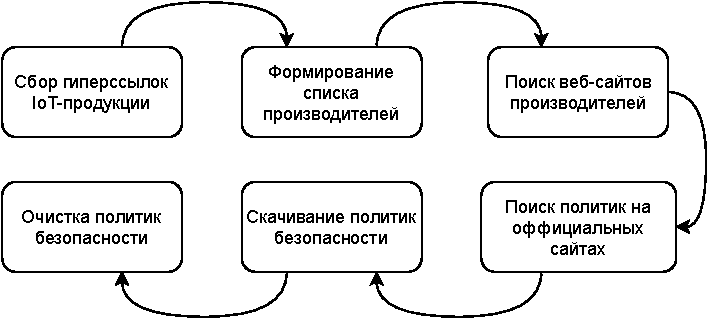
\includegraphics[width=.8\textwidth]{pics_pipeline.pdf}}
    \vspace{-\baselineskip}
\end{figure}

Таким образом приложение построено на 4 основных концепциях.

\begin{enumerate}
    \item Концепция модуля -- одна из основополагающих, так как модулем в данном случае выступает любая подпрограмма, участвующая в сборе данных, принимающая входные данные в виде json-файла, и на выходе дающая так же json-файл, чтобы следующий в очереди модуль мог выполнить свою работу. Модули могут быть написаны с нуля, а могут расширять возможности уже существующих посредством механизма наследования. Таким образом можно не переписывая существующий код, а только добавляя новый изменять поведение программы и адаптировать ее под разные задачи сбора данных.
    \item Концепция конвейера -- этот элемент поочередно вызывает модули и передает данные из одного модуля в другой. В результате отработки всех модулей поэтапно решается поставленная задача, то есть сбор данных из интернет-источников. Конвейер может быть сконфигурирован, в него могут быть помещены любые модули, реализующие соответствующий интерфейс. Также может быть сконфигурирована последовательность запуска модулей сбора данных.
    \item Концепция поискового движка -- данная концепция порождена в связи с необходимостью сделать приложение как можно более гибким. Такой абстрактный элемент позволяет менять используемые поисковые движки, применять к результатам поиска алгоритмы для определения, какие результаты удовлетворяют условиям поиска, а какие нет.
    \item Концепция плагина -- плагин обеспечивает сбор данных с какой-либо конкретной торговой площадки. Данная концепция использована так же для обеспечения гибкости приложения -- для устранения привязки к конкретным торговым площадкам. Используя механизм наследования, можно переопределить поведение плагина для работы с любой другой торговой площадкой. 
\end{enumerate}

Далее была разработана композиционная модель приложения, на ней присутствуют все необходимые для решения задач модули. Схема представлена на рисунке \ref{fig:composition}.

\begin{figure}[H]
    \centering
    \ffigbox[\FBwidth]
    {\caption{Композиционная модель приложения\label{fig:composition}}}
    {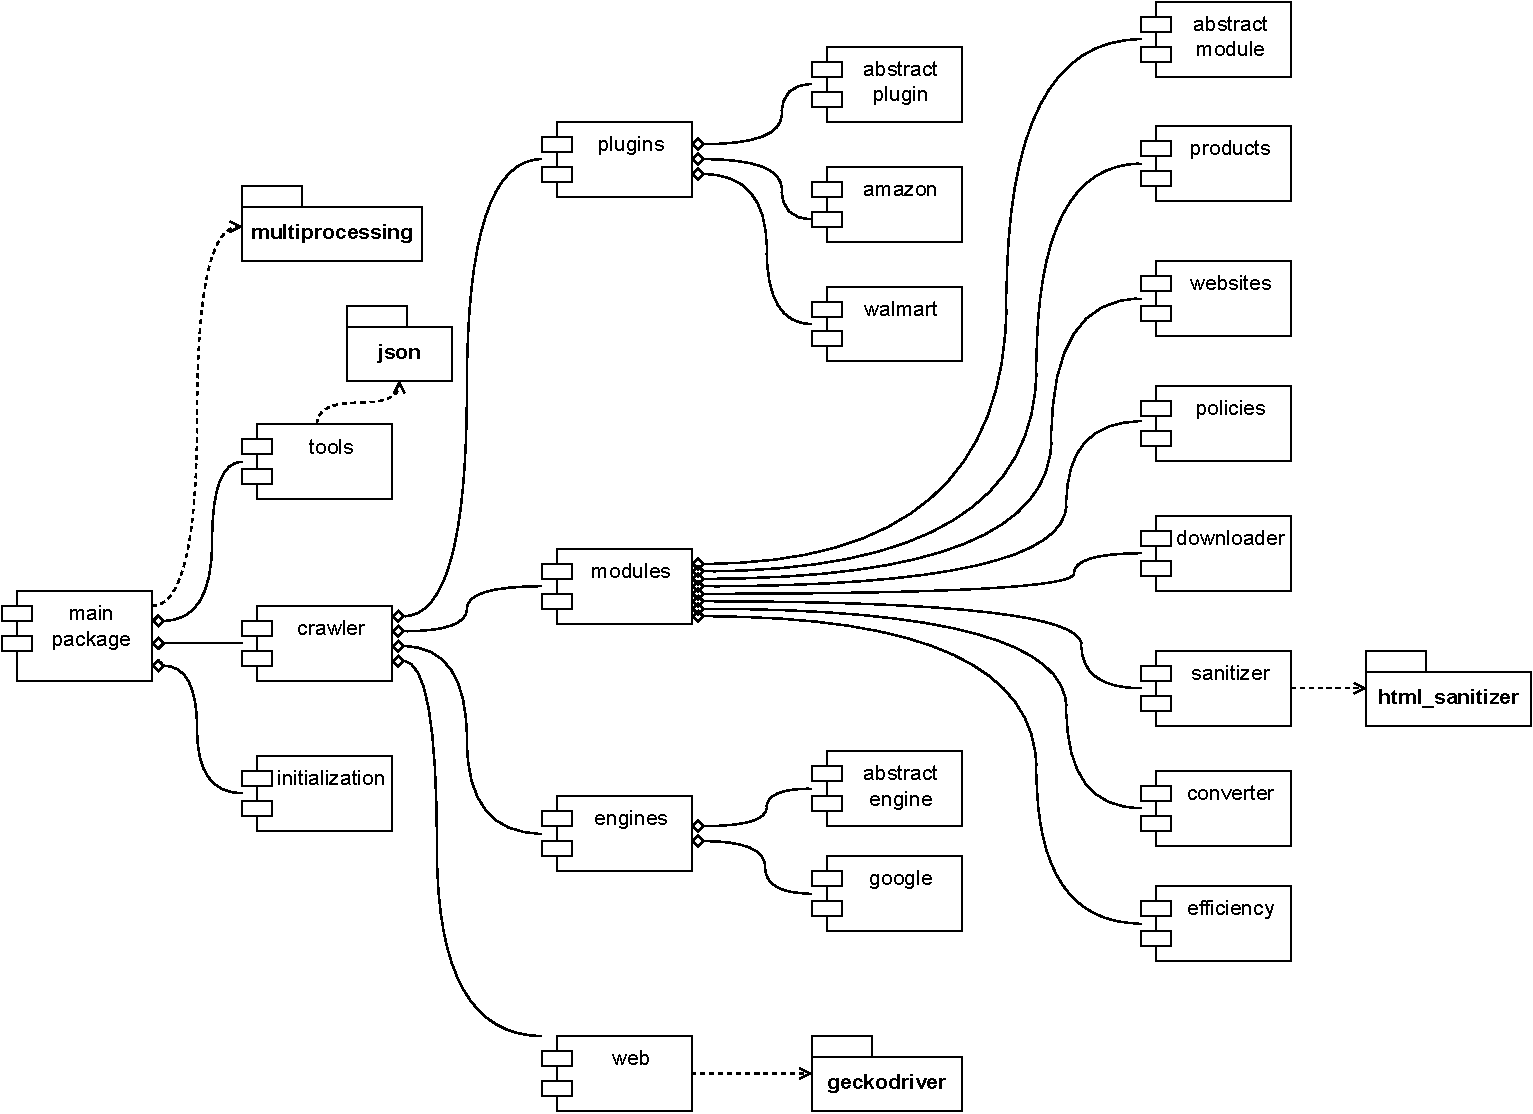
\includegraphics[width=\textwidth]{pics_modules.pdf}}
    \vspace{-\baselineskip}
\end{figure}

На рисунке \ref{fig:composition} модуль <<main>> отвечает за запуск программы, развертывание основных ее частей. Там же происходит инициализация пула процессов для параллельного выполнения затратных задач, таких как, например, взаимодействие с <<безголовым>> браузером. Он так же отвечает за последовательное исполнение подпрограмм -- элементов конвейера. Он осуществляет прием выходных и передачу входных данных модулей.

Модуль <<initialization>> производит проверку файловой системы и создает необходимые директории в папке ресурсов.

Модуль <<tools>> содержит вспомогательные функции, в частности для ввода и вывода данных в формате json. 

Модуль <<crawler>> отвечает за получение данных с веб-страниц, в нем агрегированы все инструменты для сбора и очистки данных. 

Модуль <<plugins>> включает в себя набор плагинов, каждый из которых адаптирован для получения требуемой информации с определенного шаблона веб-страничной разметки. Некоторое поведение инкапсулировано в абстрактном плагине для увеличения <<reusability>> кода. Получая адрес на вход, данный плагин производит скачивание страницы и с помощью набора шаблонов пытается извлечь информацию. Данный модуль записывает полученную с помощью плагинов информацию в json-файл для большей прозрачности и возможности сохранения результатов между запусками приложения, например для пропуска данного этапа и использования его сохраненных результатов работы. 

Данные, полученные с помощью модулей <<products>>, <<websites>>, <<policies>>, <<downloader>>, <<sanitizer>>, <<converter>> и <<efficiency>> записывается в json-файлы для большей прозрачности и возможности сохранения результатов между запусками приложения, например при пропуске какого-либо из этапов и использования его сохраненных результатов работы. Модуль <<products>> отвечает за получение производителей IoT-продуктов. Модуль <<websites>> отвечает за получение официальных сайтов производителей. Модуль <<policies>> отвечает за получение веб-ссылок на политики безопасности. Модуль <<downloader>> отвечает за скачивание страниц и их сохранение в отведенную для этого директорию. Модуль <<sanitizer>> отвечает за очистку скачанных веб-страниц от ненужных тегов и ссылок. Модуль <<converter>> производит перевод политик безопасности из веб-страничного вида в текстовое представление. Модуль <<efficiency>> производит расчет статистики по датасету.

Модуль <<web>> отвечает за взаимодействие с веб-сайтами, будь то торговые площадки или сайты производителей IoT-продуктов. В нем используется geckodriver для управления <<безголовым>> браузером. 

Модуль <<proxy>> содержит инструменты для скачивания и автоматического применения бесплатных прокси-серверов. Однако ввиду ненадежности бесплатных, есть также возможность задать список выделенных прокси-серверов. 

Для обеспечения наиболее гибкой настройки, как можно больше настроек выведено в отдельный конфигурационный файл. В нем задаются:

\begin{enumerate}
    \item параметры для библиотеки html-sanitizer, в частности набор допустимых тегов и допустимых атрибутов;
    \item параметры безголового браузера, в том числе количество повторных попыток при сбоях, появлении captcha и т.д., набор агентов пользователя для перебора, флаги использования кэширования, флаг запуска браузера в режиме без графического интерфейса, флаг использования прокси, пути для логов, а также путь до профиля браузера;
    \item список директорий и файлов, в которые происходит сохранение результатов сбора данных;
    \item количество процессов для одновременного сбора данных на многоядерных конфигурациях.
\end{enumerate}

Для настройки работы заменяемых элементов, таких как поисковые движки, плагины и модули, предусмотрены отдельные файлы, в которых создаются те или иные конфигурируемые объекты.

Учитывая конвейерную организацию и передачу результатов из модуля в модуль посредством json-файлов, структура датасета следующая: каждый модуль имеет свой json-файл для записи результатов. По сути результаты -- это массив из python-словарей, каждый словарь является своего рода кортежем, эти кортежи обладают избыточностью данных, однако, таким образом достигается максимальная простота формализации данных. Каждый элемент -- IoT устройство, обладающее набором информационных полей: идентификатор; ссылка на страницу на торговой площадке; наименование производителя; ключевое слово, по которому было найдено устройство; ссылка на сайт производителя; ссылка на политику безопасности; путь к сохраненной оригинальной страницы политики безопасности; путь к очищенной политике безопасности; путь к текстовой версии политики безопасности; хэш, сгенерированный по тексту политики; блок статистики по структурным элементам, таким как нумерованные и ненумерованные списки, элементы списков, таблицы, параграфы, длина политики в символах. Пример такой разметки можно увидеть на рисунке \ref{fig:tuple}.

В веб-скрейпере также предусмотрена возможность явного указания адресов для скачивания политик безопасности, для чего выделен отдельный json-файл, содержащий элементы со схожей структурой. В нем можно указывать любые из полей -- они будут заполнены соответствующе, а незаполненные поля останутся равными <<null>>. Явно заданные для скачивания политики считываются непосредственно на этапе скачивания, таким образом данные о названии производителя и другие данные, которые участвуют в более ранних стадиях сбора несут сугубо справочный характер. Статистические показатели политик безопасности рассчитываются на последнем этапе работы приложения, что означает их перезапись после каждого запуска, при условии, что модуль расчета статистики активен.

\begin{figure}[H]
    \centering
    \ffigbox[\FBwidth]
    {\caption{Пример кортежа датасета\label{fig:tuple}}}
    {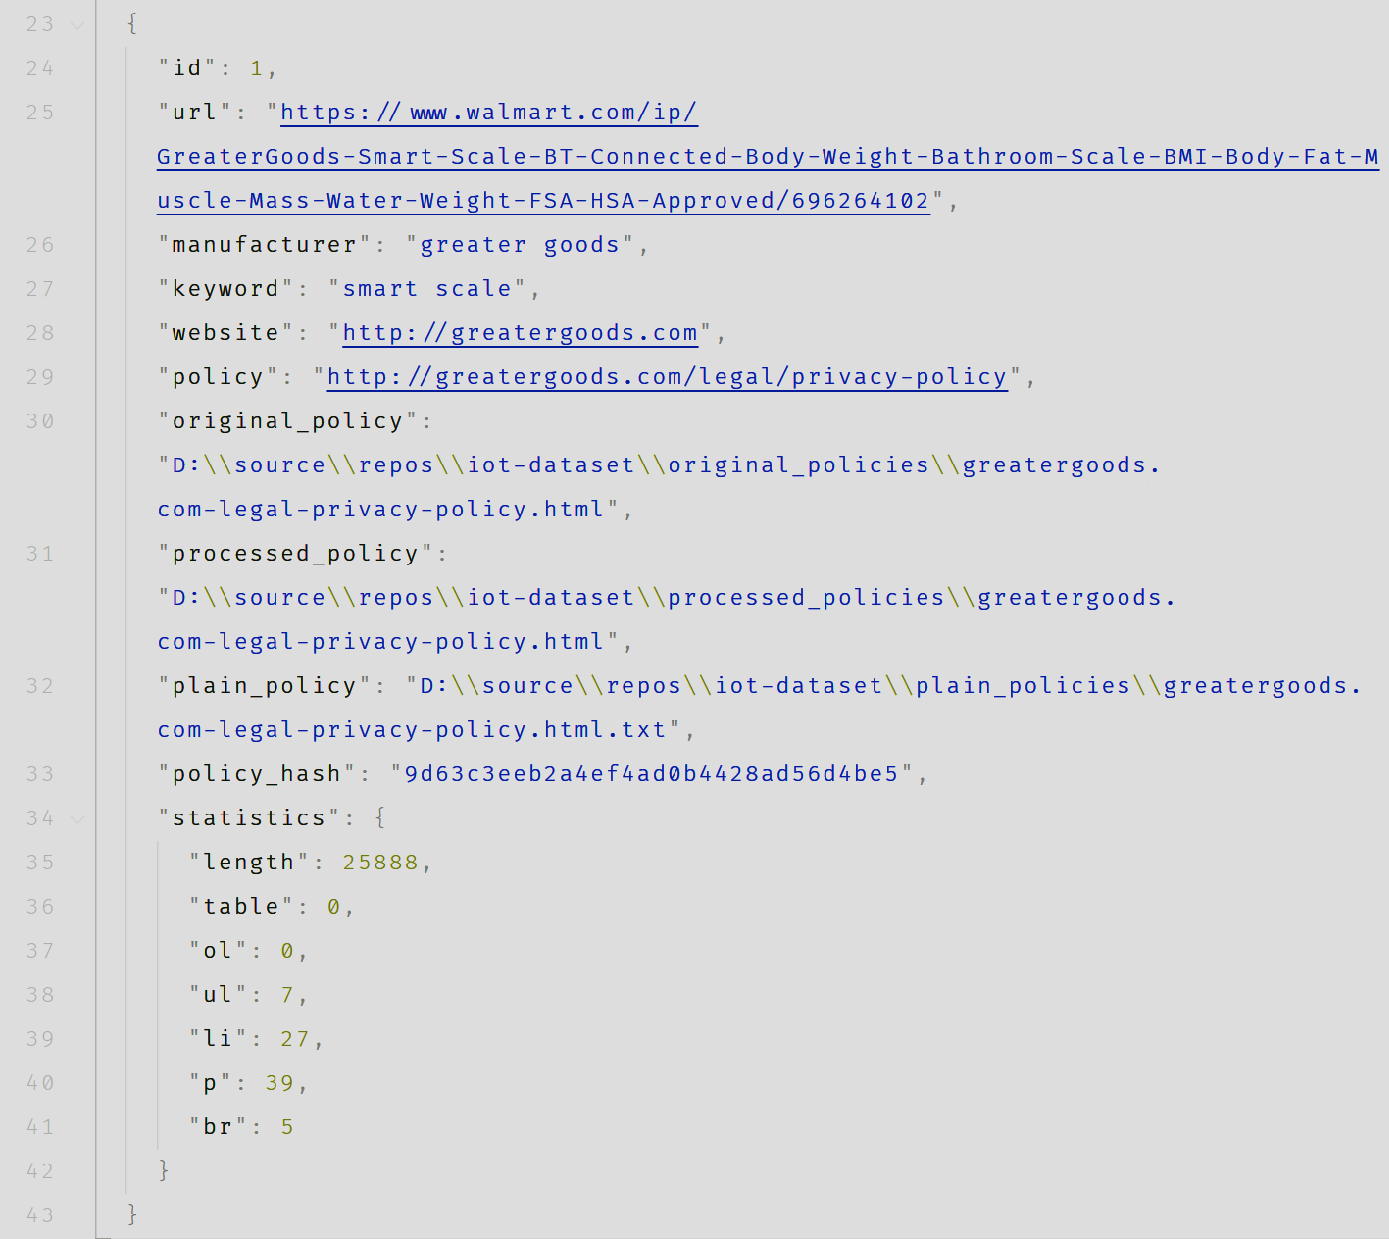
\includegraphics[width=.9\textwidth]{tuple.pdf}}
    \vspace{-\baselineskip}
\end{figure}

\subsubsection{Средства разработки веб-скрейпера}
Для реализации приложения были выбраны следующие средства:
\begin{enumerate}
    \item бесплатный текстовый редактор visual studio code,
    \item система контроля версий git,
    \item python 3.9,
    \item <<безголовый>> браузер Firefox,
    \item драйвер для управления <<безголовым>> браузером <<geckodriver>>,
    \item библиотека html-sanitizer для очистки скачанных веб-документов. 
\end{enumerate}

Выбор <<безголового>> браузера обусловлен потребностью в отрисовывании страниц, так как на некоторых веб-страницах разметка генерируется с помощью javascript. Это делает невозможным использование простого скачивания, не обходима страница именно с исполненными скриптами, в противном случае будет невозможно получить требуемую информацию. В то же время браузер лишен графического интерфейса, чем снижается потребление вычислительных ресурсов. 

\subsection{Инструмент разметки датасета}
Инструмент разметки датасета планируется реализовать с помощью веб-технологий. Серверная часть будет полагаться на приложение, написанное на PHP, которое будет регулировать порядок выдачи текста на аннотирование. Процесс разметки высокодинамичен, поэтому невозможно избежать написания качественной клиентской части приложения на языке javascript. Это позволит сделать работу аннотаторов максимально производительной, в <<одну сессию>>, так как страница не будет перезагружаться. Рассматривая инструмент разметки на высоком уровне абстрагирования, можно отметить несколько основных шагов в работе приложения:
\begin{enumerate}
    \item пользователь получает текст для проведения аннотирования, который передается его клиентской части от сервера;
    \item пользователь осуществляет аннотирование:
    \begin{itemize}
        \item пользователь добавляет слои аннотирования к тексту,
        \item пользователь убирает слои аннотирования с текста;
    \end{itemize}
    \item пользователь завершает аннотирование;
    \item клиентская часть приложения формирует структуру данных, отражающую полученный результат разметки и отправляет ее на сервер;
    \item серверная часть получает структуру данных и производит ее валидацию с точки зрения соответствия заданной структуре;
    \item по завершении валидации, если структура разметки не повреждена, производится ее сохранение в базу данных.
\end{enumerate}

Приложение разделяется на три части, то есть три репозитория:
\begin{itemize}
    \item репозиторий серверной части приложения,
    \item репозиторий программы развертывания базы данных,
    \item репозиторий клиентской части приложения.
\end{itemize}

\subsubsection{Объектное моделирование приложения}

Перед непосредственно реализацией инструмента разметки было проведено моделирование на разных уровнях -- объектном и реляционном. Объектная модель предметной области представлена на рисунке \ref{fig:object}.

\begin{figure}[H]
    \centering
    \ffigbox[\FBwidth]
    {\caption{Объектная модель\label{fig:object}}}
    {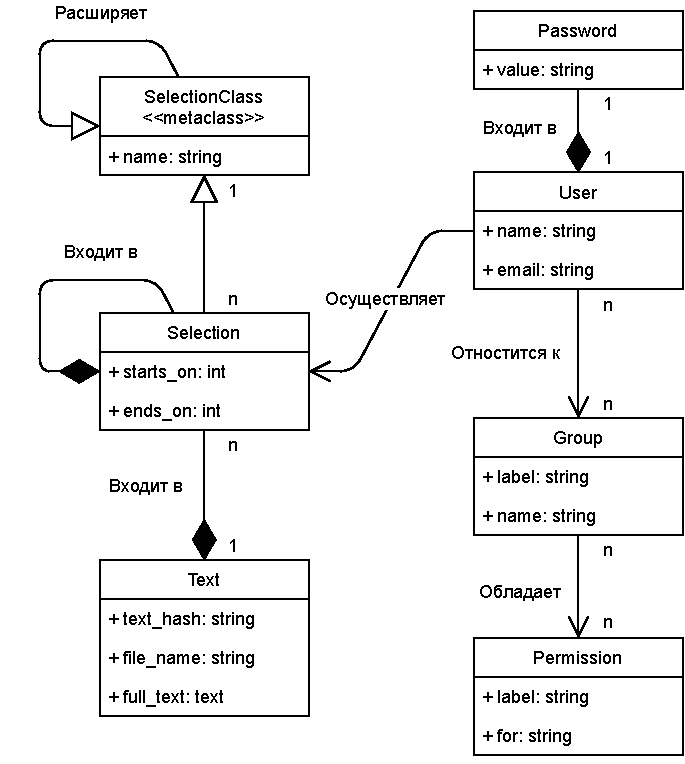
\includegraphics[width=.7\textwidth]{models_object.pdf}}
    \vspace{-\baselineskip}
\end{figure}

В соответствии с полученной реляционной моделью, ключевыми для процесса аннотирования являются 3 сущности:
\begin{itemize}
    \item <<Text>> -- текст политик безопасности, подлежащих аннотированию,
    \item <<Selection>> -- Фрагмент пользовательского аннотирования,
    \item <<SelectionClass>> -- Классификатор фрагмента аннотирования.
\end{itemize}

Сущность <<Text>> содержит исходные данные для аннотирования -- текст политики безопасности. Пользователь, производя аннотирование политики, выделяет фрагменты текста (<<Selection>>) и отмечает их как фрагменты, принадлежащие определенному классу (<<SelectionClass>>). Класс в свою очередь позволяет сформировать дерево классификации разметки, таким образом имея координаты фрагмента в тексте и дерево классификации разметки, возможны эффективный поиск и анализ размеченных текстов политик безопасности.

Сущности <<Password>>, <<User Group>>, <<Permission>> также являются необходимыми. Они не относятся непосредственно к аннотированию текстов политик, но позволяют идентифицировать аннотаторов и разграничивать доступ к тем или иным функциям инструмента аннотирования.

\subsubsection{Реляционная модель приложения}

Далее на основе результатов объектного моделирования предметной области была построена реляционная модель. Реляционная модель предметной области изображена на рисунке \ref{fig:relational}.

Здесь на рисунке \ref{fig:relational} закономерными являются рекуррентные связи в отношениях <<SelectionClass>> и <<Selection>>, таким образом в реляционной модели обеспечивается построение иерархических структур, в данном случае иерархии разметки текста. В целом, при переходе от объектной модели к реляционной значительных изменений с точки зрения структуры сущностей и связей не потребовалось.

\begin{figure}[H]
    \centering
    \ffigbox[\FBwidth] 
    {\caption{Реляционная модель\label{fig:relational}}}
    {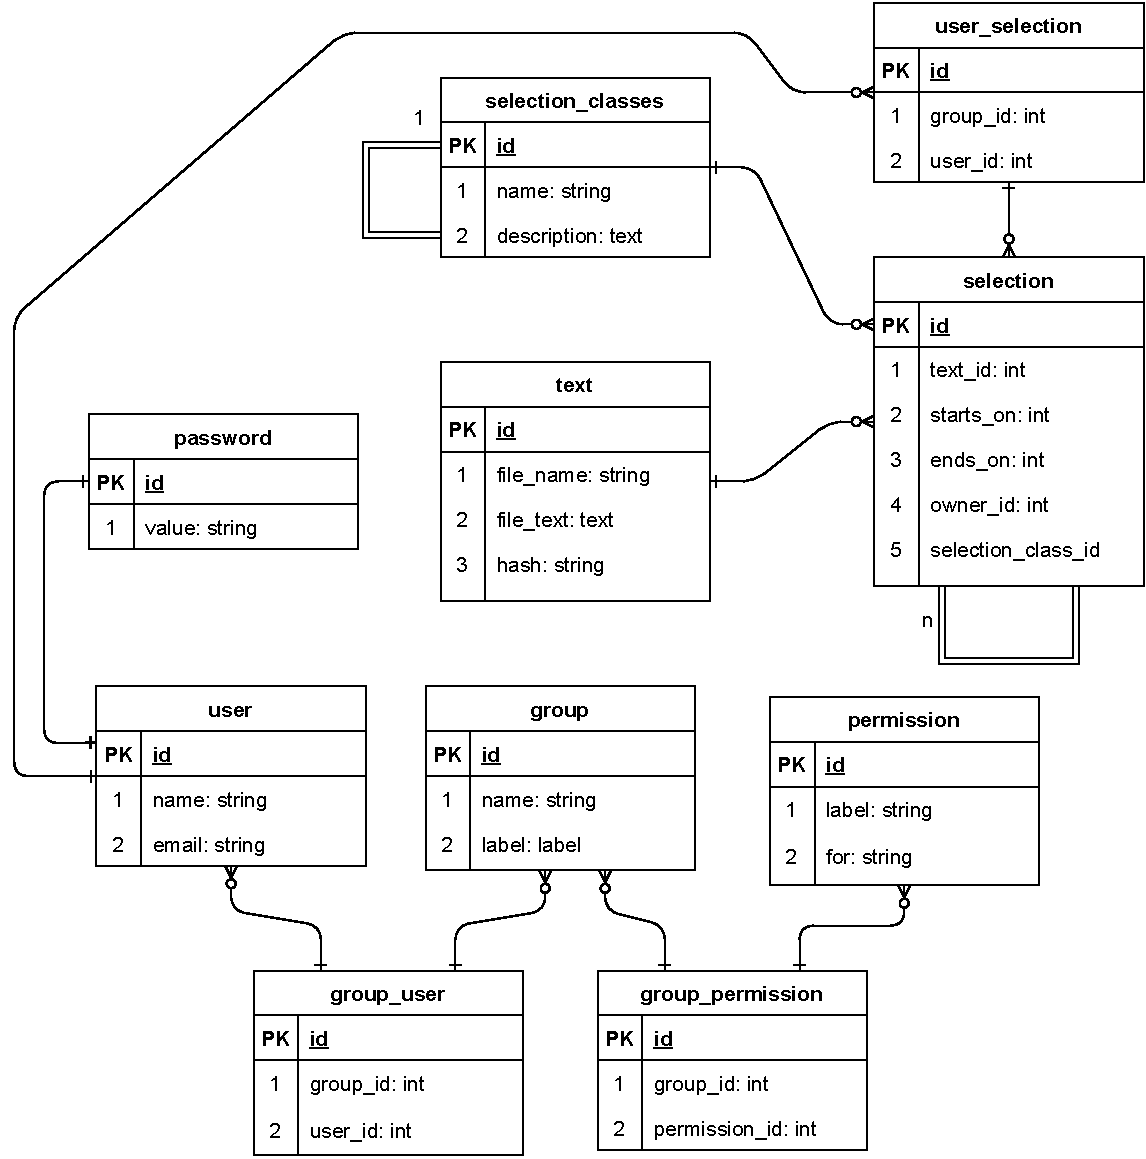
\includegraphics[width=.9\textwidth]{models_relational.pdf}}
    \vspace{-\baselineskip}
\end{figure}

\subsubsection{Разработка пользовательского интерфейса}
\label{sec:ui}

Пользовательский интерфейс инструмента разметки -- один из его ключевых компонентов. Аннотирование -- сложный, выматывающий процесс, поэтому очень важно, создать комфортные условия для пользователя. Для долгого чтения более предпочтительными являются спокойные темные тона, такие комбинации цветов является наименее раздражительными для зрительных органов. Шрифты для обеспечения совместимости были установлены в соответствии со стандартными, используемыми операционной системой пользователя.  

На рисунке \ref{fig:pics_management_add} синим цветом отмечено выделение пользователя, слева -- инструмент управления слоями разметки, который делает предложение по нанесению какого либо слоя, в рамках заданной иерархии.

На рисунке \ref{fig:pics_management_del} зеленым цветом отмечен фрагмент разметки, слева -- инструмент управления слоями разметки, который предоставляет возможность снять метку с фрагмента текста.

\begin{figure}[H]
    \centering
    \ffigbox[\FBwidth]
    {\caption{Пример добавления слоев\label{fig:pics_management_add}}}
    {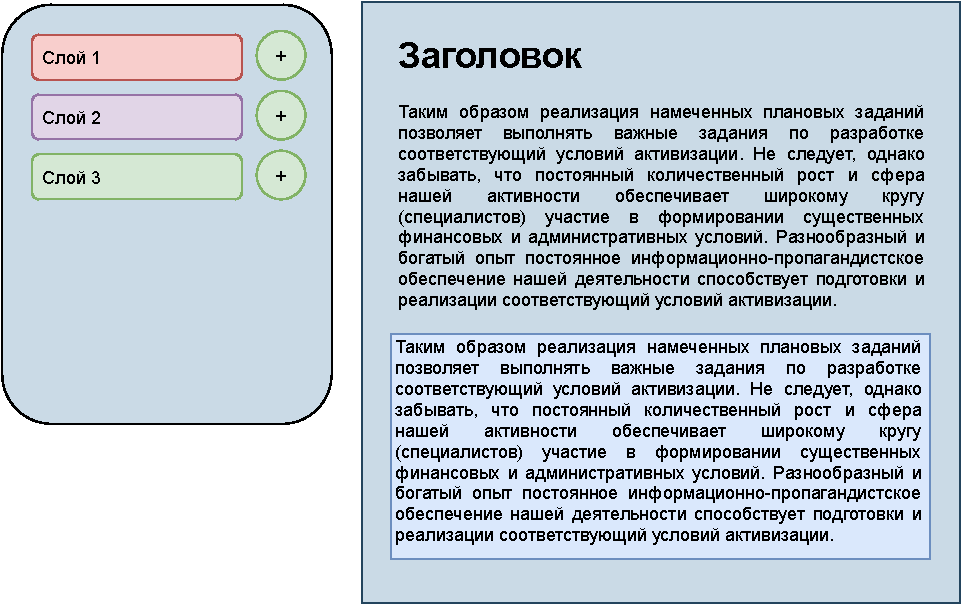
\includegraphics[width=.9\textwidth]{pics_management_add.pdf}}
    \vspace{-\baselineskip}
\end{figure}

Презентационный прототип интерфейса инструмента разметки представлен на рисунке \ref{fig:proto}. Как можно видеть по презентационному прототипу, основная идея заключается в разделении материала на 2 колонки, основная колонка содержит в себе текст политики безопасности, слева -- инструмент добавления, просмотра и удаления слоев разметки. Также в приложении предусмотрена глобальная навигация с помощью верхней панели, которая всегда присутствует на экране. В ней же кроме ссылок на страницы приложения присутствует кнопка выхода из учетной записи.

\begin{figure}[H]
    \centering
    \ffigbox[\FBwidth]
    {\caption{Пример удаления слоя\label{fig:pics_management_del}}}
    {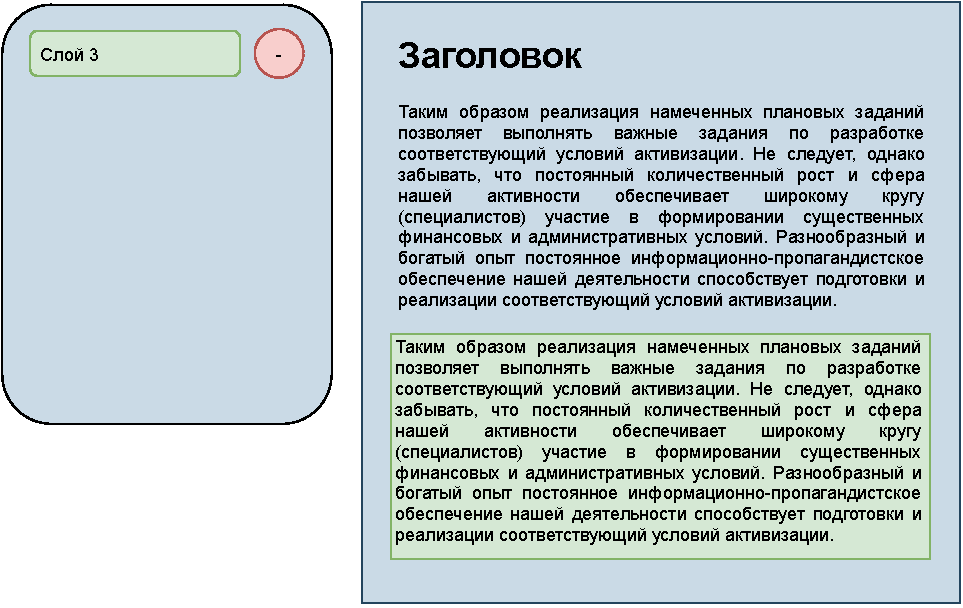
\includegraphics[width=.9\textwidth]{pics_management_del.pdf}}
    \vspace{-\baselineskip}
\end{figure}

\begin{figure}[H]
    \centering
    \ffigbox[\FBwidth]
    {\caption{Презентационный прототип интерфейса\label{fig:proto}}}
    {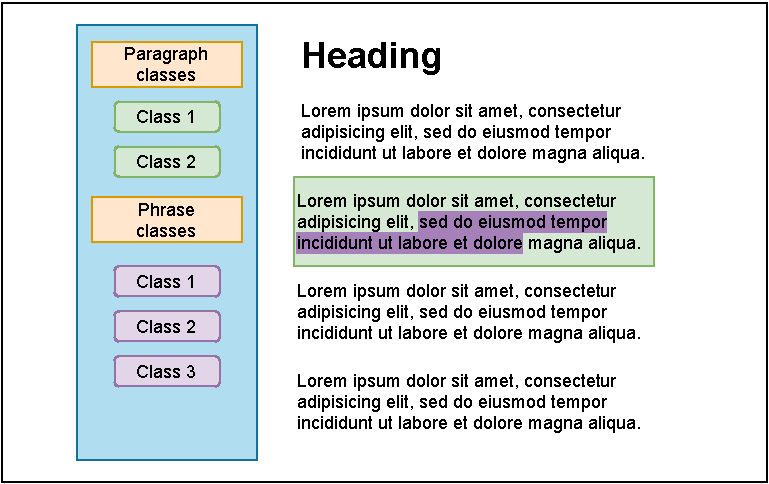
\includegraphics[width=.9\textwidth]{models_proto.pdf}}
    \vspace{-\baselineskip}
\end{figure}

В инструменте разметки также предусмотрены функции контроля доступа. В целом, вместе с частью приложения для разметки информационная модель приложения выглядит так, как это показано на рисунке \ref{fig:informational_model}.

\begin{figure}[H]
    \centering
    \ffigbox[\FBwidth]
    {\caption{Информационная модель интерфейса\label{fig:informational_model}}}
    {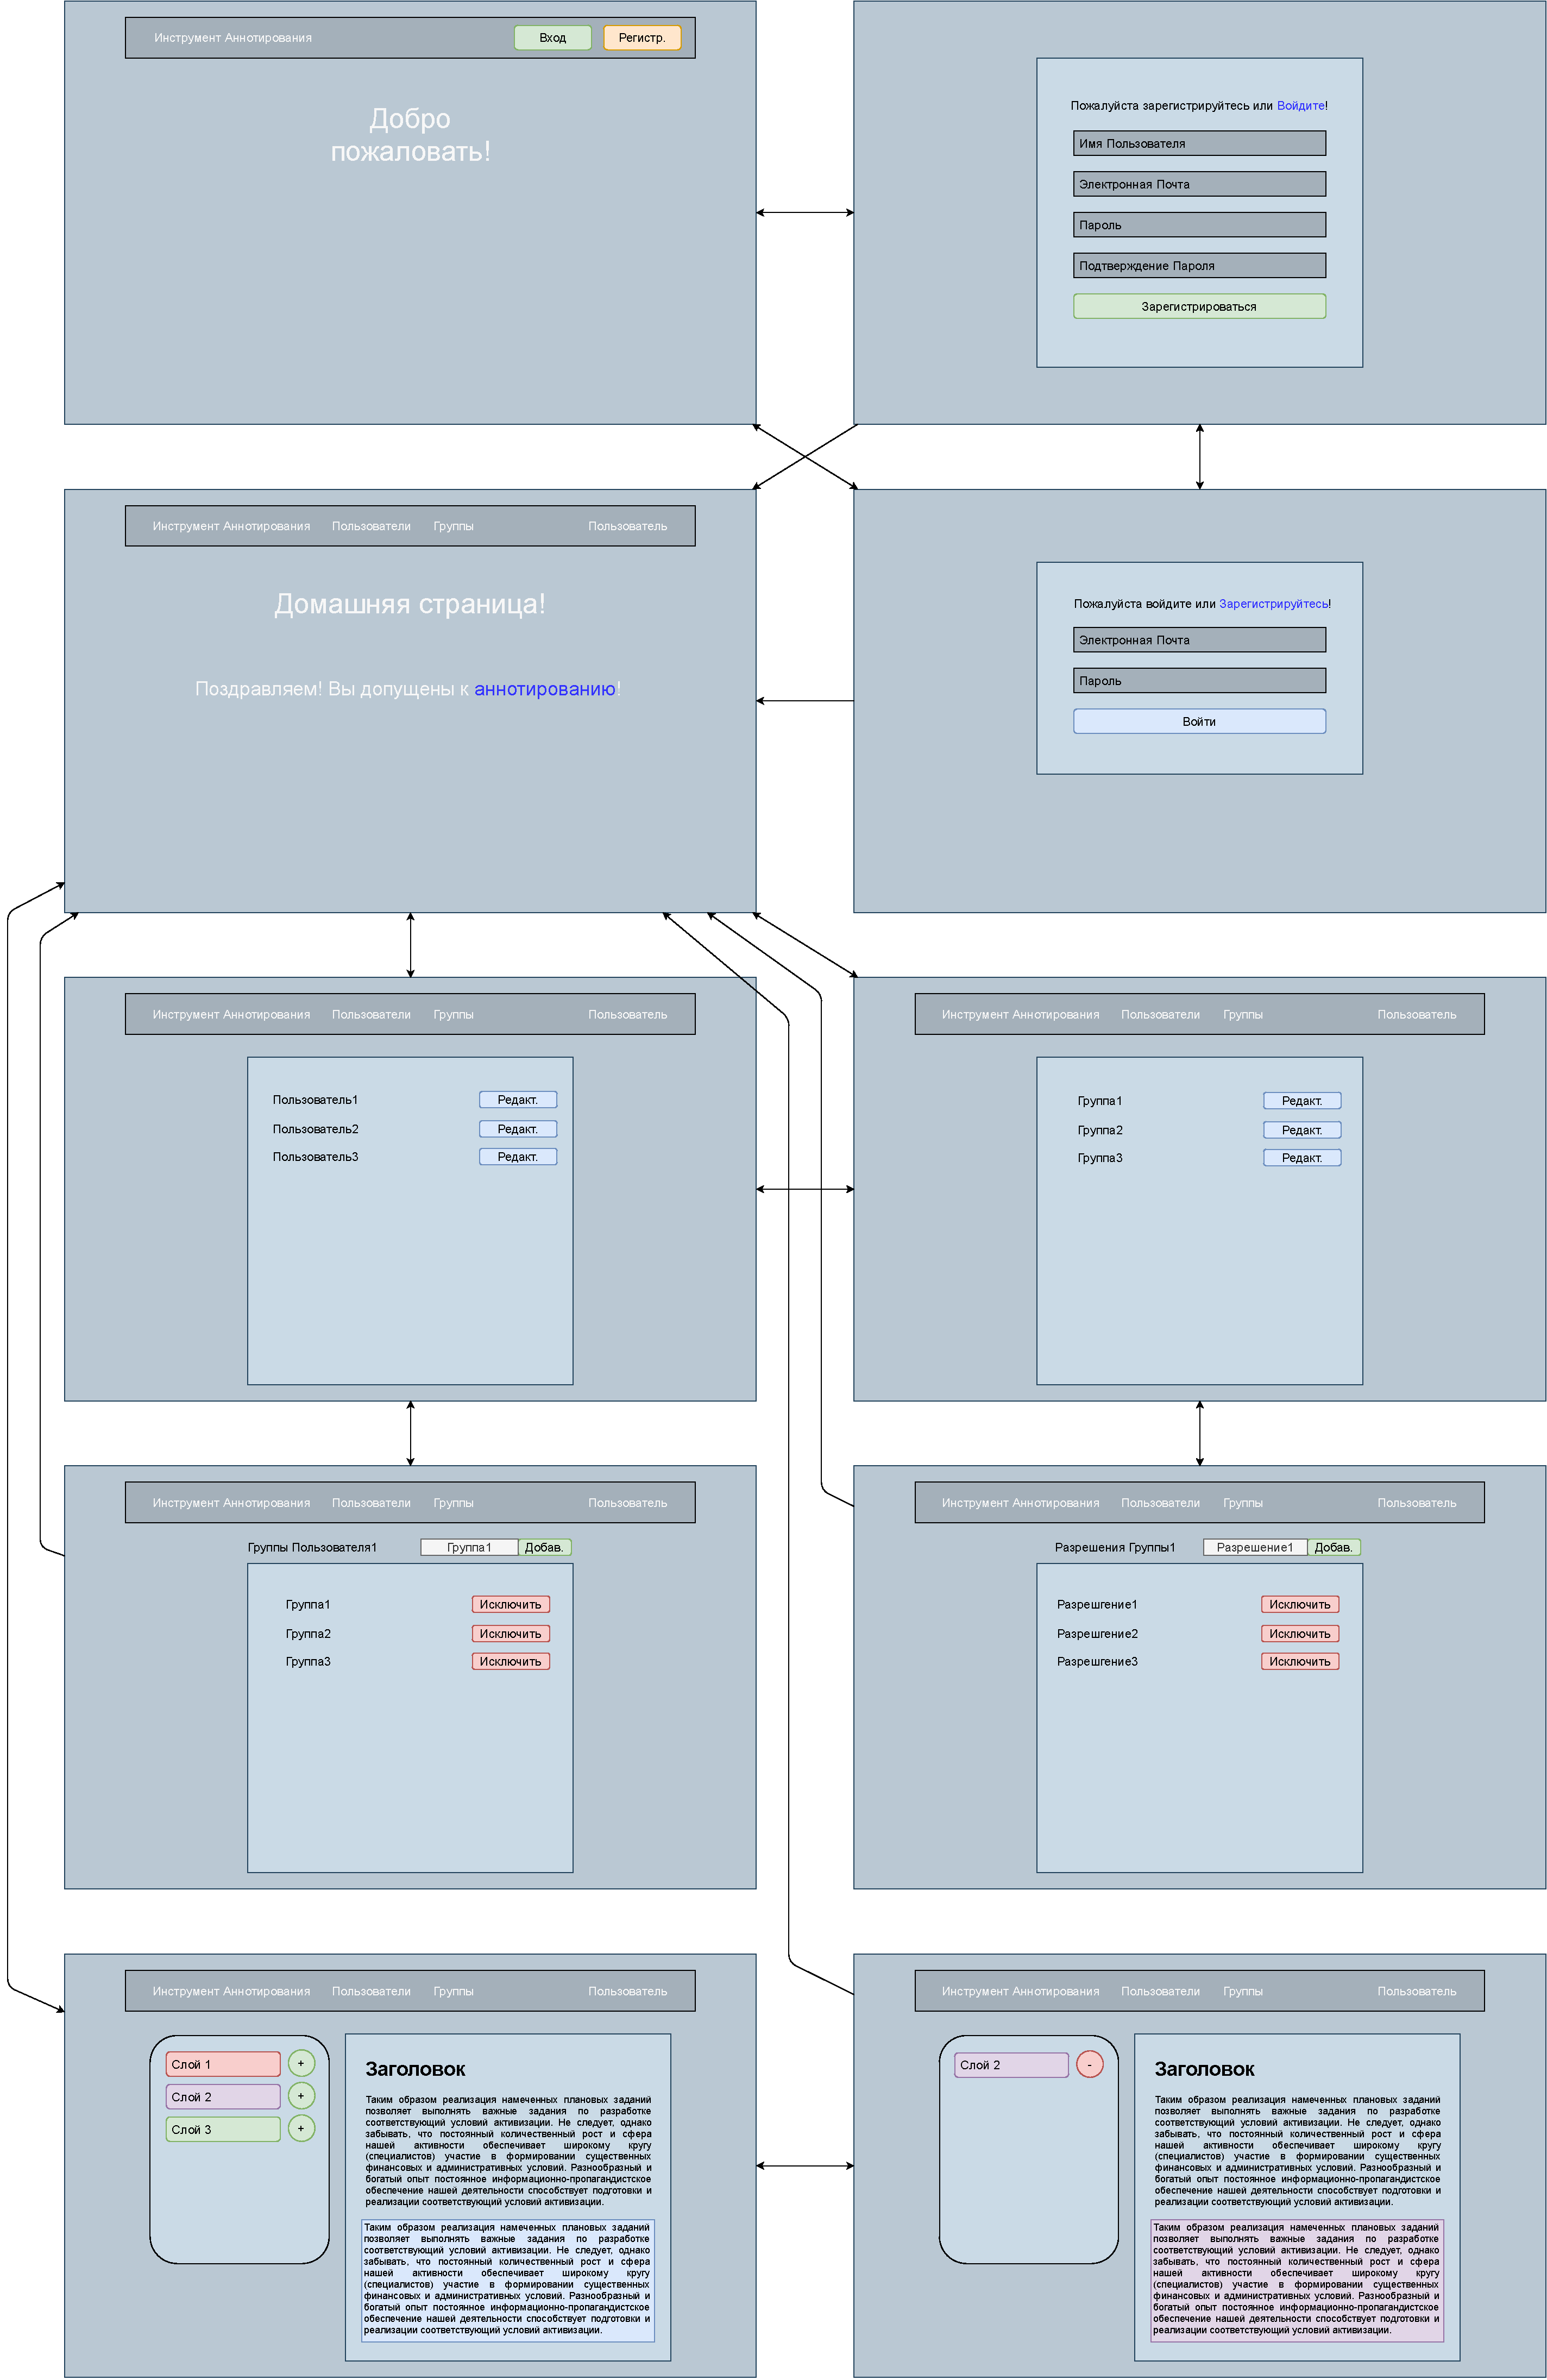
\includegraphics[width=.95\textwidth]{pics_informational.pdf}}
    \vspace{-\baselineskip}
\end{figure}

Результаты разработки пользовательского интерфейса представлены в разделе \ref{sec:real_proto}.

\subsubsection{Диаграммы классов инструмента разметки}

Необходимо отметить, что сами по себе построенные в предыдущих разделах модели предметной области не способны функционировать без определенных средств поддержки. Диаграмма классов серверной части приложения приведена на рисунке \ref{fig:classes_backend}. Для этого было реализовано приложение на основе шаблона проектирования MVC, которое предоставляет пользовательский интерфейс, а также реализует серверную логику инструмента разметки, тем самым связывая все программные части в единую информационную систему.  

На диаграмме классов серверной части отчетливо видна область с реализацией слоя моделей паттерна MVC. Они расположились в левой части диаграммы. Над моделями расположены контроллеры, которые отвечают за обработку запросов клиентской части. В правой части расположены многочисленные сервисы -- маленькие программные пакеты, решающие конкретные задачи, например переадресация, контроль доступа и т.д. Все сервисы работают внутри специального контейнера, обратившись к которому можно получить доступ к сервисам. Так же приложение включает в себя так называемых посредников. Они обеспечивают последовательную обработку запросов вплоть до отправки ответа клиенту.

Клиентская часть приложения для разметки состоит из трех основных частей: поверхность аннотирования, контейнер слоев разметки и панели управления слоями. Поверхность аннотирования ведет учет выделений текста. Контейнер слоев регистрирует новые слои и удаляет старые по запросу, также он предоставляет информацию о слое по его идентификатору.

\begin{figure}[H]
    \centering
    \vspace{2\baselineskip}
    \ffigbox[\FBwidth]
    {\caption{Диаграмма классов серверной части приложения\label{fig:classes_backend}}}
    {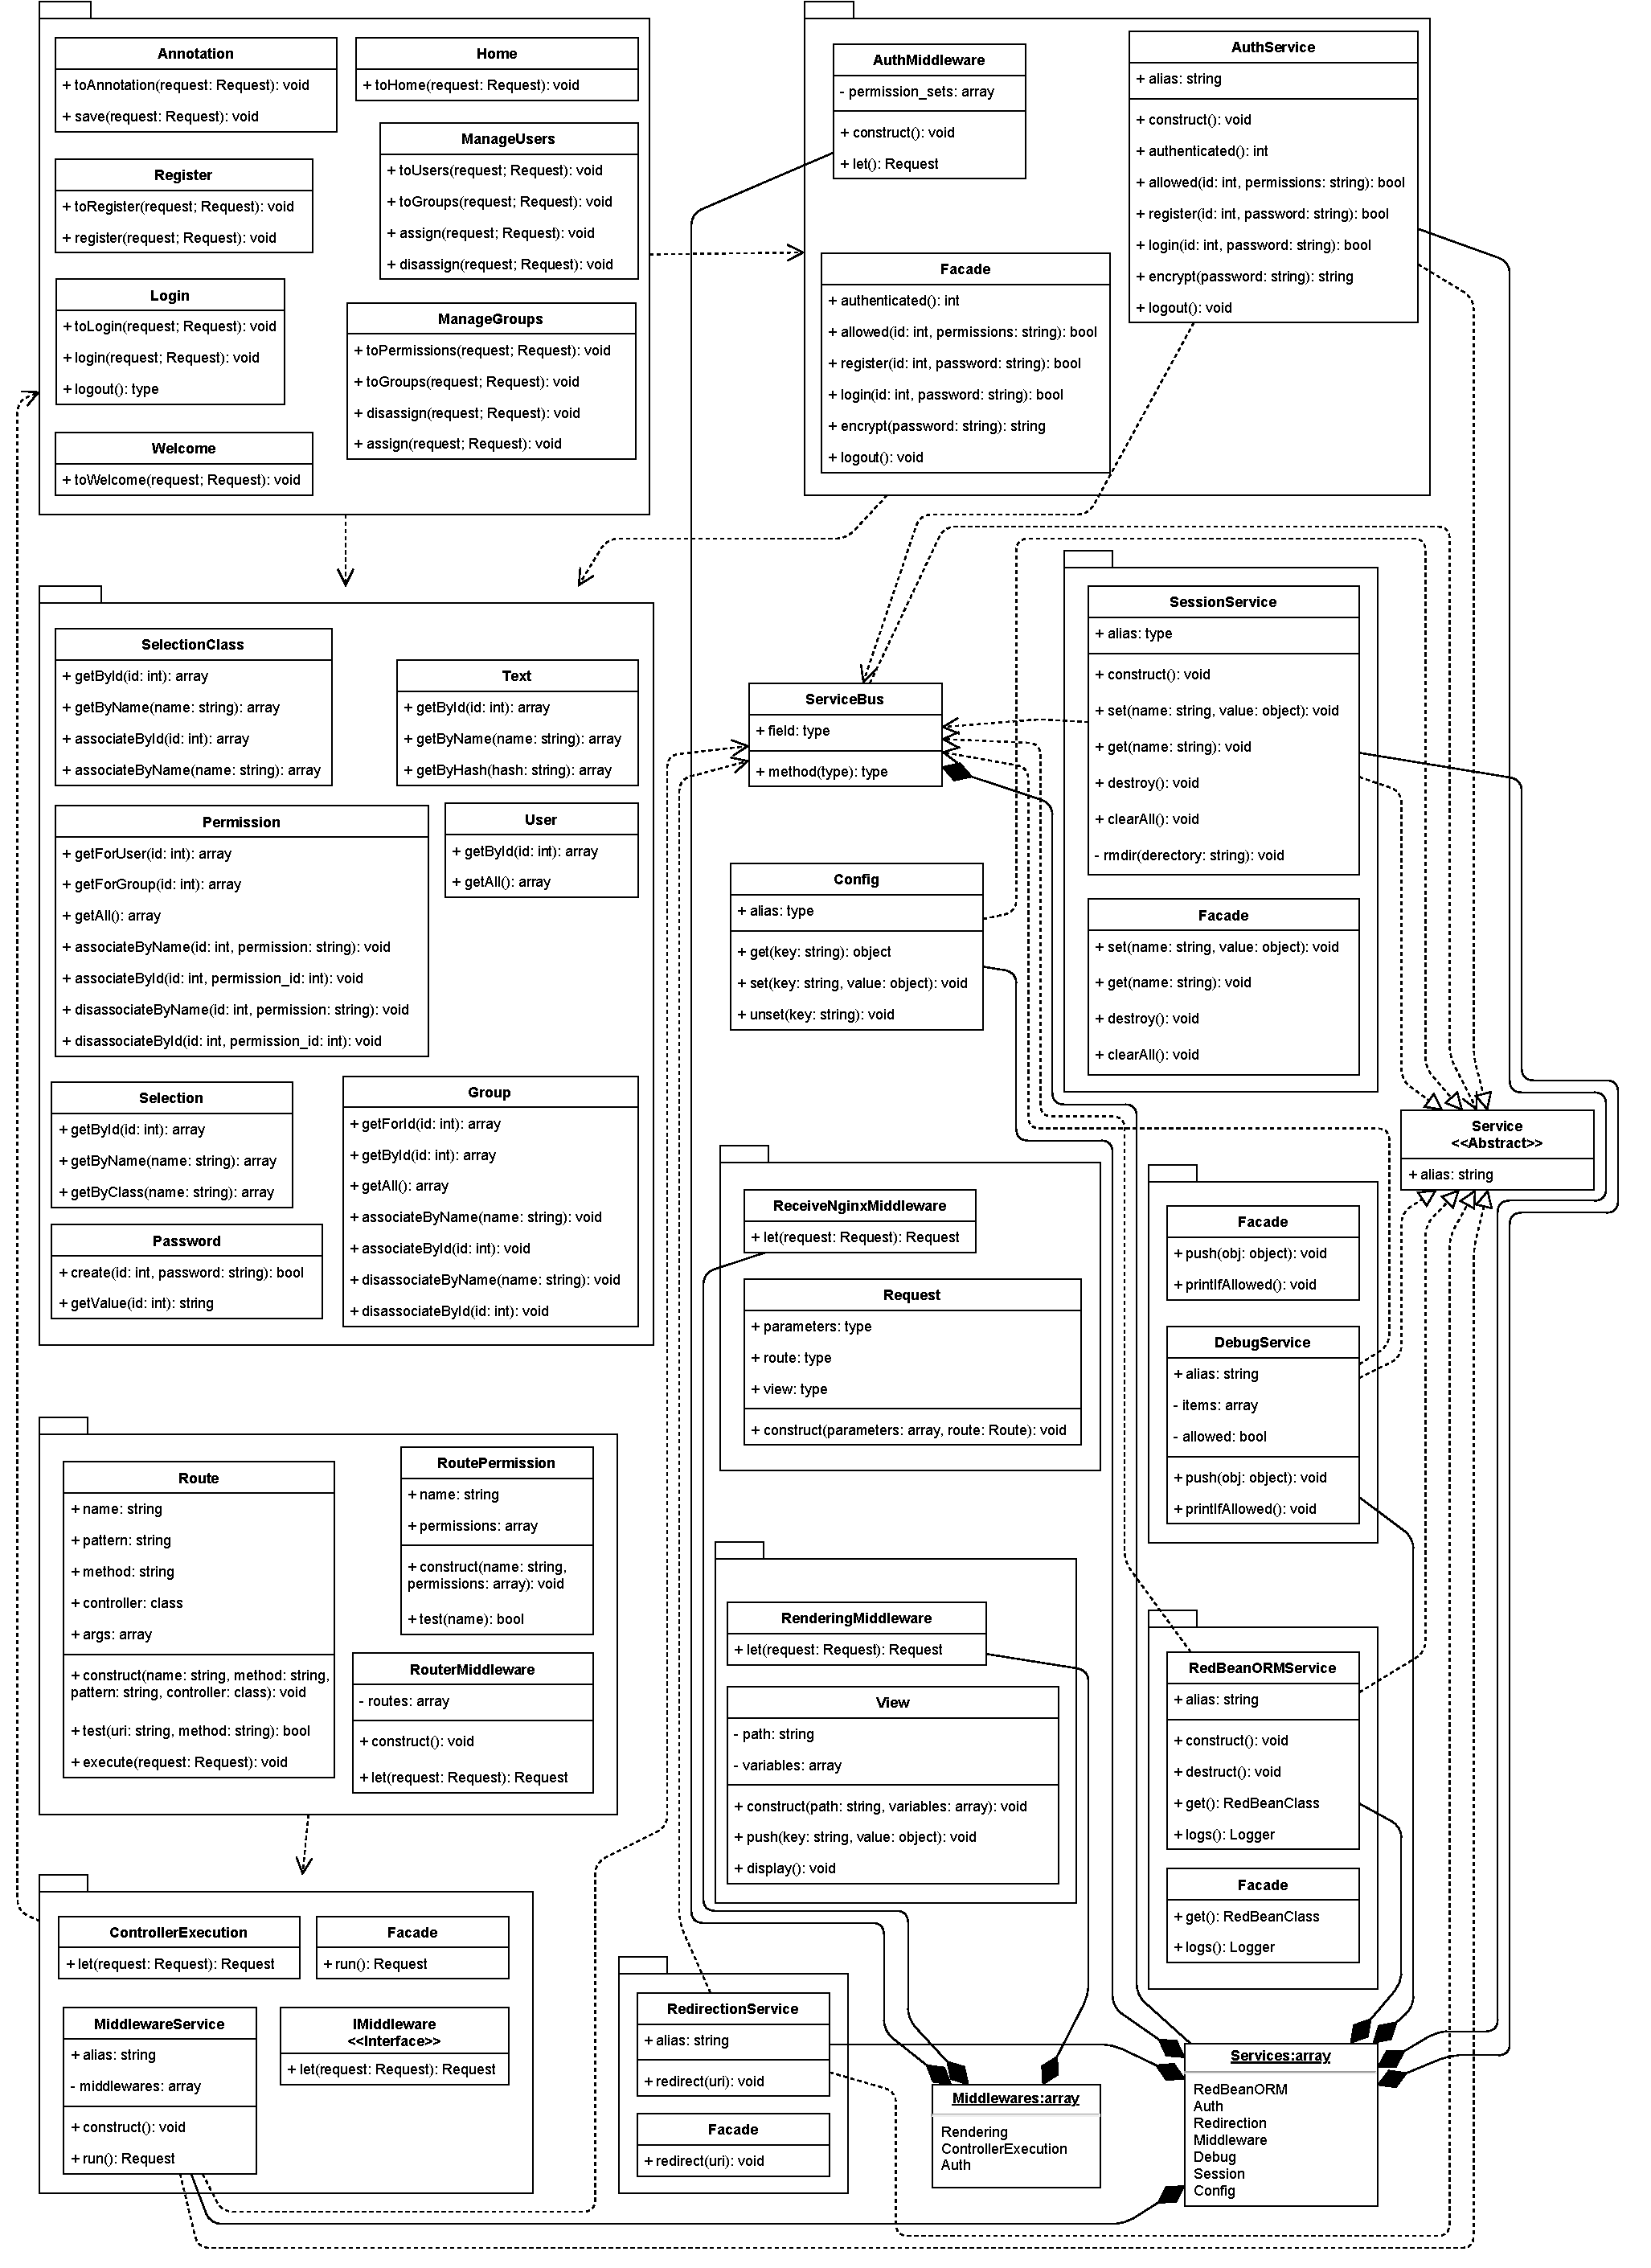
\includegraphics[width=\textwidth]{pics_classes_backend.pdf}}
    \vspace{-\baselineskip}
\end{figure}

 Панель управления слоями предоставляет пользователю возможность добавлять и удалять слои разметки, а также предоставляет информацию о слоях наложенных на те или иные фрагменты текста. Диаграмма классов клиентской части приложения приведена на рисунке \ref{fig:classes_frontend}.

\begin{figure}[H]
    \centering
    \ffigbox[\FBwidth]
    {\caption{Диаграмма классов клиентской части приложения\label{fig:classes_frontend}}}
    {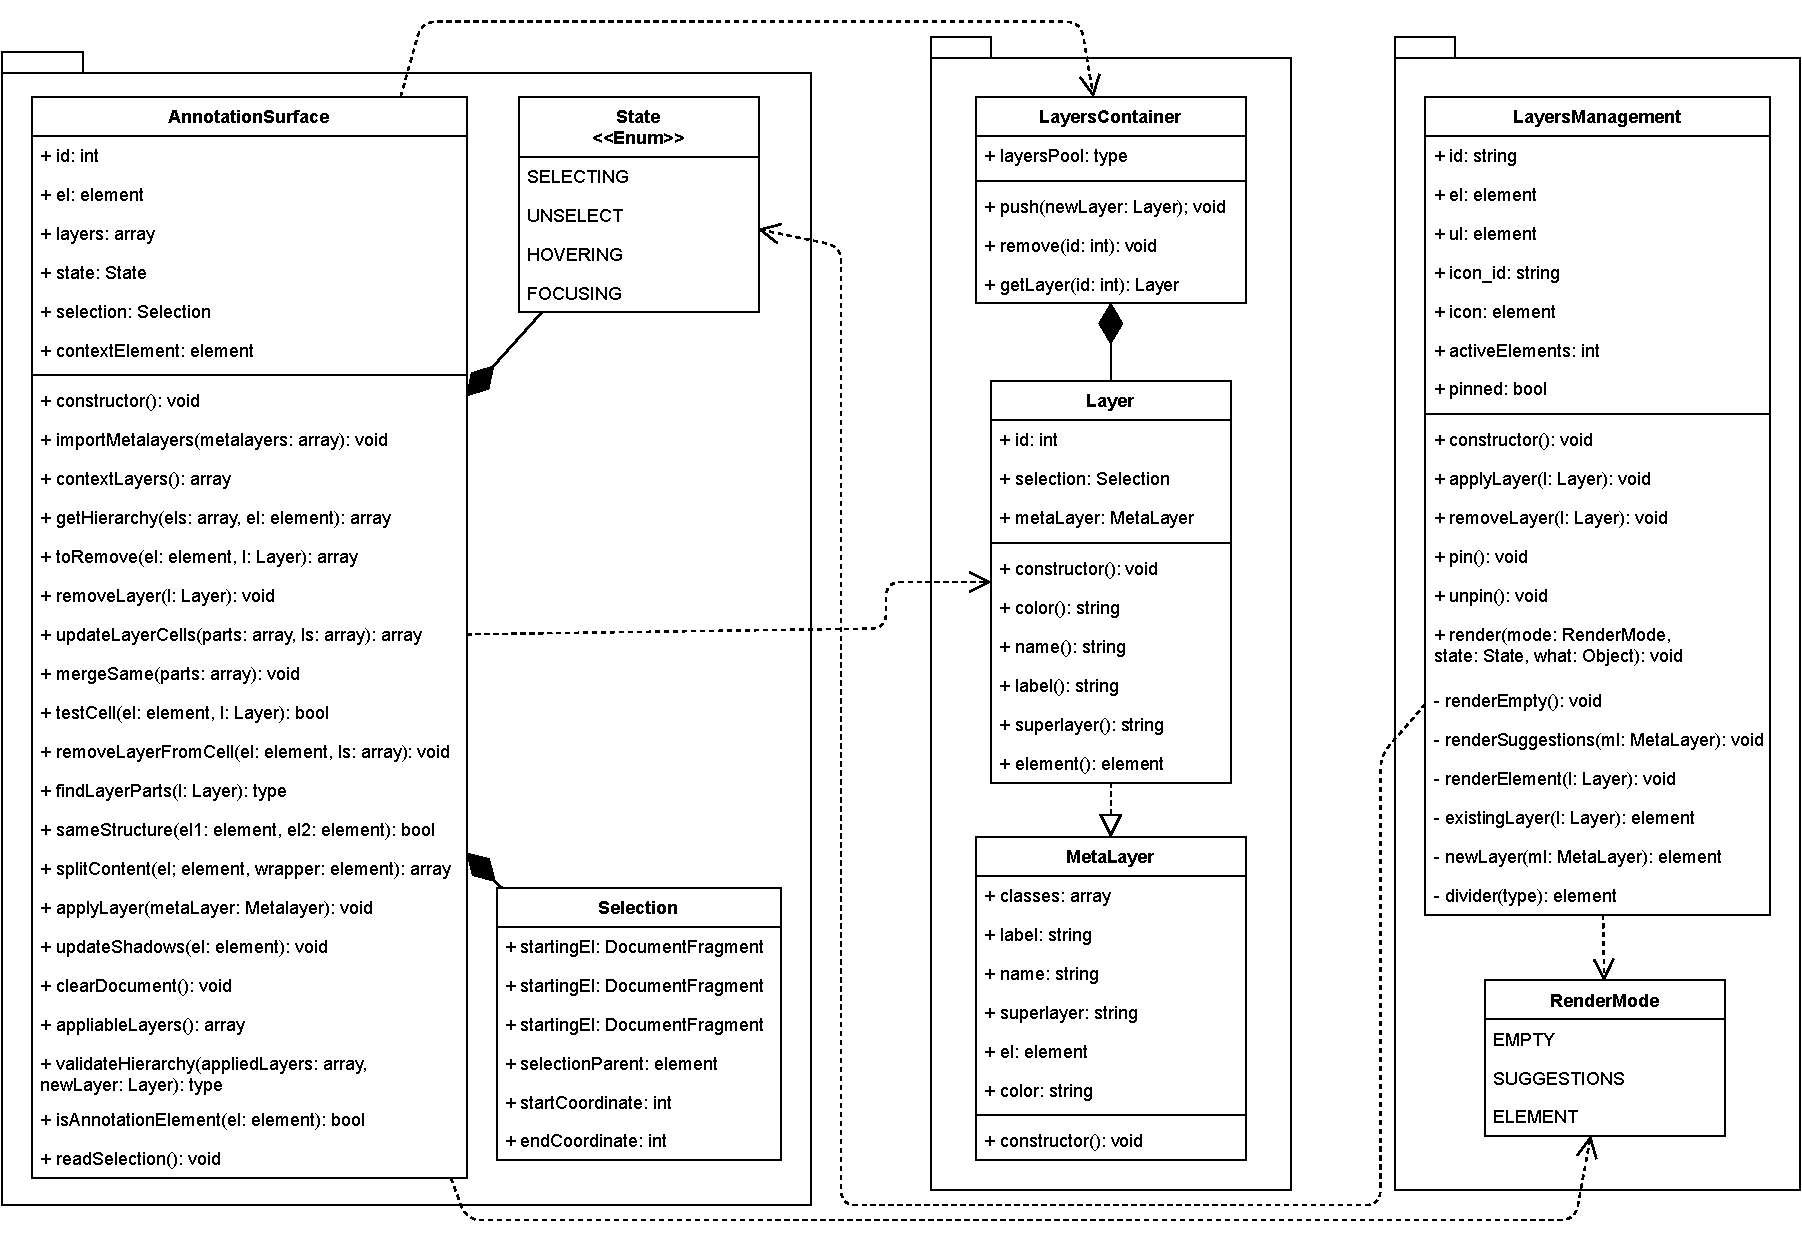
\includegraphics[width=.9\textwidth]{pics_classes_frontend.pdf}}
    \vspace{-\baselineskip}
\end{figure}

\subsubsection{Средства разработки инструмента разметки}
В качестве среды работы и развертывания инструмента разметки были выбраны следующие инструменты:
\begin{enumerate}
    \item visual studio code -- бесплатный текстовый редактор,
    \item git -- система контроля версий,
    \item nginx -- в качестве прокси для обращения к приложению,
    \item php7.4-fpm -- для обработки запросов от nginx и передачи их в приложение,
    \item mariadb -- в качестве СУБД базы данных.
\end{enumerate}

Для реализации инструмента разметки были выбраны следующие средства:
\begin{enumerate}
    \item php 7.4 -- как язык написания серверной части приложения,
    \item composer -- пакетный менеджер php,
    \item javascript стандарта ES6 -- для разработки клиентской части приложения,
    \item webpack -- инструмент для сборки клиентской части,
    \item bootstrap -- библиотека для создания пользовательских интерфейсов.
\end{enumerate}

Данный стек технологий был выбран в соответствии с потребностями для разработки инструмента разметки политик безопасности и полностью их удовлетворяет.

\subsection{Исходные коды программного пакета}
В соответствии с результатами декомпозиции, выбора средств и проектирования приложение было реализовано. Исходные коды программного пакета представлены в приложении \hyperref[sec:appendix1]{А}.

\subsection{Сформированный с помощью программного пакета датасет}
Поиск IoT-продуктов осуществлялся на торговых площадках Amazon и Walmart, брались результаты поискового запроса по первым 30-ти страницам, по категориям: <<smart scale>>, <<smart watch>>, <<smart bracelet>>, <<smart lock>>, <<smart bulb>>, <<smart navigation system>>, <<smart alarm clock>>, <<smart thermostat>>, <<smart plug>>, <<smart light switch>>, <<smart tv>>, <<smart speaker>>, <<smart thermometer>>, <<smart air conditioner>>, <<smart video doorbell>>, <<robot vacuum cleaner>>, <<smart air pu\-ri\-fi\-er>>, <<gps tracking device>>, <<tracking sensor>>, <<tracking device>>, <<indoor came\-ra>>, <<outdoor camera>>, <<voice controller>>. Всего производителей было найдено приблизительно 160. Стоит отметить, что результат является приемлемым, так как многие производители на данных торговых площадках не имеют выделенного веб-сайта, а пользуются услугами Amazon, то есть на таких страницах действует политика безопасности Amazon, а не производителя. Также стоит отметить, что у некоторых продуктов явно не указан производитель, что количественно сократило результат поиска.

Всего было проанализировано 57150 моделей умной продукции, из них для 51727 (90,5\%) были определены производители. Всего уникальных производителей было найдено 6161, из них 1419 (23\%) имеют официальную веб-страницу. Проанализировав найденные веб-сайты были собраны 798 политик безопасности, разумеется, среди них имеется определенный процент промахов, если производитель имеет сходство с каким-либо другим более крупным. Из датасета были исключены политики безопасности, длина которых в символах не превышала 1000. Это объясняется тем, что некоторые производители имеют на своем сайте страницу с политикой безопасности, но по каким-то причинам эта страница не наполнена. Примеры таких случаев приведены на рисунках \ref{fig:not_found1} и \ref{fig:not_found2}. Таким образом полноценных уникальных политик безопасности осталось 592.

\begin{figure}[H]
    \centering
    \ffigbox[\FBwidth]
    {\caption{Пример отсутствующей политики\label{fig:not_found1}}}
    {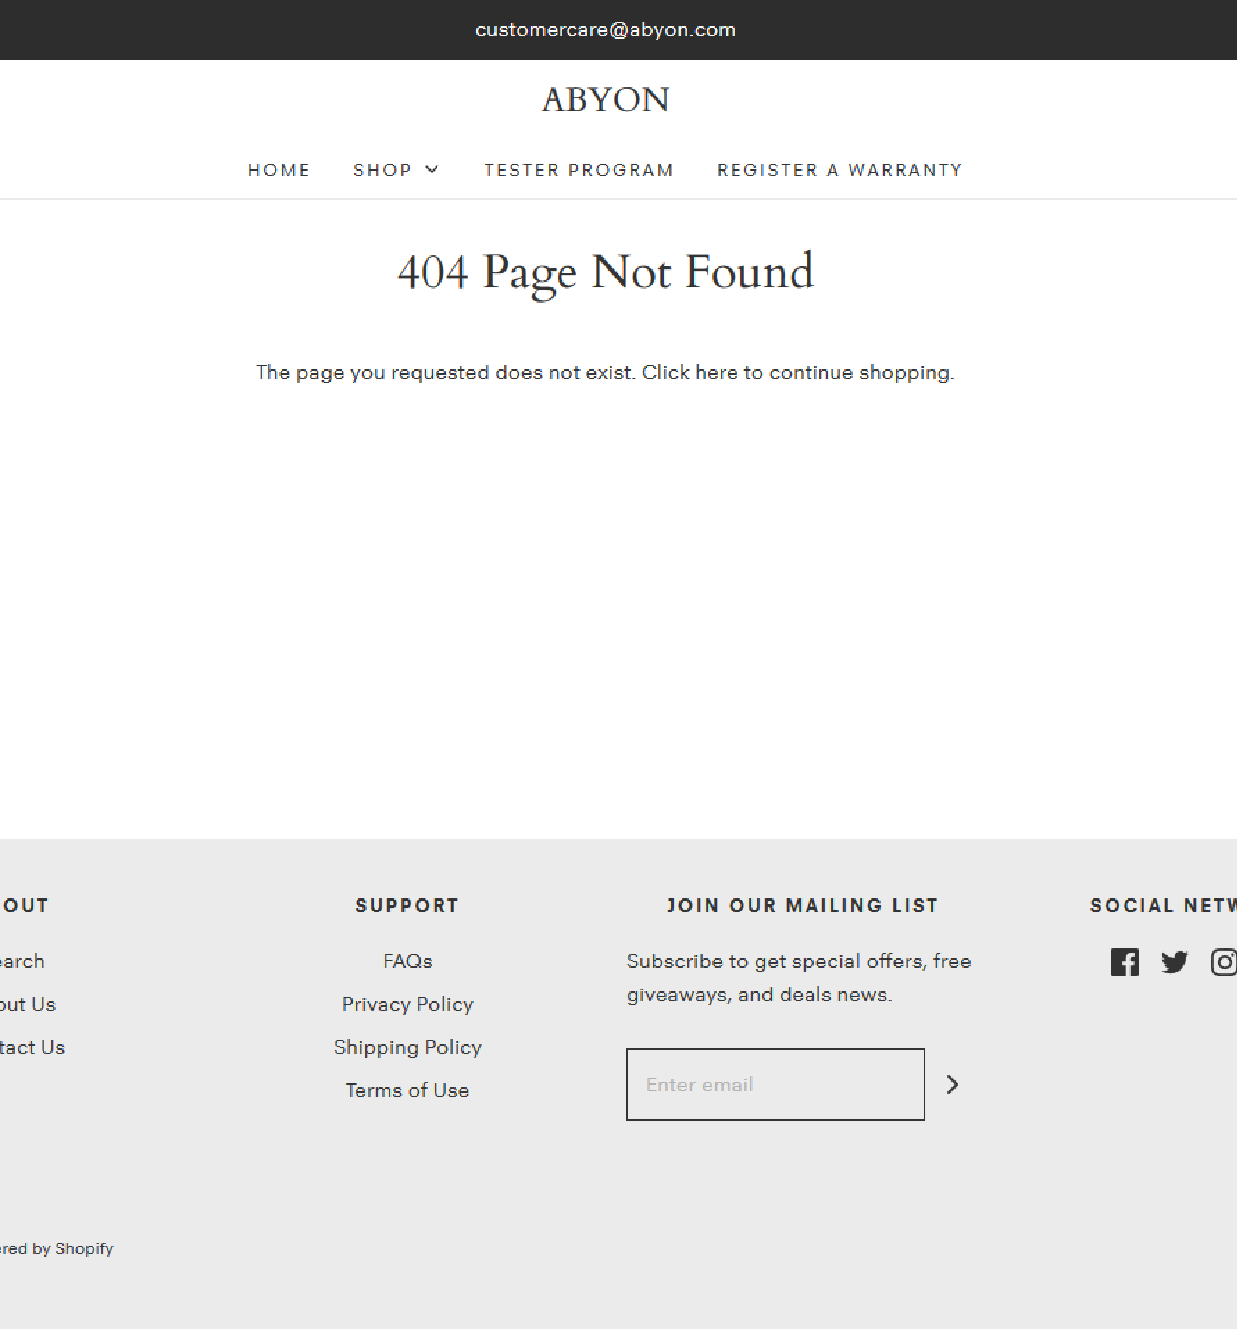
\includegraphics[width=.65\textwidth]{not_found1.pdf}}
    \vspace{-\baselineskip}
\end{figure}

Некоторые из производителей, которые не имеют собственного веб-сайта и политика безопасности которых не была найдена, пользуются услугами хостинга интернет-магазина непосредственно на Amazon. В таком случае, будучи частью интернет-магазина на них распространяется политика безопасности площадки, на которой они размещают свои предложения, причем политики могут различаться для разных стран.

\begin{figure}[H]
    \centering
    \ffigbox[\FBwidth]
    {\caption{Пример отсутствующей политики\label{fig:not_found2}}}
    {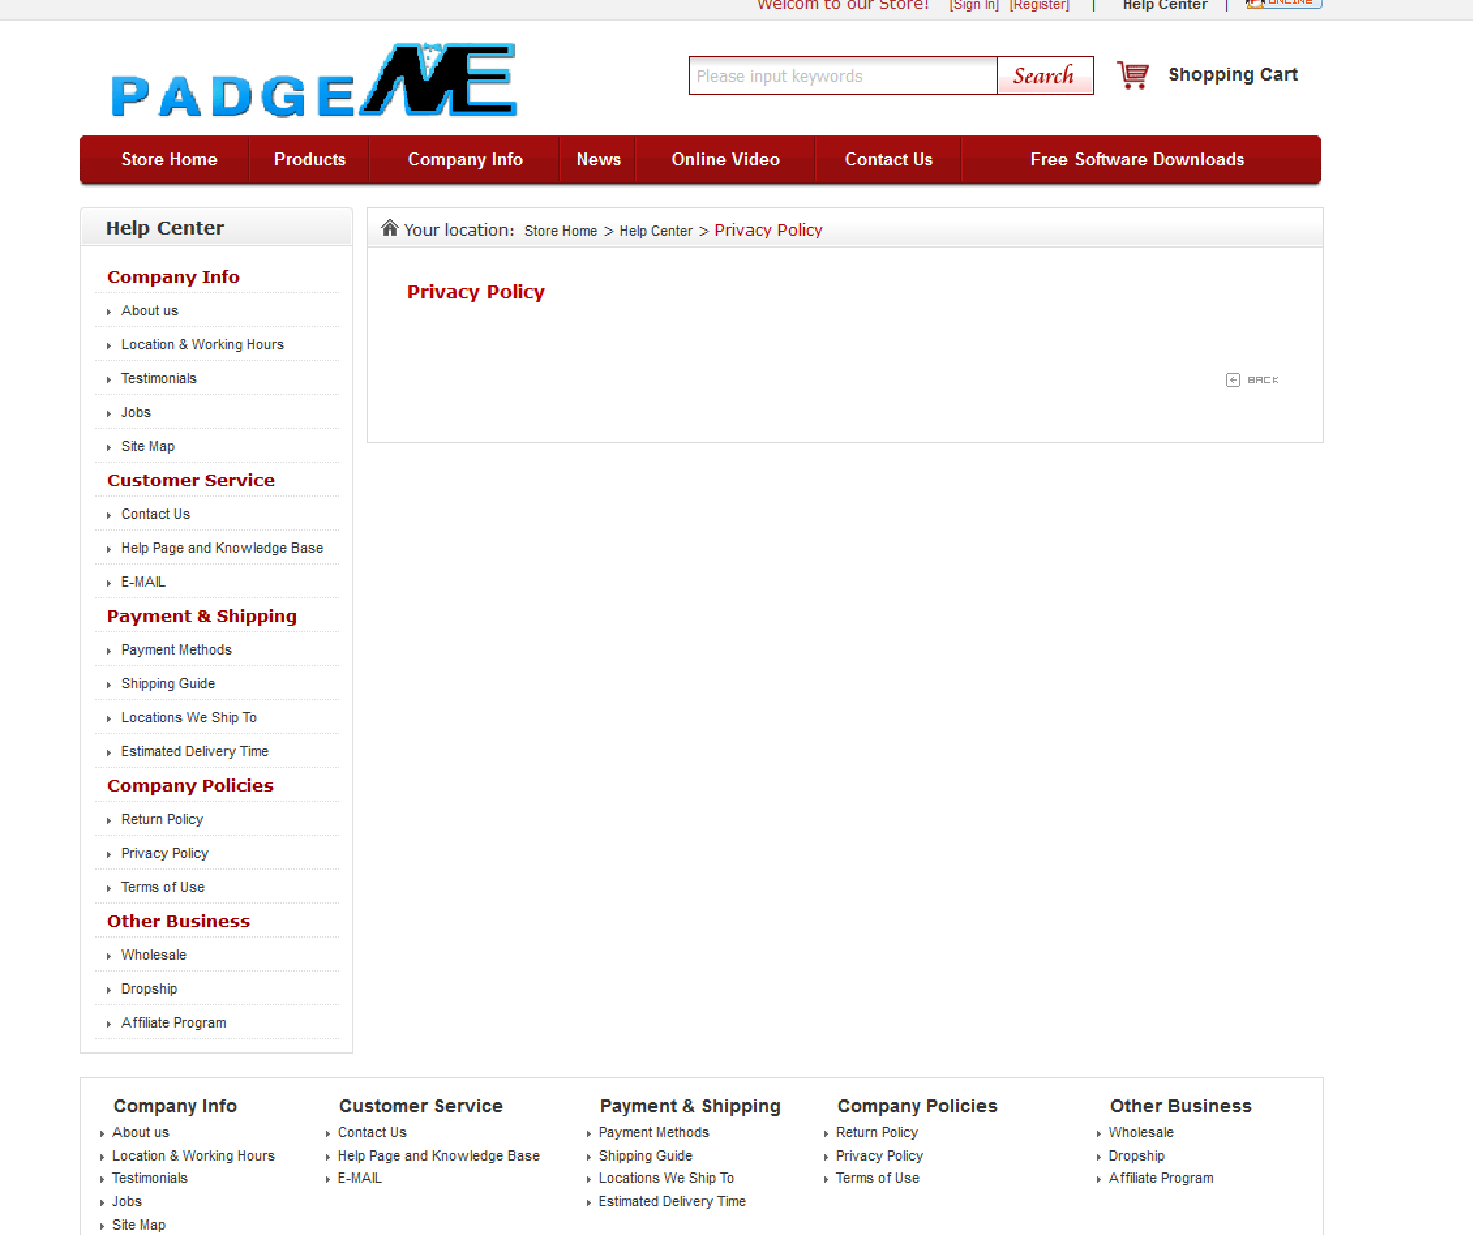
\includegraphics[width=.65\textwidth]{not_found2.pdf}}
    \vspace{-\baselineskip}
\end{figure}

 Случаи с использованием отдельных политик безопасности под различные типы устройств не были зафиксированы, хотя такие случаи и существуют, проще прибегнуть к явному заданию адресов политик, нежели чем к попытке автоматизировать процесс сбора, так как остаются непрозрачными способы выявления подобных ситуаций.

На рисунках \ref{fig:paragraph_size} и \ref{fig:policy_size} приведены статистические данные по объемам абзацев политик и самих документов соответственно.

\begin{figure}[H]
    \centering
    \ffigbox[\FBwidth]
    {\caption{Распределение политик по объему параграфа\label{fig:paragraph_size}}}
    {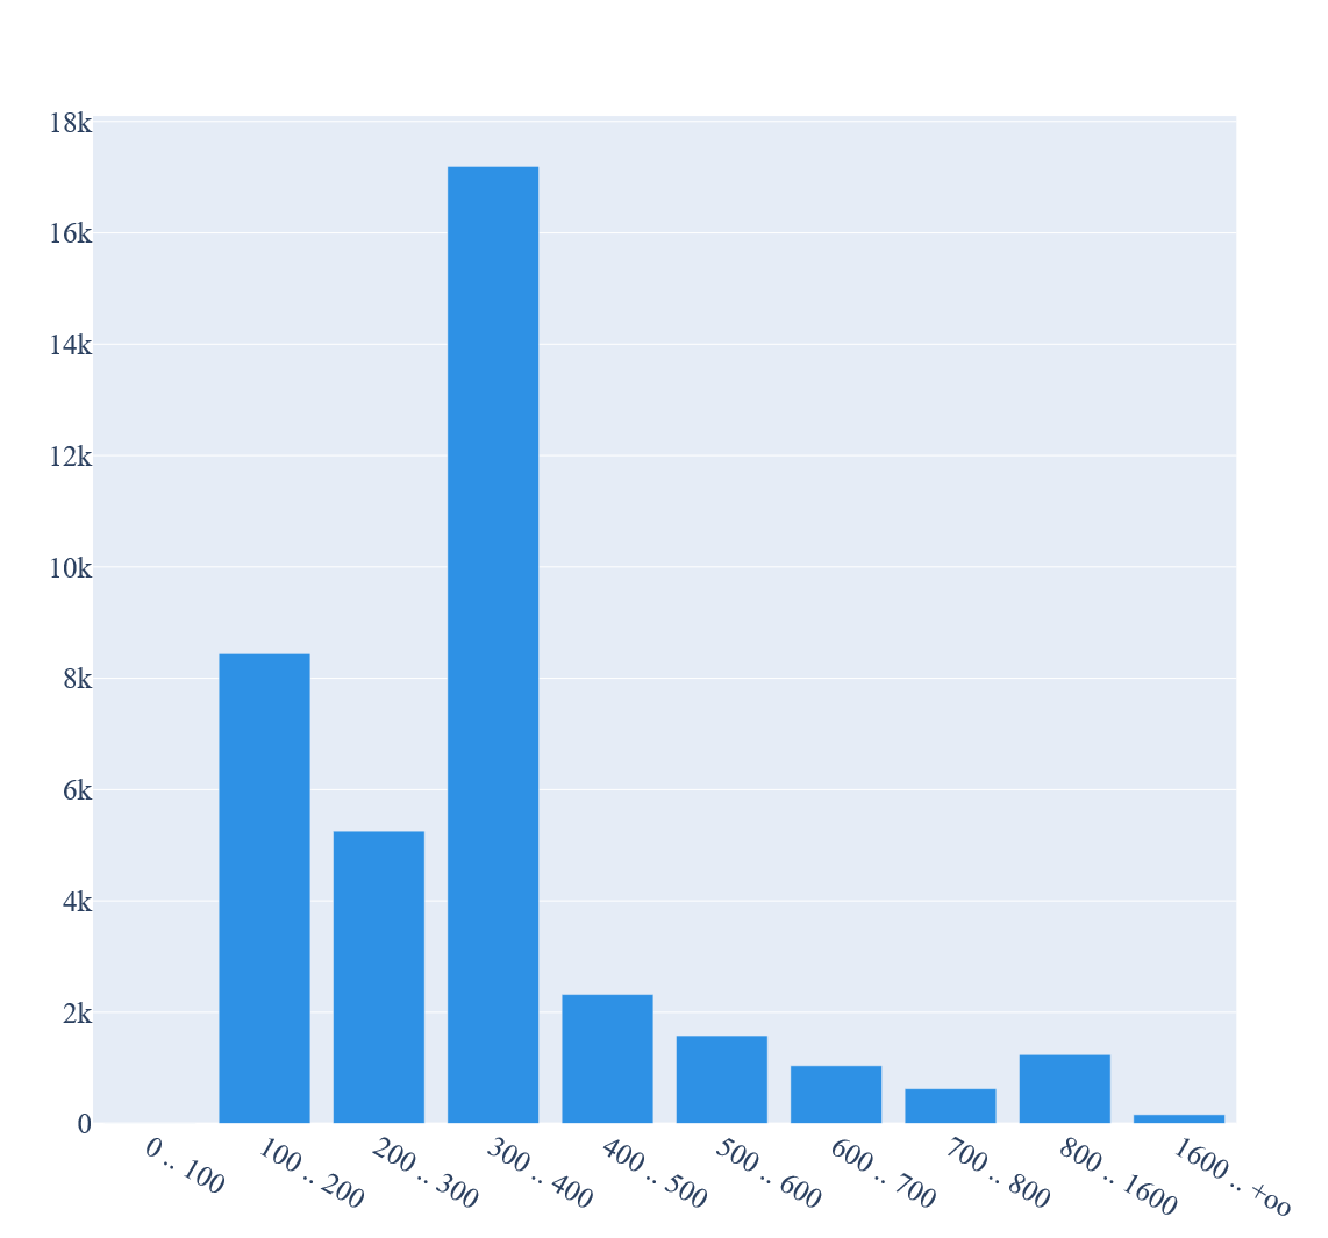
\includegraphics[width=.7\textwidth]{paragraph_size.pdf}}
    \vspace{-\baselineskip}
\end{figure}

\begin{figure}[H]
    \centering
    \ffigbox[\FBwidth]
    {\caption{Распределение политик по объему документа\label{fig:policy_size}}}
    {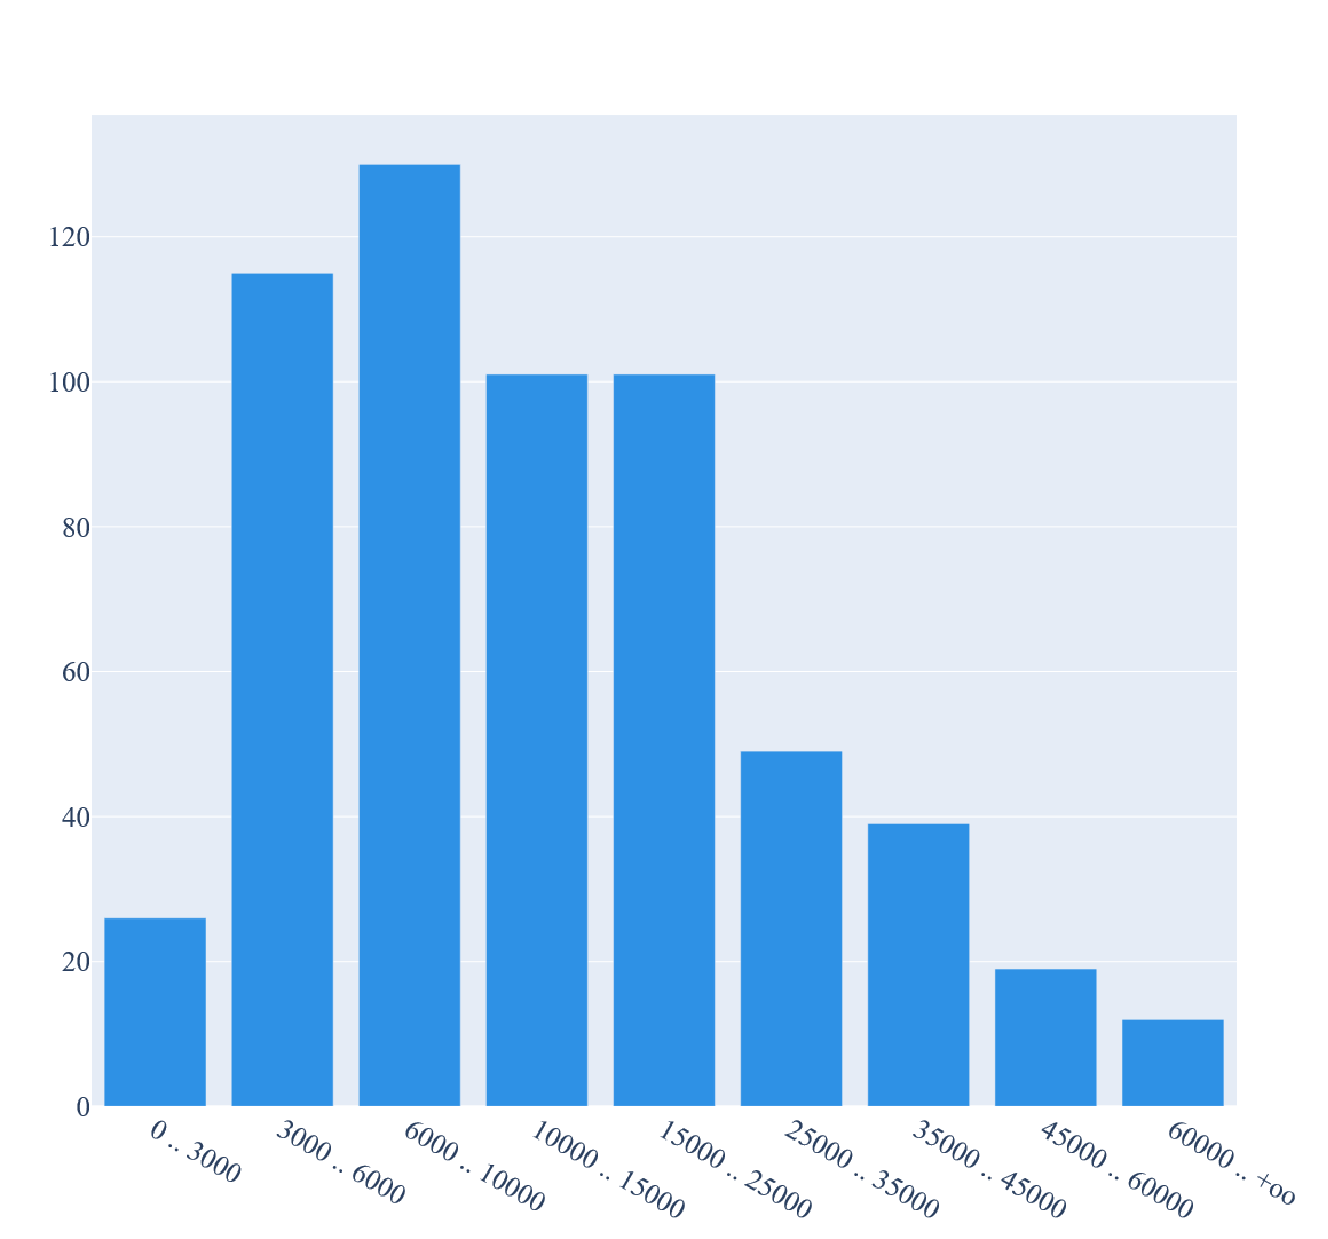
\includegraphics[width=.7\textwidth]{policy_size.pdf}}
    \vspace{-\baselineskip}
\end{figure}

Подсчет количества заголовков сложно организовать автоматизированно в связи с большим разнообразием html-разметки. На каждом сайте своя разметка, своя конвенция по нумерованию секций, заголовков, списков. На некоторых сайтах списки и заголовки нумеруются средствами html, на других нумерация проставлена вручную. Все это порождает разношерстность данных, и их обработка становится сложной с точки зрения учета всех возможных вариантов. Поэтому авторы решили прибегнуть к простому подсчету длин строк длиной меньше 100 символов и не содержащих при этом маркеров <<{list item}>>. Такой подход не даст очень точных показателей, но может дать приблизительные значения. На рисунках \ref{fig:structure_stats1} и \ref{fig:structure_stats2} приведена статистика по структурным элементам политик безопасности в двух частях. Здесь изображены детальные распределения структурных элементов для каждой из найденных политик безопасности.

\begin{figure}[H]
    \centering
    \ffigbox[\FBwidth]
    {\caption{Статистика первых 246 политик в IoT-датасете по структурным элементам\label{fig:structure_stats1}}}
    {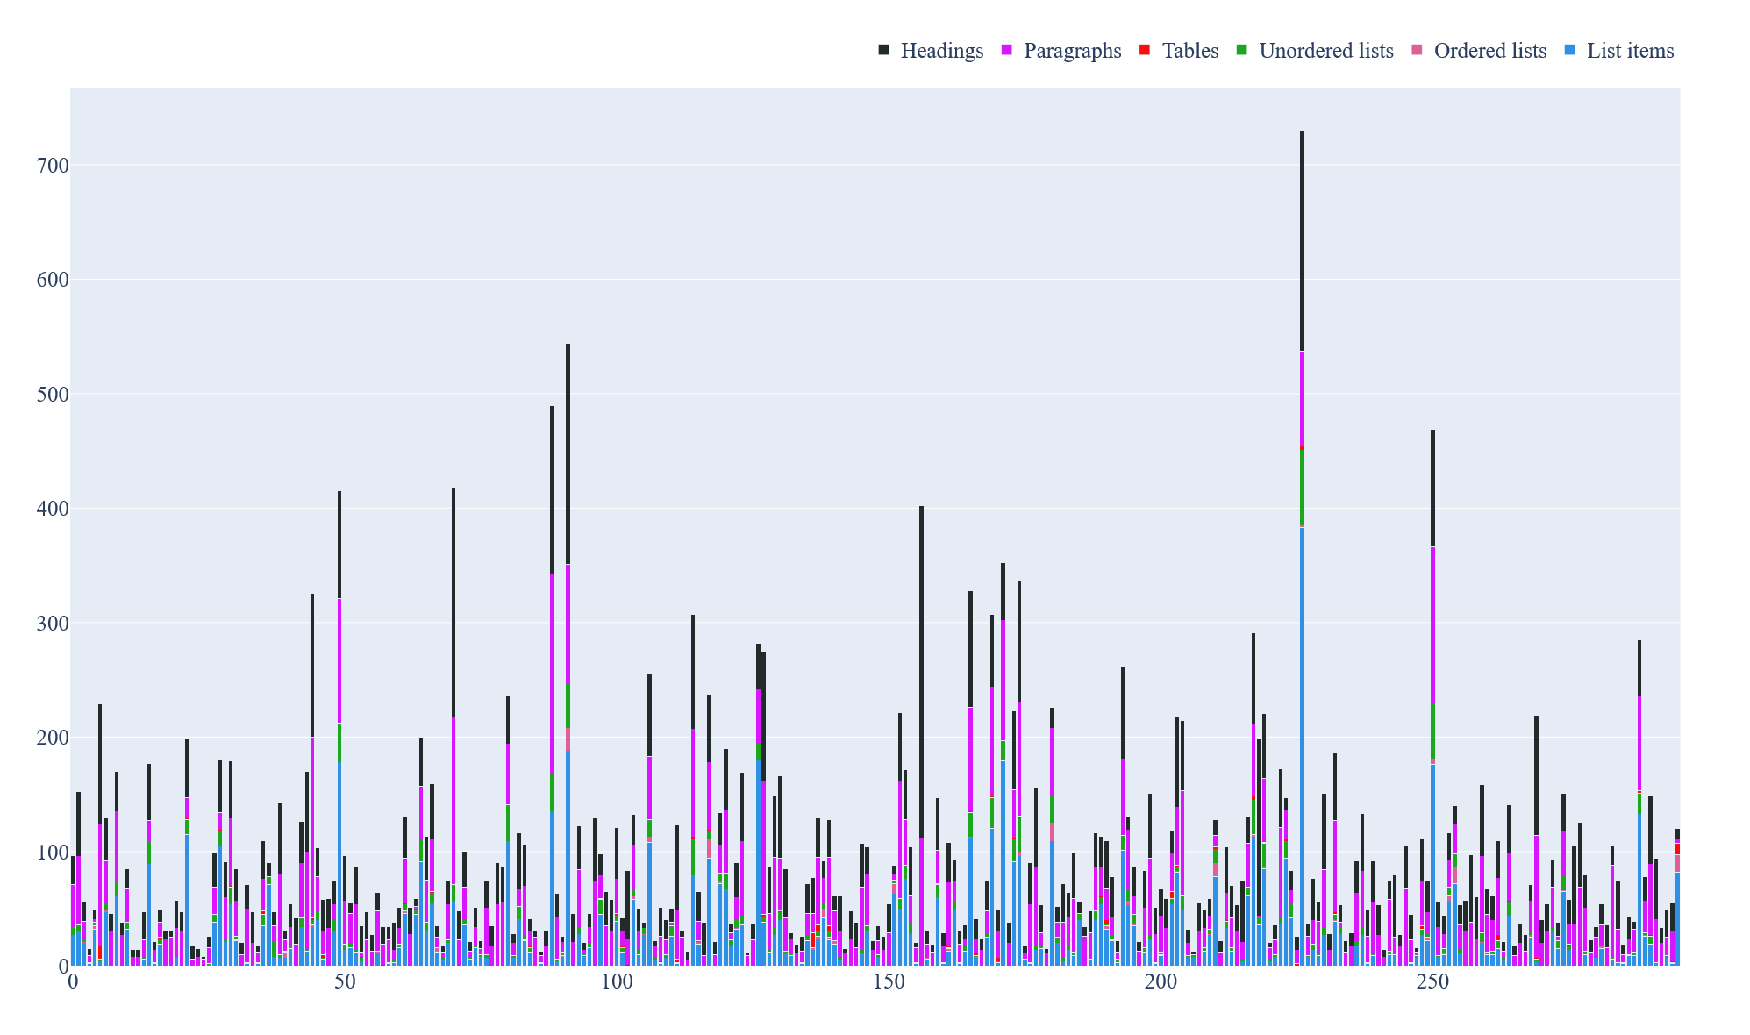
\includegraphics[width=\textwidth]{structure_stats1.pdf}}
    \vspace{-\baselineskip}
\end{figure}

\begin{figure}[H]
    \centering
    \ffigbox[\FBwidth]
    {\caption{Статистика последних 246 политик в IoT-датасете по структурным элементам\label{fig:structure_stats2}}}
    {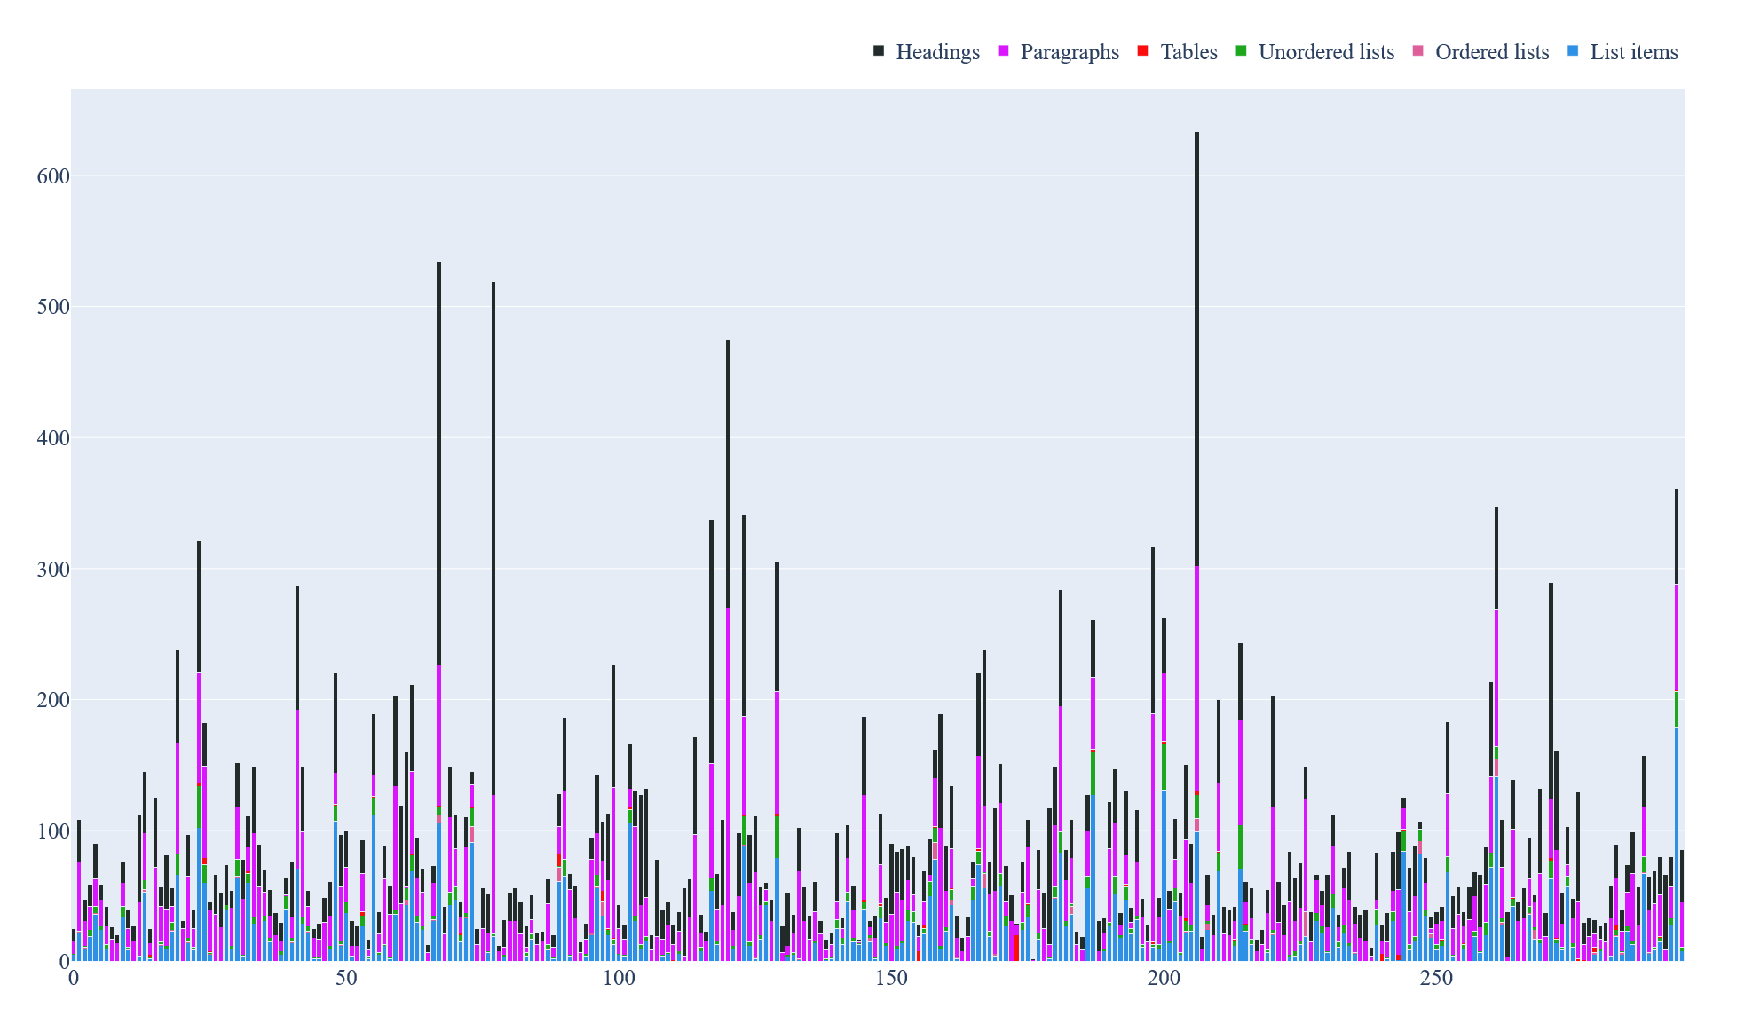
\includegraphics[width=\textwidth]{structure_stats2.pdf}}
    \vspace{-\baselineskip}
\end{figure}

Таким образом можно описать среднестатистическую политику безопасности, которая состоит из 31.5 абзацев, 33 заголовков, 23.6 элементов перечислений, 0.7 нумерованных списков, 4.4 ненумерованных списка, 0.5 таблиц.

Для дополнительного статистического анализа датасета, он был кластеризован с помощью латентного размещения Дирихле. Как и в предыдущих разделах для кластеризации политики безопасности были разбиты на абзацы, после чего была проведена предобработка, состоящая из лемматизации, удаления пунктуации и так называемых стоп-слов. В таблице \ref{tab:iot_clusters} приведены результаты моделирования тем в IoT-датасете. В предыдущих разделах уже была исследована точность латентного размещения Дирихле, его преимущества и недостатки, на основании чего IoT-датасет был проанализирован именно таким способом. По результатам видно, что с помощью такой кластеризации можно выделить различные аспекты политик безопасности.

\begin{ltwrap}{2mm}{1}{\footnotesize}
    \begin{longtable}[H]{|C{.05\x}|M{.475\x}|M{.475\x}|}
        \caption{Тематическое моделирование\label{tab:iot_clusters}}\\\hline
        \multicolumn{1}{|H{.05\x}|}{№}
        & \multicolumn{1}{H{.475\x}|}{Координаты семантического пространства} 
        & \multicolumn{1}{H{.475\x}|}{Возможные сценарии использования}\\\hline
        \endfirsthead
        \caption*{Продолжение таблицы \ref{tab:iot_clusters}}\\\hline
        \multicolumn{1}{|H{.05\x}|}{№}
        & \multicolumn{1}{H{.475\x}|}{Координаты семантического пространства} 
        & \multicolumn{1}{H{.475\x}|}{Возможные сценарии использования}\\\hline
        \endhead
        \endfoot
        \endlastfoot
        0 & email, send, promotional, communication, marketing, opt, product, service, message, list & First-party collection, Opt-in, opt-out messages and notifications to end user \\\hline
        1 & party, third, service, information, privacy, website, share, policy, site, advertising & Third parties sharing for marketing purposes \\\hline
        2 & removed, href, hyperref, question, contact, privacy, us, please, policy, comment & Contact information: company \\\hline
        3 & cookie, device, browser, service, address, website, site, collect, information, use & First-party collection: browser and device information \\\hline
        4 & child, age, entering, detection, year, fill, redirected, show, knowingly & Special audience: children \\\hline
        5 & sensor, educational, suggestion, top, acquirer, mailing, employment, job, taking, clickstream & First-party collection: device and service specific information \\\hline
        6 & corporate, automated, storefrontdigest, indefinite, personalization, direction, administrator, token, shop, employed & Other \\\hline
        7 & data, personal, right, request, processing, information, necessary, legal, purpose, law & First-party collection: right to edit, access, with specified (legal) basis of data processing \\\hline
        8 & sponsor, push, reply, default, swiss, desire, becoming, correspondence, calling, representative & Other \\\hline
        9 & asset, service, product, merger, company, item, list, business, another, referral & Third-party sharing in case of company acquisition and merging \\\hline
        10 & erasure, unaffiliated, input, approximate, format, appliance, pref, persistent, canadian, short & Right to erase \\\hline
        11 & address, name, information, account, email, promotion, password, u, collect, contact & First-party collection: personal and account information \\\hline
        12 & security, protect, safety, hosted, secure, violate, property, others, technical, law & Data security \\\hline
        13 & california, state, resident, institution, law, united, ccpa, right, request, country & Special audience: California residents \\\hline
        14 & change, policy, privacy, statement, time, notice, pci, payment, ds, update & Privacy policy changes \\\hline
    \end{longtable}
\end{ltwrap}

При кластеризации порог аффилиации абзаца политики безопасности был установлен в 0.3, параграф относился к нескольким кластерам, если вероятность аффилиации с ним была больше указанного порога. По графику на рисунке \ref{fig:topics_stats} можно судить, какую часть от общего объема текстов занимают те или иные аспекты политик безопасности.

\begin{figure}[H]
    \centering
    \ffigbox[\FBwidth]
    {\caption{Статистика аспектов в IoT-датасете\label{fig:topics_stats}}}
    {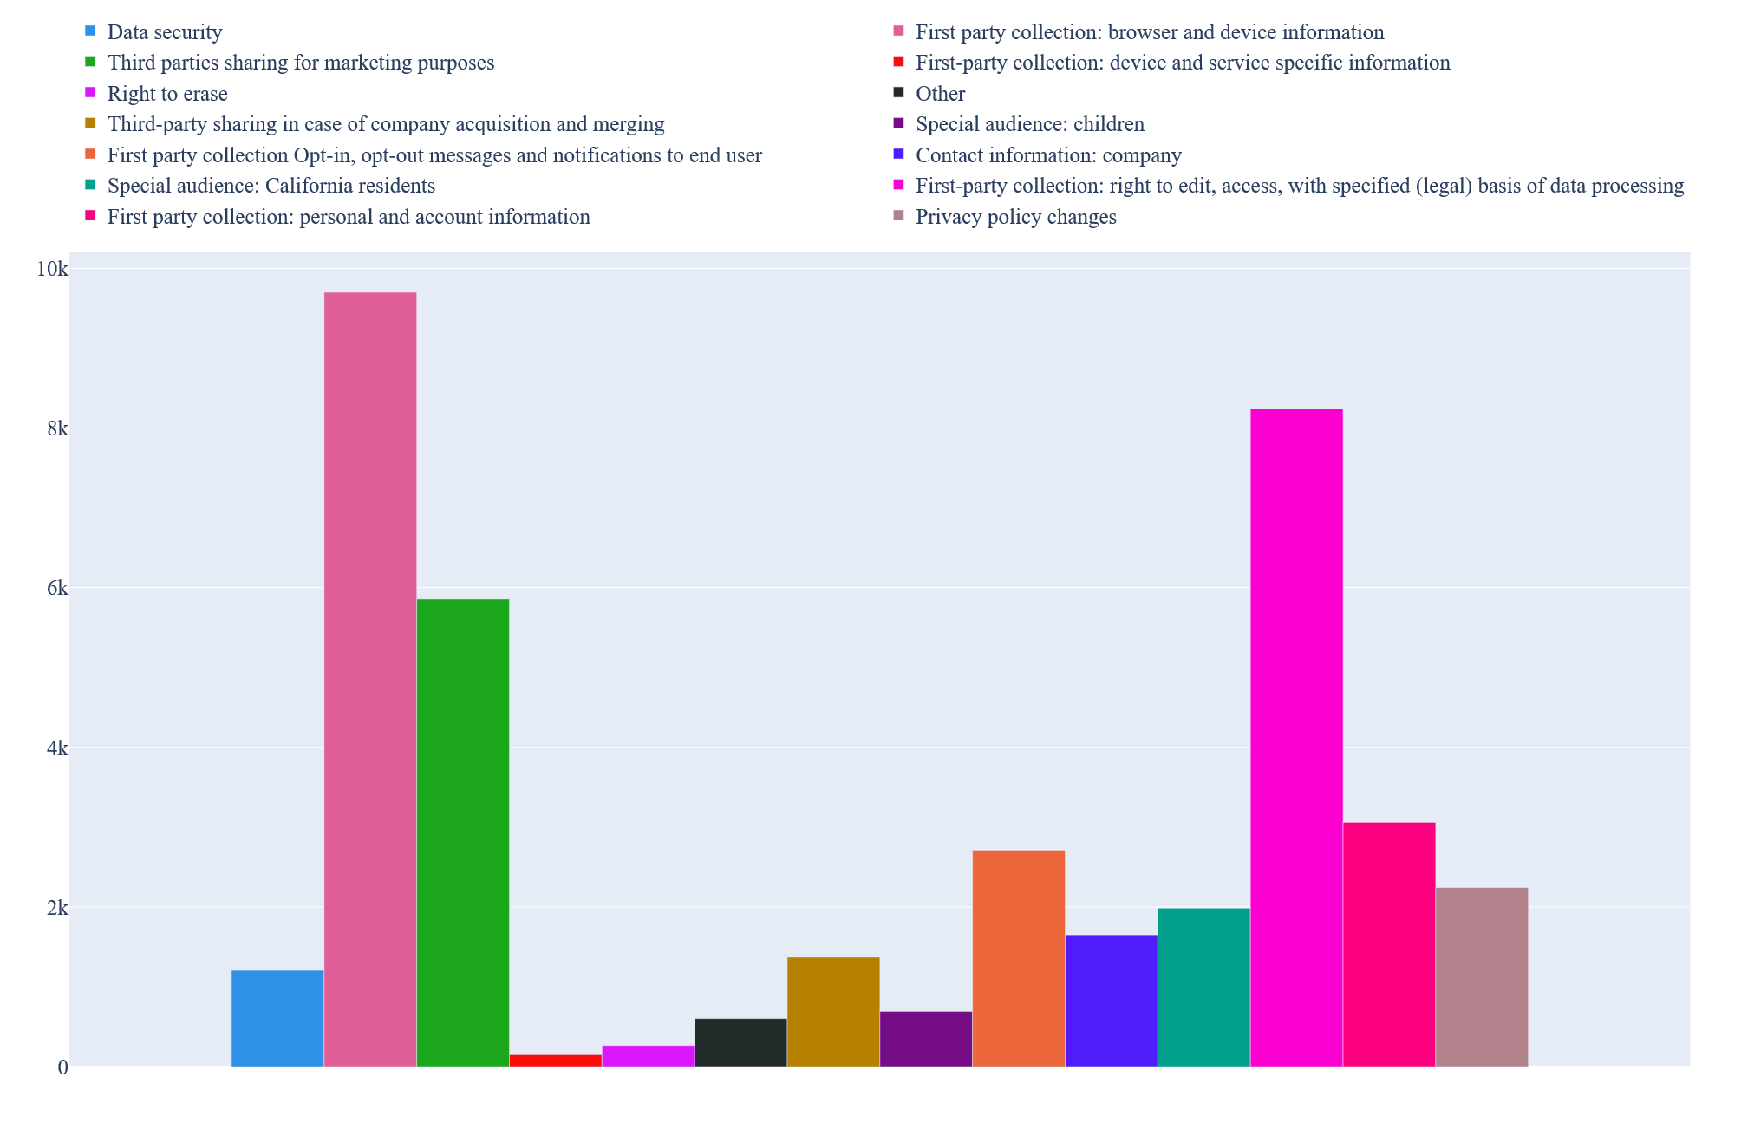
\includegraphics[width=.8\textwidth]{topics_stats.pdf}}
    \vspace{-\baselineskip}
\end{figure}

Как заключение статистического обзора сформированного датасета на рисунках \ref{fig:topics_stats1} и \ref{fig:topics_stats2} приведено детальное распределение аспектов политик безопасности по каждой конкретной политике.

\begin{figure}[H]
    \centering
    \ffigbox[\FBwidth]
    {\caption{Статистика первых 246 политик в IoT-датасете по аспектам\label{fig:topics_stats1}}}
    {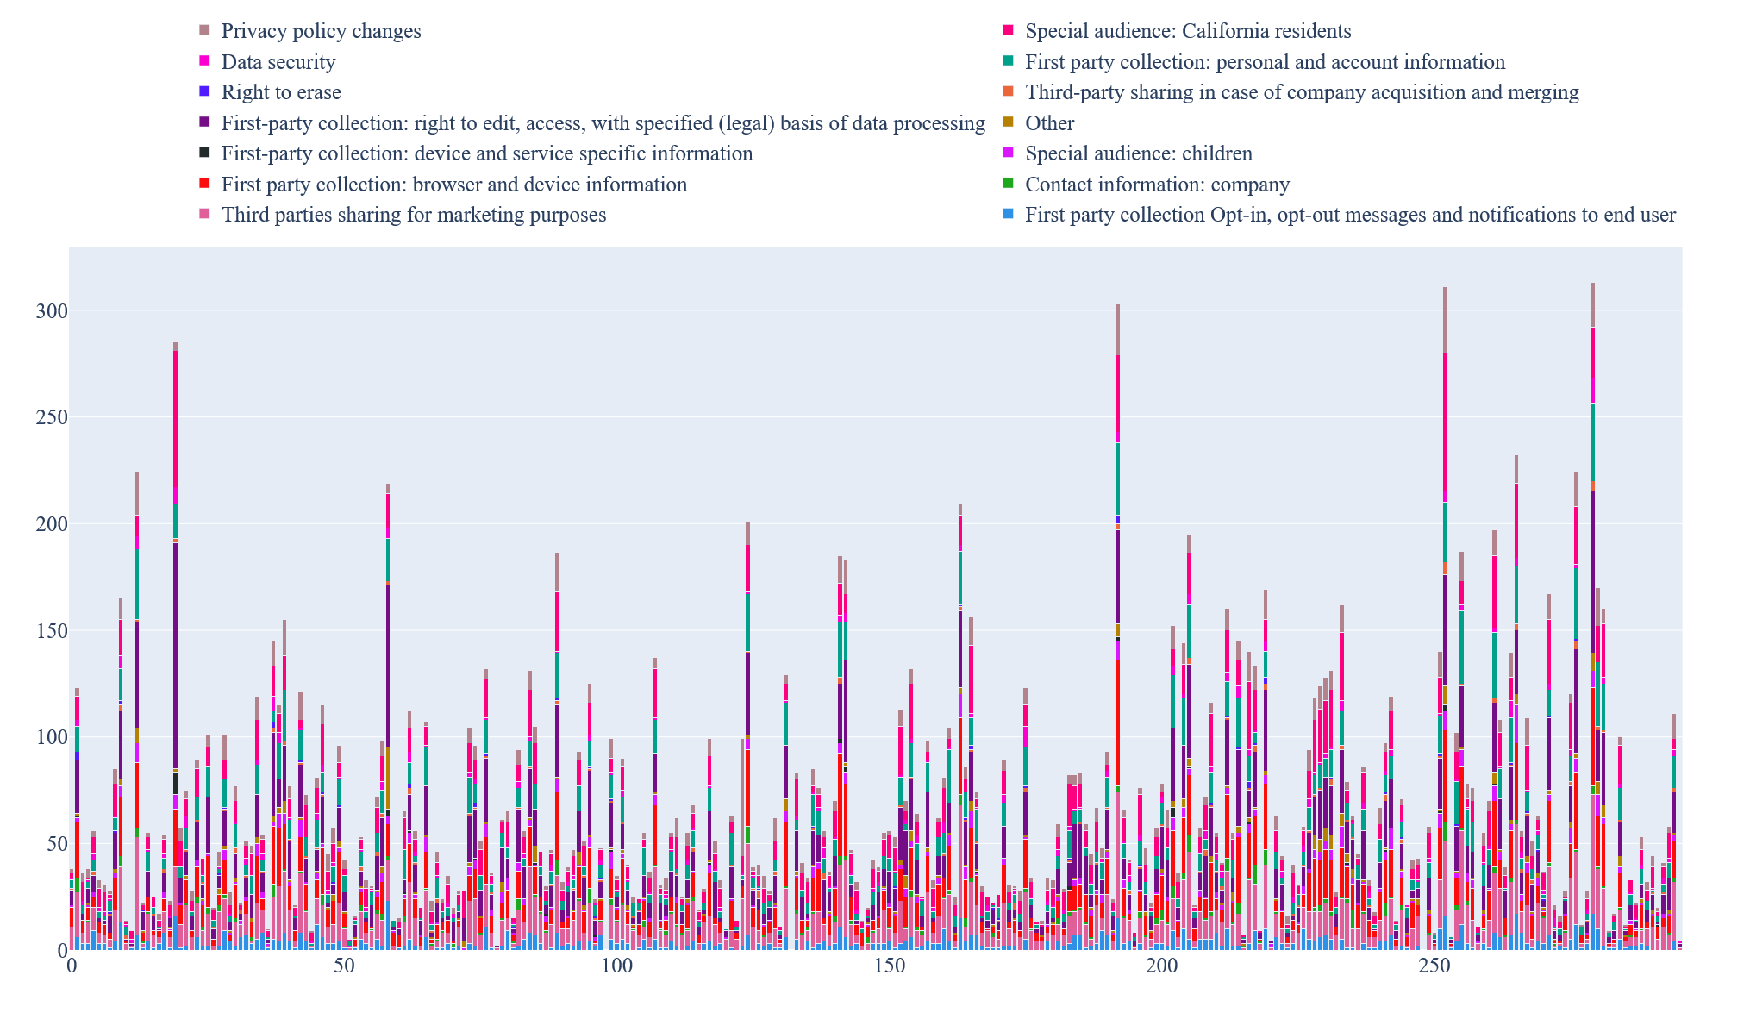
\includegraphics[width=\textwidth]{topics_stats1.pdf}}
    \vspace{-\baselineskip}
\end{figure}

\begin{figure}[H]
    \centering
    \ffigbox[\FBwidth]
    {\caption{Статистика последних 246 политик в IoT-датасете по аспектам\label{fig:topics_stats2}}}
    {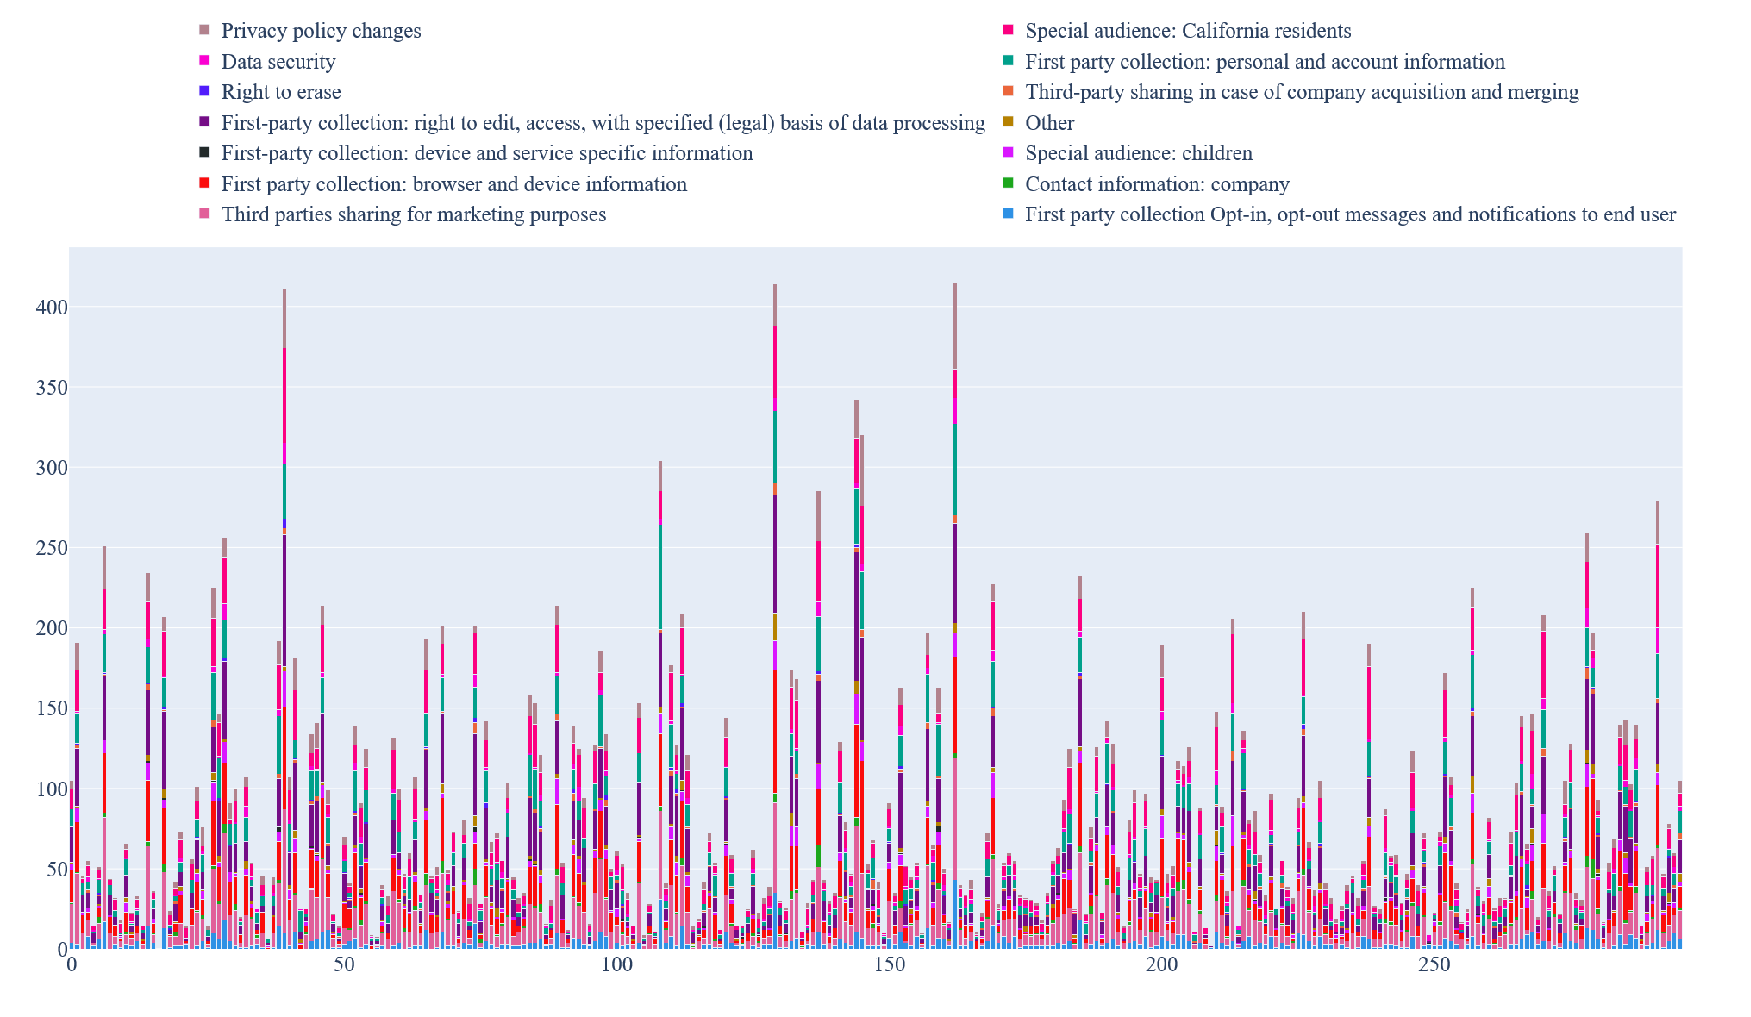
\includegraphics[width=\textwidth]{topics_stats2.pdf}}
    \vspace{-\baselineskip}
\end{figure}

Здесь в виде гистограммы представлены распределения всех 15 аспектов, выделенных алгоритмом LDA. Каждый абзац может относиться к нескольким аспектам с порогом аффилиации 0.3.

\subsection{Применение инструмента разметки данных}
\label{sec:real_proto}

В ходе реализации был разработан инструмент разметки датасета. На рисунках \ref{fig:init_annotation}--\ref{fig:result2} представлен его конечный вид. В качестве тестового примера была взята часть онтологии, предложенной в \cite{P2Onto}, и посвященной описанию активности по отношению к персональным данным. Инструмент был настроен для работы с указанной частью онтологии. Выделения и нанесенная разметка в данных примерах не являются осмысленными и выполнялись исключительно с целью демонстрации работоспособности приложения.

На рисунке \ref{fig:init_annotation} представлено начальное состояние страницы разметки. В начальном состоянии панель инструментов не показывает ни одного слоя, текст для разметки представлен в первоначальном виде.

На рисунке \ref{fig:selection} представлена реакция инструмента на выделение текста пользователем. При выделении пользователем текста на панели слоев закрепляются слои доступные для наложения, выбранные контекстуально, в соответствии с настроенной иерархией разметки.
\begin{figure}[H]
    \centering
    \ffigbox[\FBwidth]
    {\caption{Начальное состояние страницы разметки\label{fig:init_annotation}}}
    {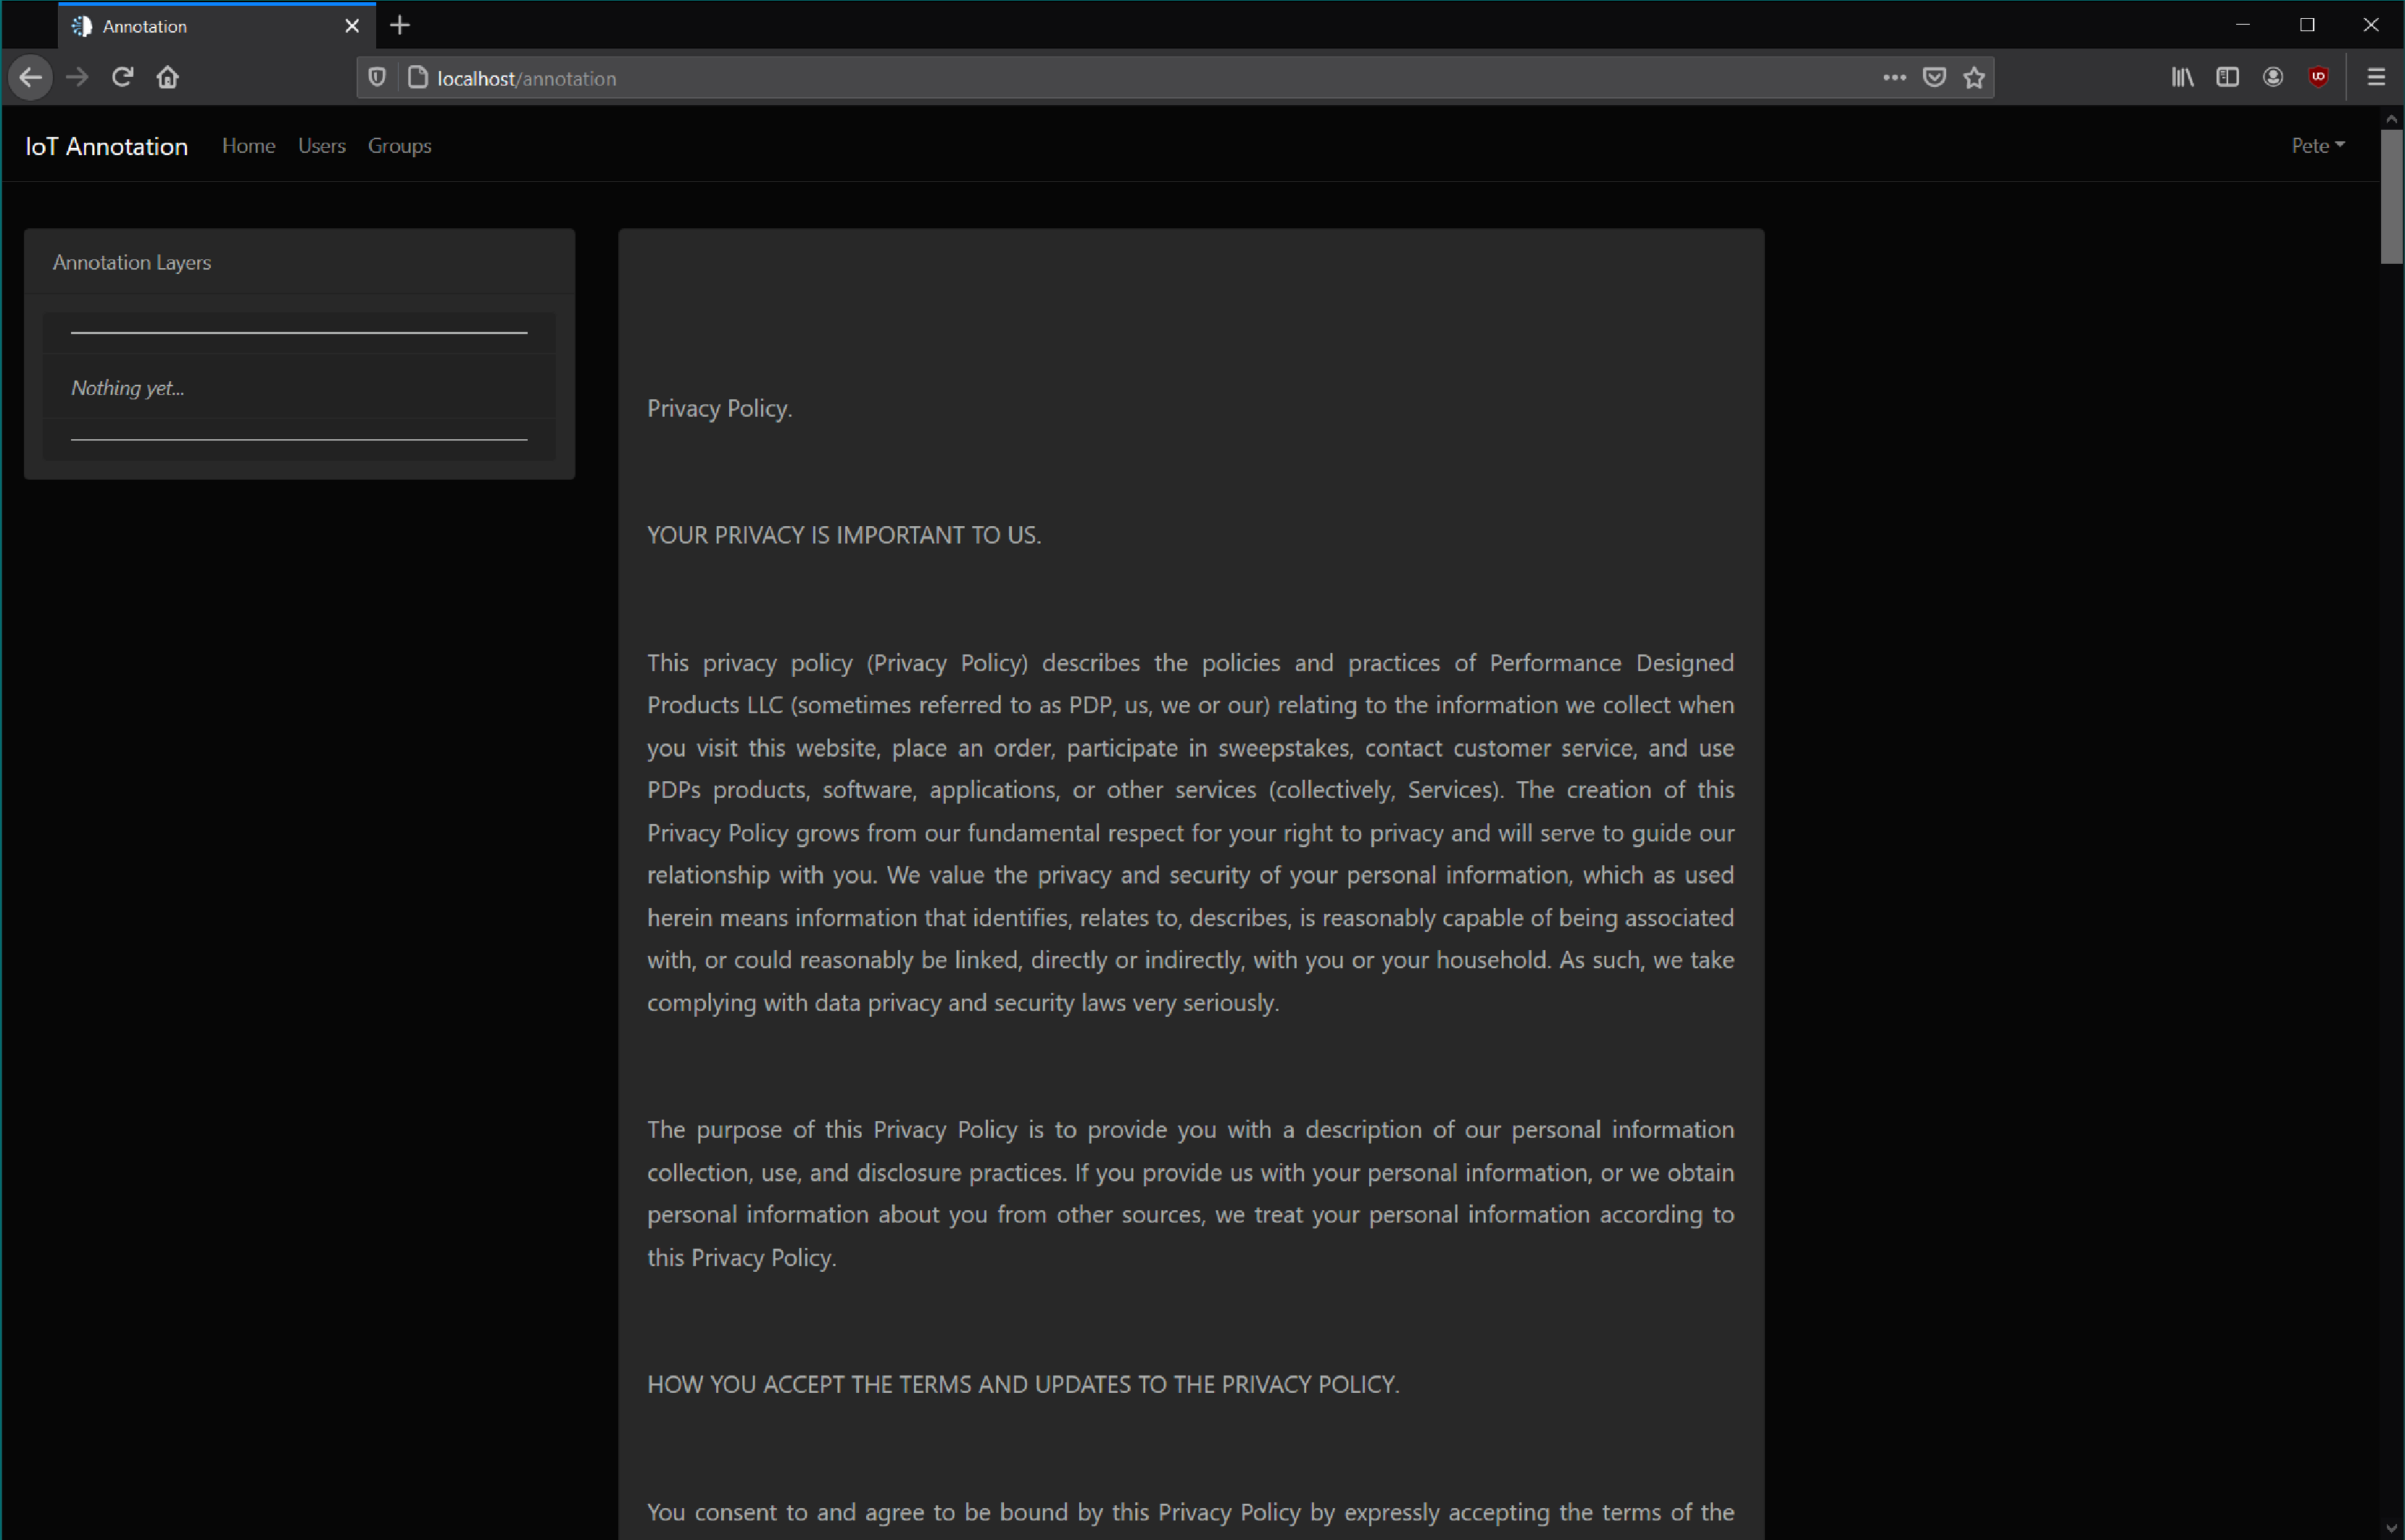
\includegraphics[width=.8\textwidth]{init_annotation.pdf}}
    \vspace{-\baselineskip}
\end{figure}
\begin{figure}[H]
    \centering
    \ffigbox[\FBwidth]
    {\caption{Выделение текста\label{fig:selection}}}
    {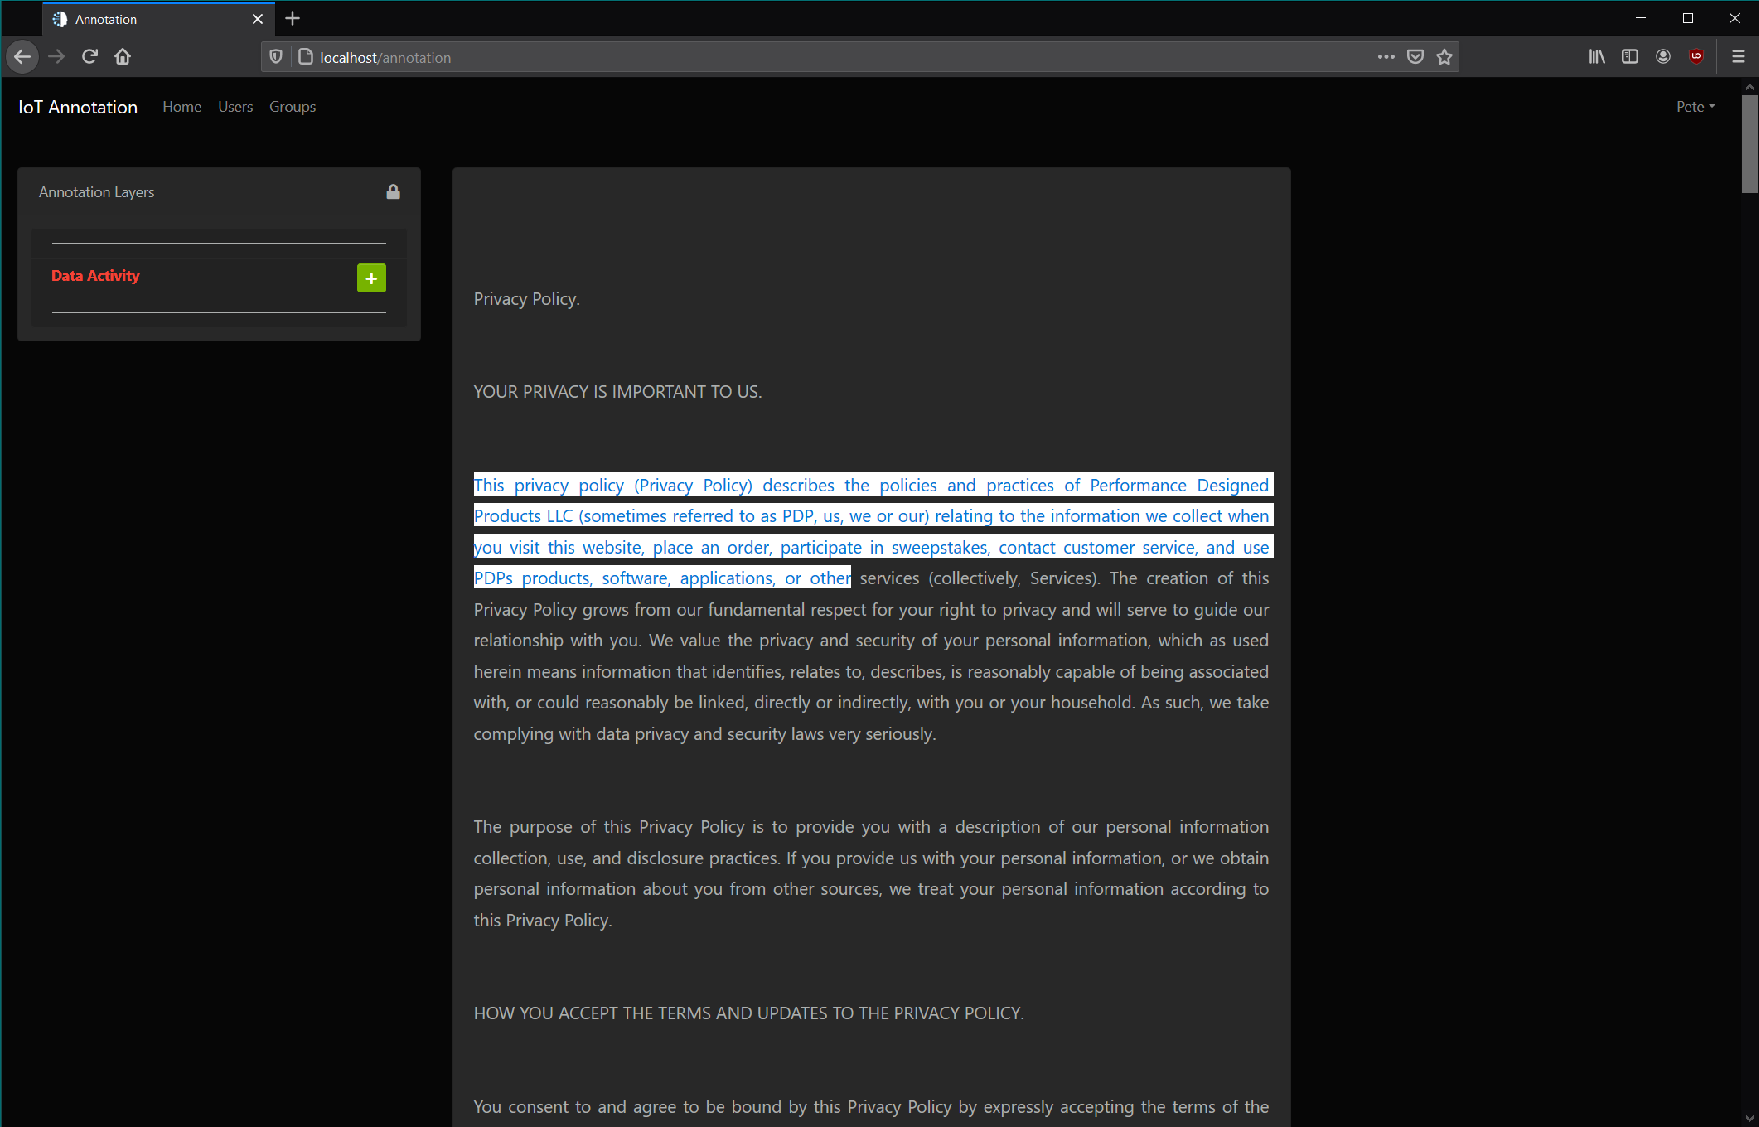
\includegraphics[width=.8\textwidth]{selection.pdf}}
    \vspace{-\baselineskip}
\end{figure}

На рисунке \ref{fig:annotated1} представлено состояние страницы разметки после нанесения слоя разметки. Теперь панель слоев отображает текущие наложенные слои для элемента, на который наведен указатель мыши.
\begin{figure}[H]
    \centering
    \ffigbox[\FBwidth]
    {\caption{Нанесение слоя разметки\label{fig:annotated1}}}
    {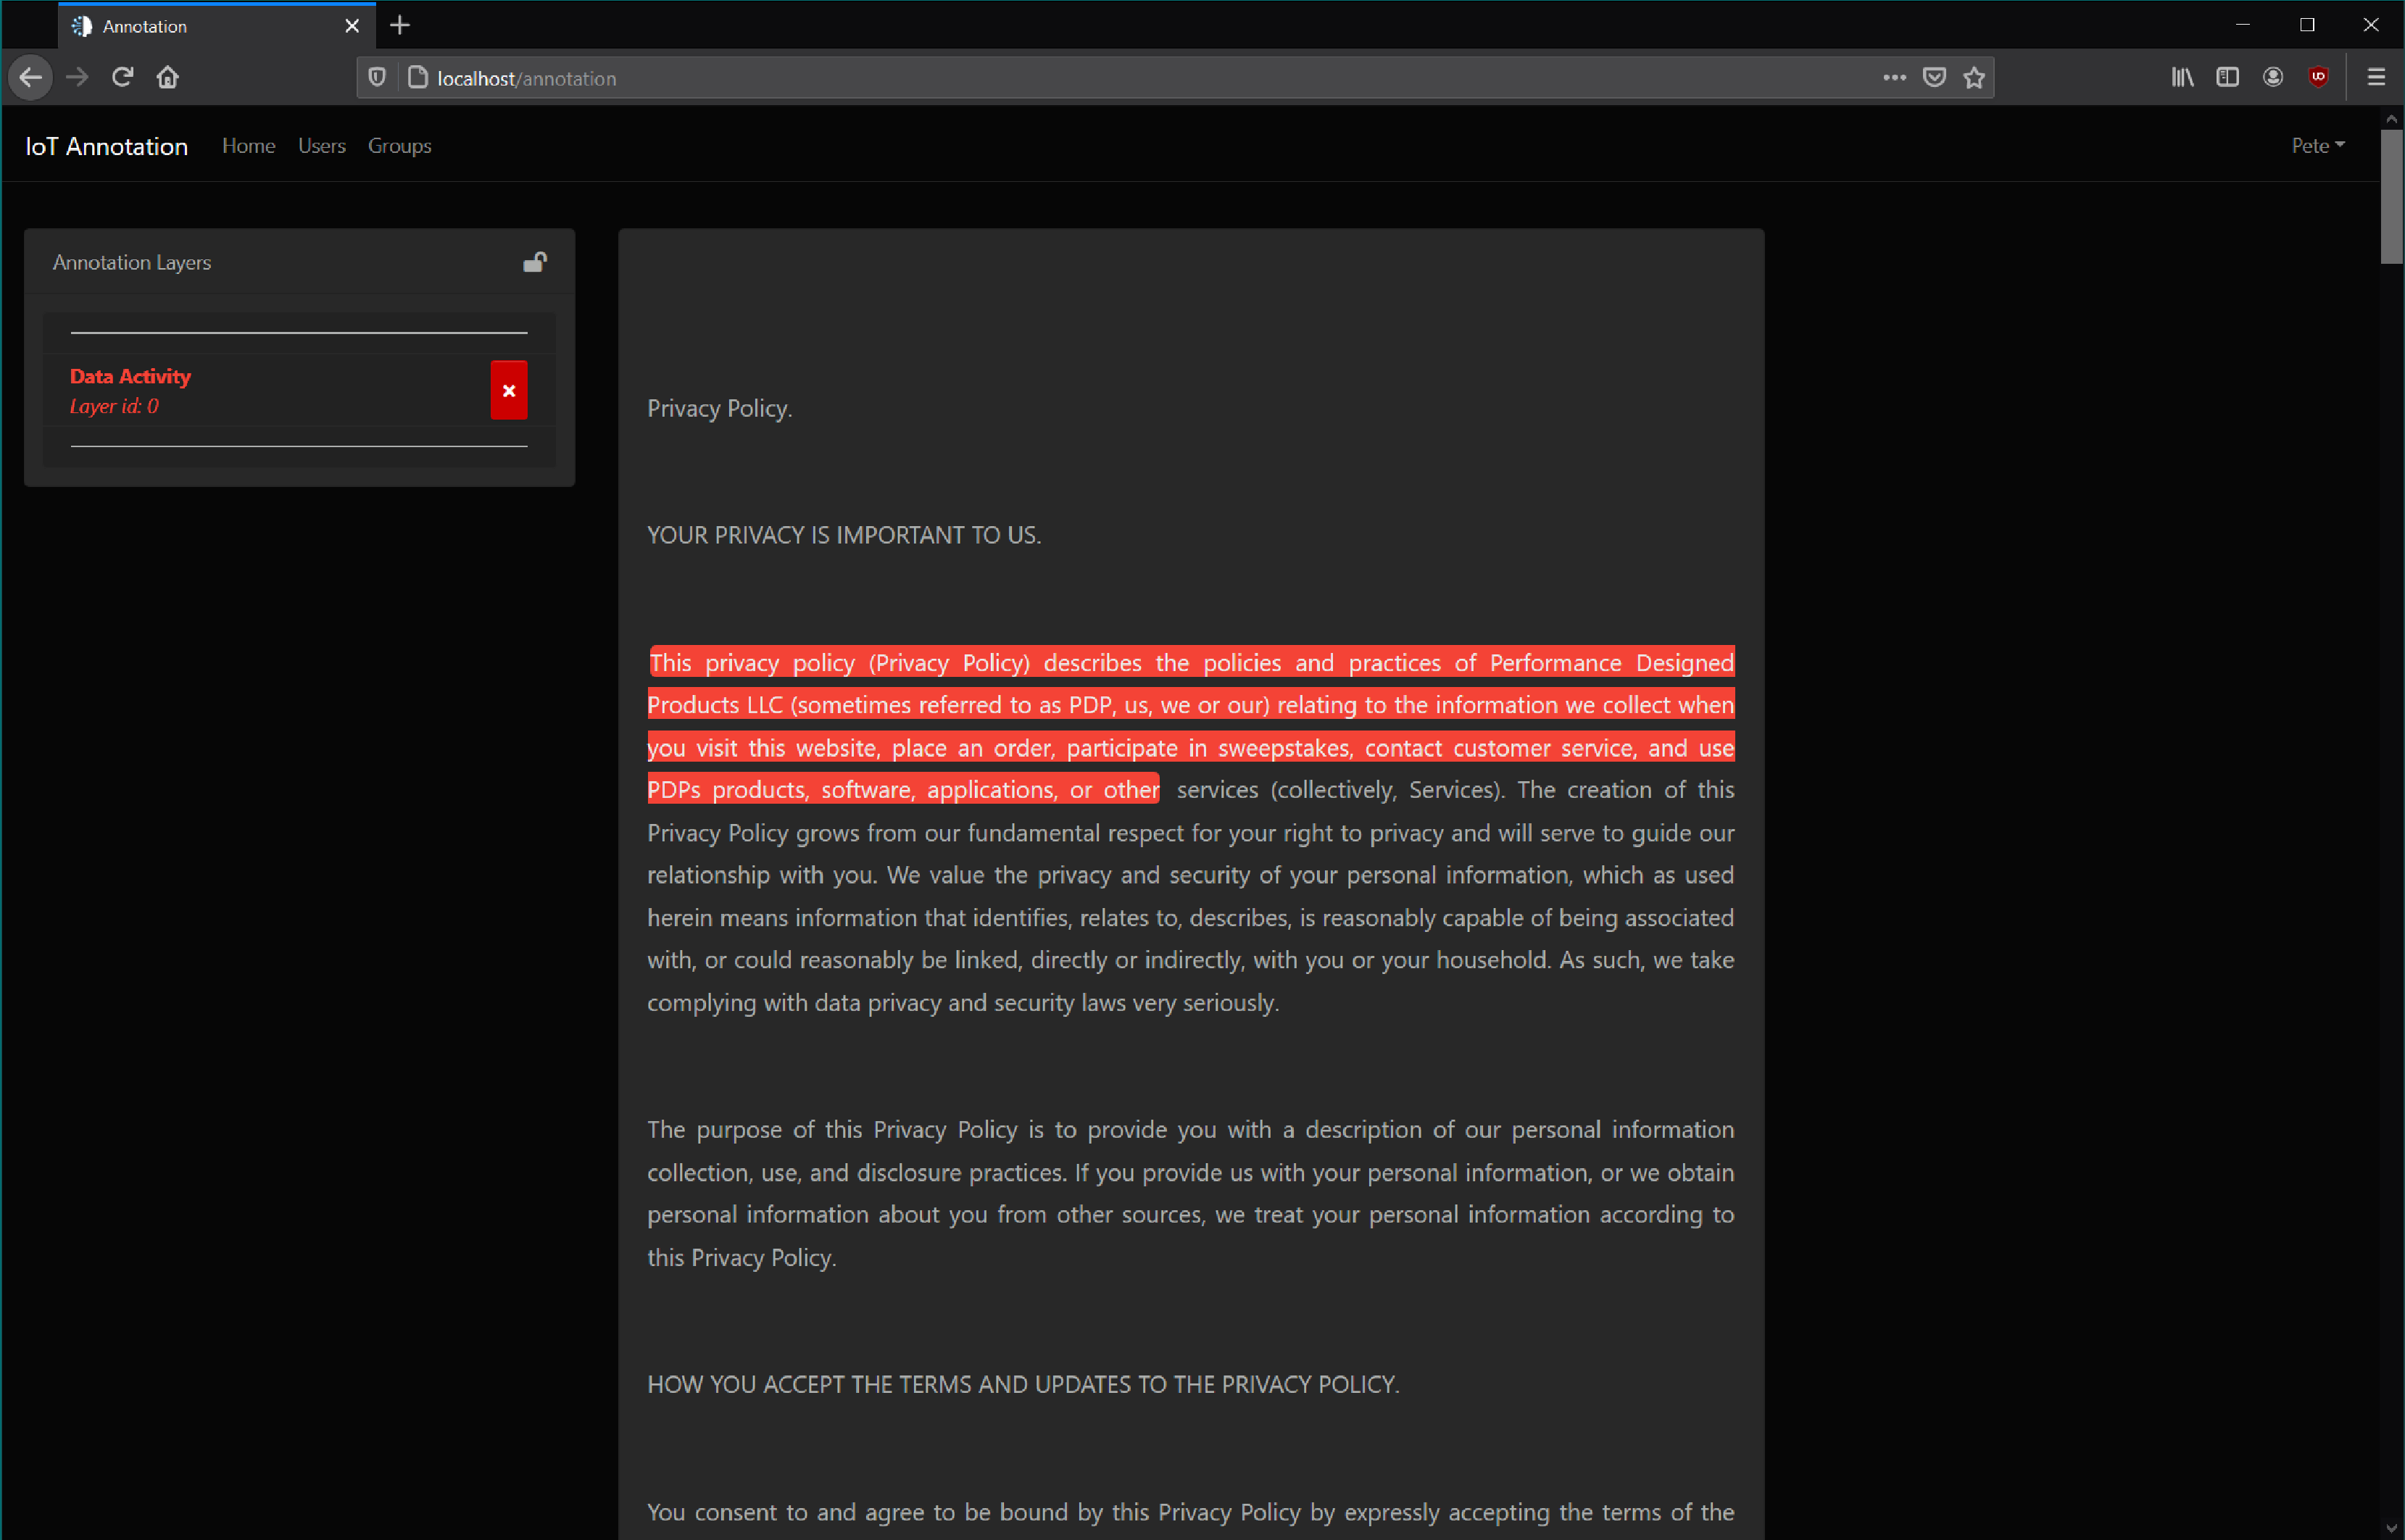
\includegraphics[width=.8\textwidth]{annotated1.pdf}}
    \vspace{-\baselineskip}
\end{figure}

На рисунке \ref{fig:selection2} представлена реакция инструмента на выделение текста пользователем. Теперь контекстуально на основе информации о наложенных слоях, предлагаются слои другого уровня детализации.
\begin{figure}[H]
    \centering
    \ffigbox[\FBwidth]
    {\caption{Выделение размеченного текста\label{fig:selection2}}}
    {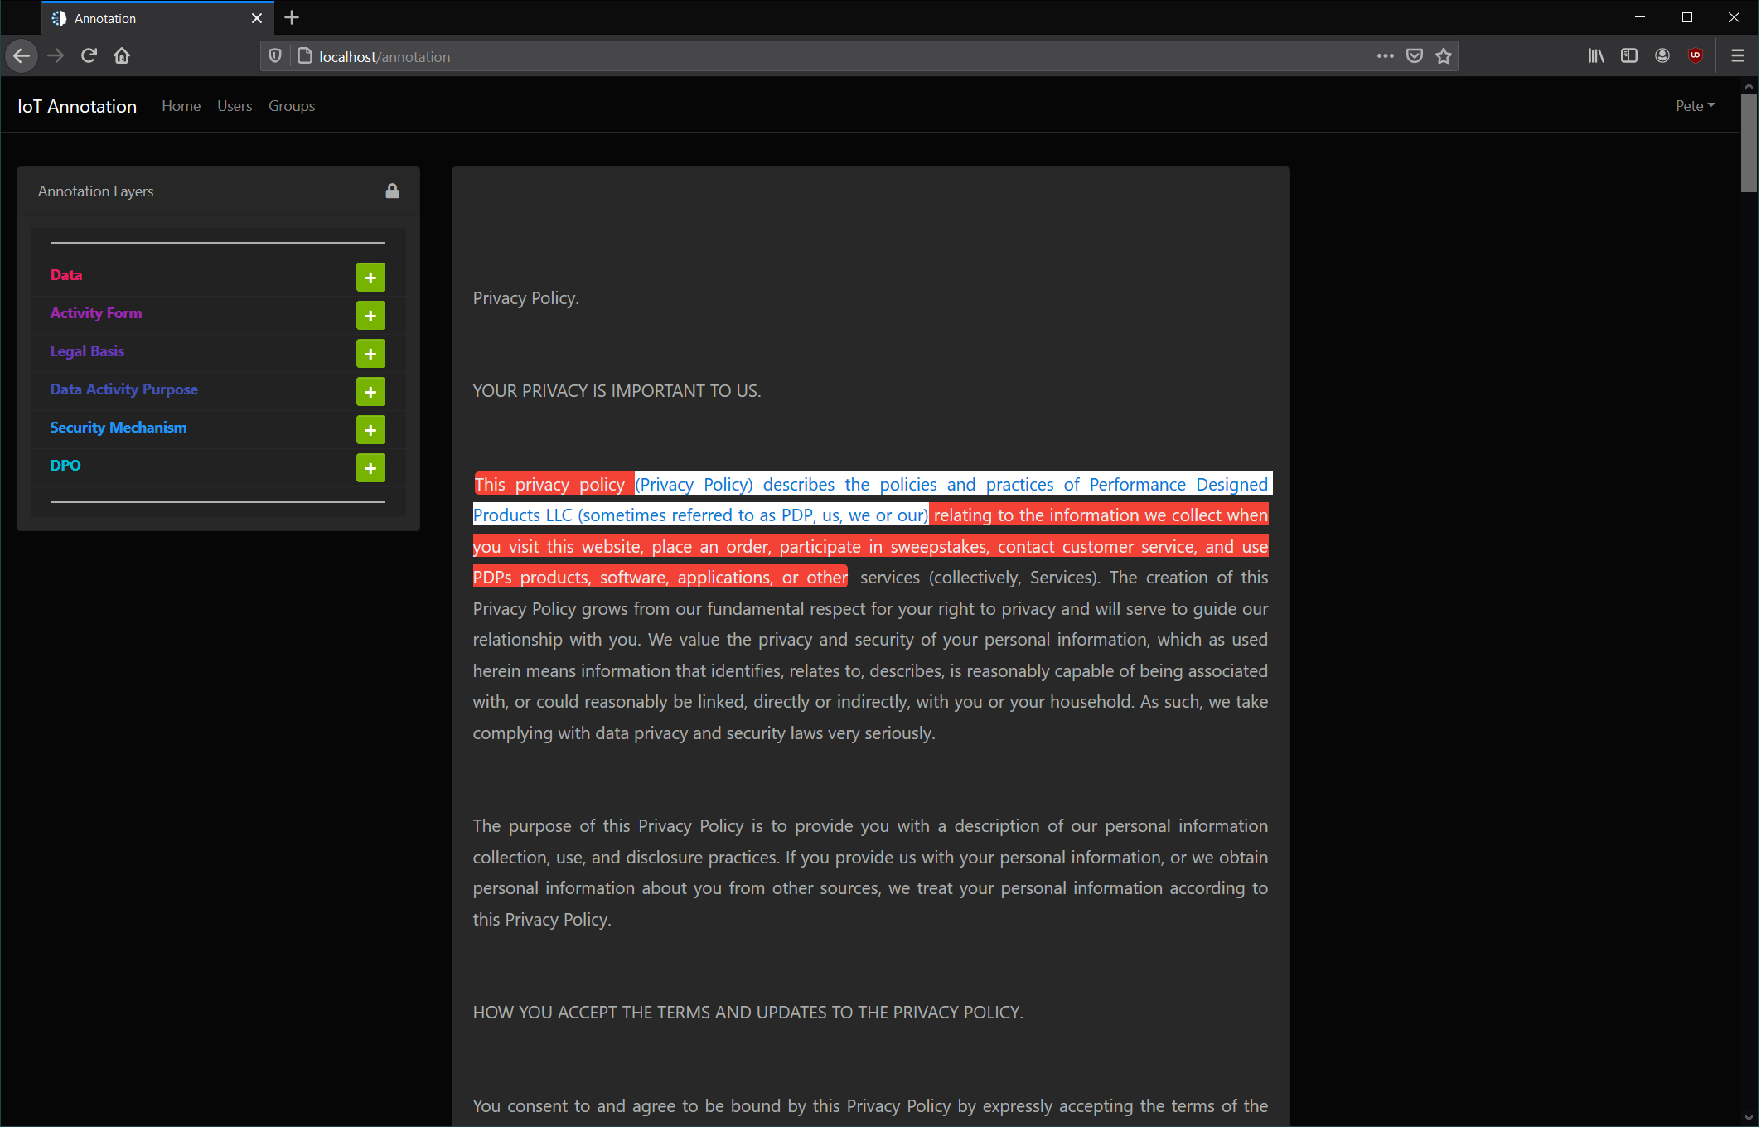
\includegraphics[width=.8\textwidth]{selection2.pdf}}
    \vspace{-\baselineskip}
\end{figure}

На рисунке \ref{fig:result1} представлено состояние страницы разметки после нанесения нескольких неконфликтующих слоев разметки.
\begin{figure}[H]
    \centering
    \ffigbox[\FBwidth]
    {\caption{Нанесение нескольких слоев\label{fig:result1}}}
    {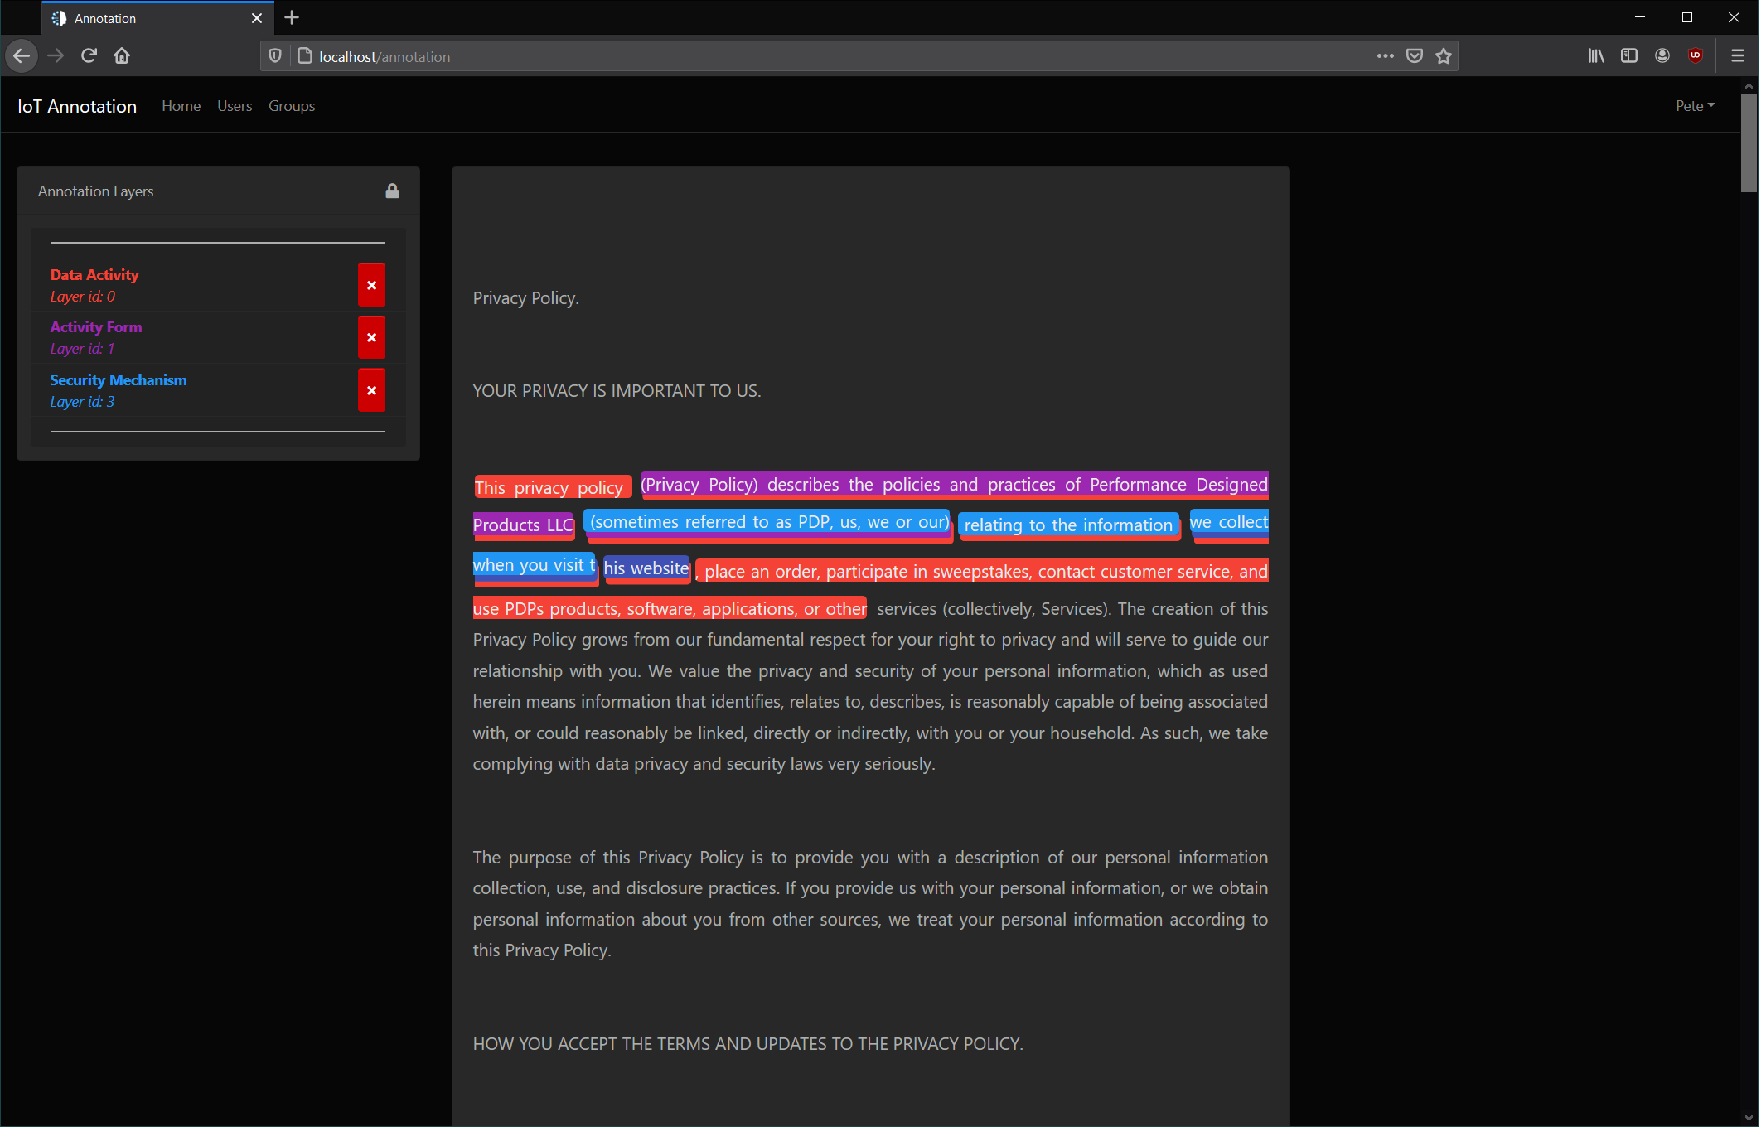
\includegraphics[width=.8\textwidth]{result1.pdf}}
    \vspace{-\baselineskip}
\end{figure}

На рисунке \ref{fig:result2} представлено состояние страницы разметки после удаления одного из слоев разметки. Поверхность аннотирования осуществляет поиск одинаковых по составу слоев разметки и производит их слияние, так что фрагменты с одинаковым набором слоев выглядят целостно.
\begin{figure}[H]
    \centering
    \ffigbox[\FBwidth]
    {\caption{Удаление слоя\label{fig:result2}}}
    {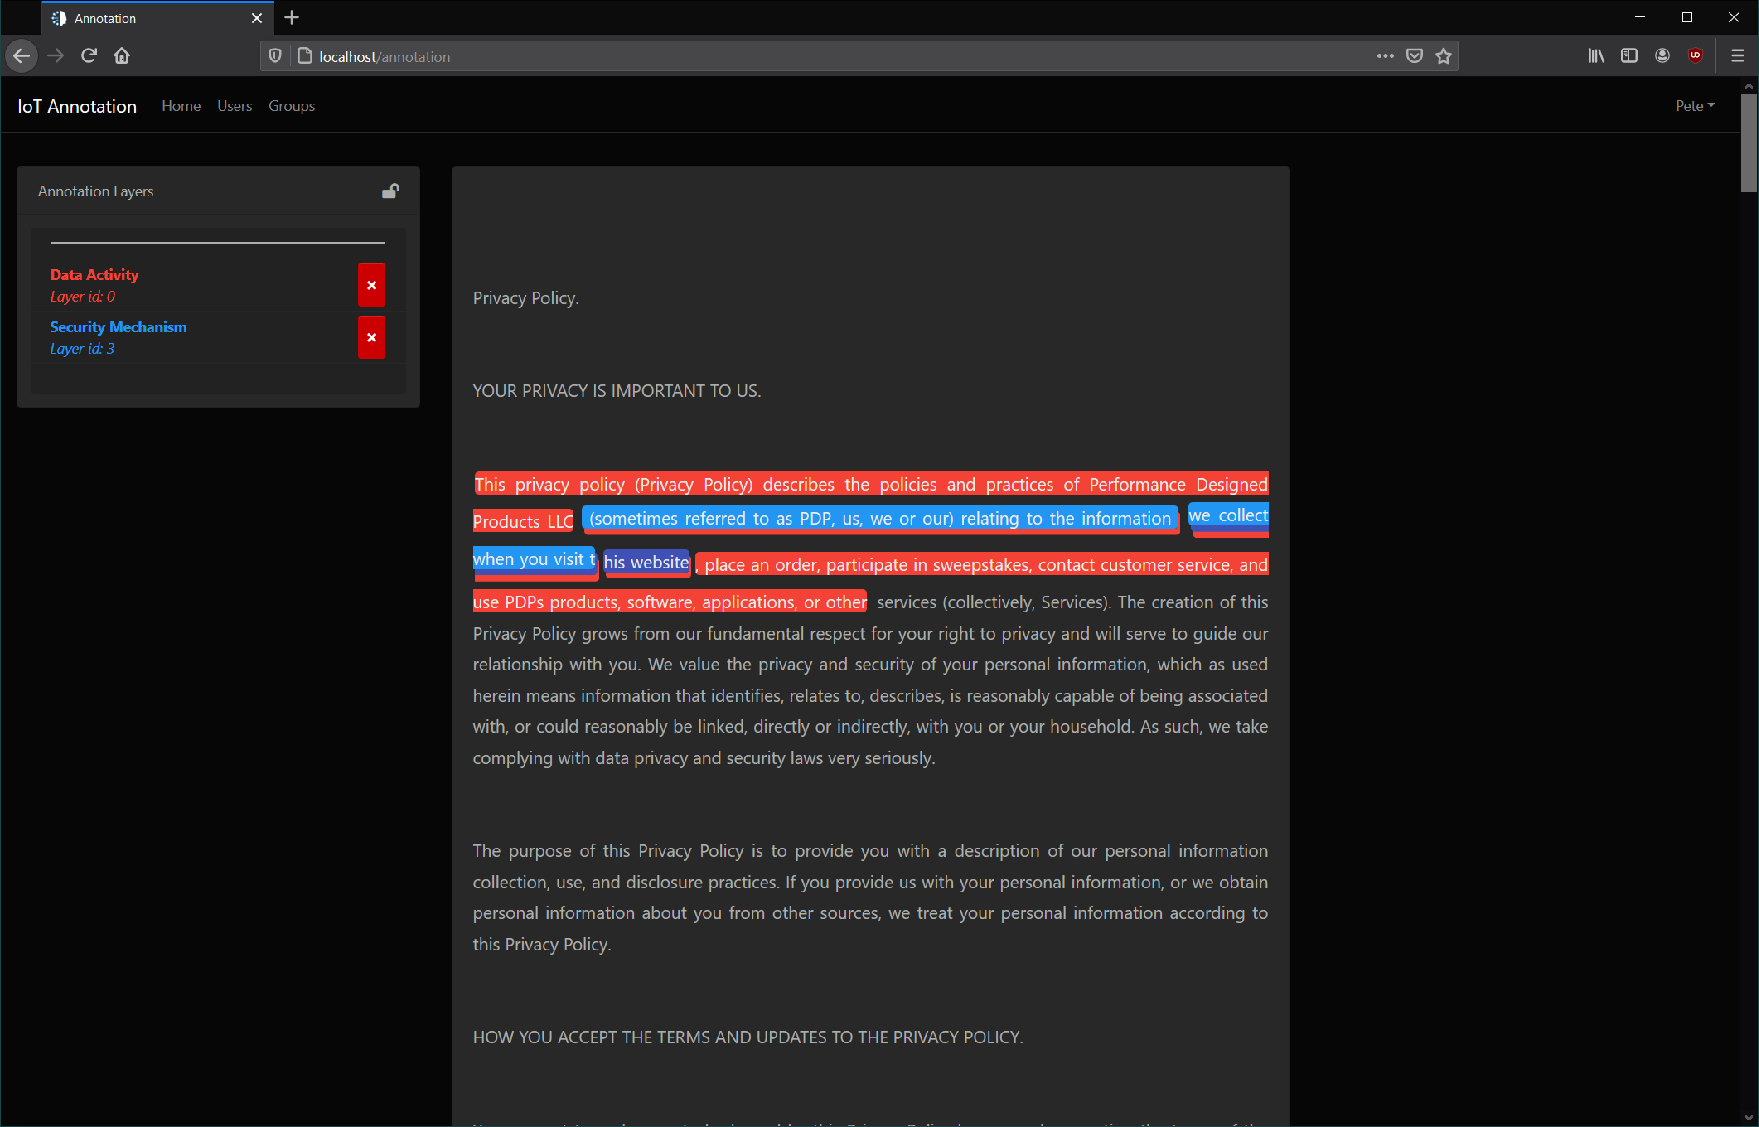
\includegraphics[width=.8\textwidth]{result2.pdf}}
    \vspace{-\baselineskip}
\end{figure}

\subsection{Итоги этапа реализации}

На данном этапе были успешно проведены: моделирование программного решения на разных уровнях с применением универсального языка моделирования UML, реализованы программные компоненты программного пакета, а также выбор программных средств реализации. С помощью разработанного веб-скрейпера с модульной архитектурой был произведен сбор политик безопасности из открытых источников, а именно 592 политики безопасности производителей IoT-устройств. Были подробно рассмотрены статистические и структурные особенности политик безопасности. Полученный датасет имеет ряд преимуществ по сравнению с существующими датасетами, например из работы \cite{MDPI18}, так как он был сформирован в 2021 году, после принятия GDPR в качестве основного международного документа по защите персональных данных. Также датасет является одним из немногих по его тематической ориентации на IoT-устройства. В соответствии с планом по реализации был разработан инструмент разметки текстов политик безопасности для построения обучающей выборки, результат его работы был также представлен.

\newpage
\section{Составление бизнес-плана по коммерциализации результатов научно-исследовательской работы магистра}

\subsection{Описание концепции проекта}
\subsubsection{Название проекта}
В течение работы над научно-исследовательской работой магистра, не было выбрано названия для проекта, исходя из предназначения программного пакета и ориентации на мультиязычную аудиторию стоит выбрать максимально понятное название, возможными вариантами являются:
\begin{enumerate}
    \item Machine Learning Annotation ToolKit
    \item Dataset Mining ToolKit
\end{enumerate}

\subsubsection{Сущность проекта}
В сущности программный пакет представляет из себя набор программ для решения задач по автоматизированному сбору датасетов с их последующей разметкой при помощи инструмента аннотирования, который так же входит в состав данного пакета.

Бизнес-ситуация на данный момент характеризуется следующими особенностями:
\begin{enumerate}
    \item программных пакетов для сбора датасетов практически не найти;
    \item инструменты аннотирования, которые существуют, не обладают необходимым функционалом.
\end{enumerate}

\subsubsection{Реальная бизнес-ситуация, служащая обоснованием проекта}
Задача выпускной квалификационной работы, поставленная в разделе \hyperref[sec:subject_domain]{1}, является актуальной и заслуживает внимания. Данные особенности не позволяют решить задачи, имеющиеся в предметной области выпускной квалификационной работы, на базе существующих решений (образование незанятой рыночной ниши), что автоматически означает необходимость в разработке новых решений. 

\subsubsection{Цели проекта}
Целью проекта является реализация программного пакета для сбора и аннотирования датасетов, соответствующего техническому заданию и требованиям методик, разработанных для решения задач предметной области. Стоит отметить, что проект разрабатывается не сугубо под задачи представленные в разделе \hyperref[sec:subject_domain]{1}, разработанный программный пакет будет способен решать целый класс задач, а именно автоматизированный сбор датасетов из сети Интернет с их последующим аннотированием. 

\subsubsection{Границы проекта}
Проект не включает в себя разработку инструментов для работы с технологиями машинного обучения, на сегодняшний день подобные инструменты представлены на рынке достаточно широко. Также проект не включает в себя проведение аннотирования, так как для этого необходимы эксперты из разных предметных областей (так как инструмент решает целый класс задач сбора и аннотирования датасетов), достаточно компетентные, чтобы создать качественную обучающую выборку для моделей, основанных на технологиях машинного обучения. Обучение моделей, основанных на глубоком обучении, так же не будет производиться, данный шаг будет выполняться отдельно каждым потребителем, который к тому же выберет необходимые для решения своей задачи технологии. Таким образом в проект входит только программное обеспечение -- веб-скрейпер и инструмент аннотирования.

\subsubsection{Допущения}
При нынешнем состоянии предметной области, а именно активном продвижении методик формализации данных, остается нерешенным вопрос формирования обучающих выборок для моделей глубокого обучения. На данный момент исследователи и специалисты в этой области вынуждены под каждую конкретную задачу разрабатывать свой собственный инструмент. Таким образом проект имеет смысл реализовывать при текущем состоянии рынка.

\subsubsection{Заинтересованные стороны проекта}
Потенциальными заинтересованным сторонами проекта являются исследователи, специалисты, энтузиасты, коммерческие организации и некоммерческие организации, работающие в области машинного обучения. Проект создается для удовлетворения их потребностей в инструментах формирования и аннотирования наборов данных для обучения соответствующих моделей. Проект является значимым, потому что он позволит заинтересованным сторонам отойти от разработки инструментов сбора и аннотирования под каждую конкретную задачу, и позволит им, экономя временные, денежные и трудовые ресурсы, заниматься задачами, в которых действительно необходима их компетенция.

\subsubsection{Риски проекта}
К рискам проекта можно отнести некоторую конкуренцию по части инструментов аннотирования, так как имеются некоммерческие разработки под свободными лицензиями. Заинтересованные стороны при ограниченных ресурсах все же могут обращаться к таким разработкам, хотя они не являются продуктами уровня коммерческого производства и зачастую обладают серьезными недостатками. 

\subsubsection{Ориентировочные сроки проекта}
Ориентировочно проект планируется реализовать за 6 календарных месяцев -- это основной цикл разработки. После осуществляется переход на цикл поддержки продукта, предоставлении сервисных услуг, связанных с обслуживанием программного обеспечения и консультациями, планомерная доработка продукта с точки зрения нового функционала.

\subsubsection{Первоначальная организация проекта}
В деятельности организации будут участвовать отделы:
\begin{enumerate}
    \item HR-служба,
    \item отдел системного администрирования,
    \item отдел разработки,
    \item отдел поддержки,
    \item бухгалтерия.
\end{enumerate}

\subsubsection{Ориентировочный бюджет проекта}
Ориентировочный бюджет проекта на первые 6 месяцев активной фазы разработки 6 000 000 рублей, сюда будут входить затраты на заработную плату, страховые отчисления, аренду помещений, электроэнергию и коммунальные услуги.

\subsection{Описание продукции}
Описание продукции приведено в таблице \ref{tab:product_description}.

\begin{ltwrap}{2mm}{1}{\footnotesize}
    \begin{longtable}[H]{|M{.2\x}|M{.8\x}|}
    
        \caption{Описание продукции\label{tab:product_description}} \\\hline
        \multicolumn{1}{|H{.2\x}|}{Ключевые вопросы}
        & \multicolumn{1}{H{.8\x}|}{Комментарии}\\\hline
        \endfirsthead
        \caption*{Продолжение таблицы \ref{tab:product_description}}\\\hline
        \multicolumn{1}{|H{.2\x}|}{Ключевые вопросы}
        & \multicolumn{1}{H{.8\x}|}{Комментарии}\\\hline
        \endhead
        \endfoot
        \endlastfoot

        Наименование продукции
        & Программный комплекс в соответствии с ГОСТ 19.101-77\\
        
        \hline

        Назначение продукта
        & Автоматизированный сбор данных из открытых источников, аннотирование обучающих выборок для моделей машинного обучения\\
        
        \hline

        Основные характеристики продукта
        & Продукт по части автоматизированного сбора данных занимает фактически пустующую нишу, включает важные функции по обходу блокировок и многопроцессному исполнению; по части аннотирования предлагает новый функционал по сравнению с имеющимися конкурентами. Продукция находится на стадии опытно-конструкторских работ\\
        
        \hline

        Потребительские свойства продукции
        & С помощью продукта потребитель затрачивает гораздо меньше времени на разработку инструментов под свои задачи, таким образом расходует больше ресурсов на решаемую им задачу, а не на сбор данных\\
        
        \hline

        Основные конкурентные преимущества продукции
        & Настраиваемая среда сбора данных из открытых источников, конфигурируемое аннотирование с возможностью иерархической пересекающейся разметки. Обход блокировок на сайтах и многопроцессное выполнение\\
        
        \hline

        Основные потребители и направления использования продукции
        & Исследователи, специалисты, энтузиасты, коммерческие организации и некоммерческие организации, работающие в области машинного обучения\\
        
        \hline

        Ассортимент и структура выпуска продукции
        & Предполагается совместная поставка веб-скрейпера и инструмента аннотирования\\
        
        \hline

        Юридическая защищенность продукции
        & Лицензия\\
        
        \hline

        Дополнительные сервисные услуги
        & Поддержка и консультирование пользователей; стоимость данных услуг включается в стоимость подписки\\
        
        \hline
        
    \end{longtable}
\end{ltwrap}

\subsection{Анализ рынка сбыта продукции}
\subsubsection{Положение дел в отрасли}
Отрасль IT и машинного обучения в частности является стремительно развивающейся. Тенденции роста данной отрасли продолжатся и в перспективе, так как машинное обучение позволяет решать множество прикладных задач. В 2020 году объем инвестиций в разработки на основе технологий искусственного интеллекта вырос на 40\%, достигнув \$67,9 млрд. Об этом свидетельствуют данные из отчета AI Index Report 2021 от исследователей Стэнфордского университета. Данная отрасль имеет огромное значение для бизнеса, социального и экономического развития, о чем и свидетельствует статистика по объемам инвестиций. Техническая оснащенность отрасли находится на высочайшем уровне из-за потребности в сложных вычислениях. Однако, помимо коммерческой основы проводятся и некоммерческие исследования, их наличие тоже следует учитывать.

\subsubsection{Характеристика внешней среды проекта}

PEST-анализ приведен в таблице \ref{tab:pest}.

\begin{ltwrap}{2mm}{1}{\footnotesize}
    \begin{longtable}[H]{|C{.2\x}|M{.3\x}|M{.3\x}|C{.2\x}|}
    
        \caption{PEST-анализ\label{tab:pest}} \\\hline
        \multicolumn{1}{|H{.2\x}|}{Область}
        & \multicolumn{1}{H{.3\x}|}{Фактор}
        & \multicolumn{1}{H{.3\x}|}{Состояние}
        & \multicolumn{1}{H{.2\x}|}{Характер влияния}\\\hline
        \endfirsthead
        \caption*{Продолжение таблицы \ref{tab:pest}}\\\hline
        \multicolumn{1}{|H{.2\x}|}{Область}
        & \multicolumn{1}{H{.3\x}|}{Фактор}
        & \multicolumn{1}{H{.3\x}|}{Состояние}
        & \multicolumn{1}{H{.2\x}|}{Характер влияния}\\\hline
        \endhead
        \endfoot
        \endlastfoot
        % 
        % 
        Политическая
        & Санкции
        & Затрудняется взаимодействие с иностранными клиентами и провайдерами услуг
        & Отрицательное\\\hline
        % 
        % 
        Экономическая
        & Рост отрасли
        & Отрасль привлекает большое количество инвестиций
        & Положительное\\\hline
        % 
        % 
        Социальная
        & Рост отрасли
        & Отрасль привлекает большое количество специалистов
        & Положительное\\\hline
        % 
        % 
        & Большое количество кадров на рынке в связи с эпидемиологической обстановкой
        & В связи с эпидемиологической обстановкой большое количество кадров было сокращено, специалисты стали чаще обращать внимание на предложения работы в удаленном формате, появилась возможность искать кадры без географической привязки
        & Положительное\\\cline{2-4}
        % 
        % 
        & Удаленный формат занятости из-за эпидемиологической обстановки
        & Затрудняется коммуникация среди сотрудников, влияние на работоспособность
        & Отрицательное\\\cline{2-4}
        % 
        % 
        & Количество квалифицированных кадров
        & С каждым годом увеличивается количество специалистов в сфере IT, растет количество образовательных мест по IT направлениям
        & Положительное\\\hline
        % 
        % 
        Технологическая
        & Вклад технологии машинного обучения в развитие рынка
        & За последние годы количество инвестиций в технологии машинного обучения стабильно растет, и продолжит свой рост
        & Положительное\\\cline{2-4}
        % 
        % 
        & Широта приложения технологий машинного обучения
        & Обеспечивает востребованность проекта в различных предметных областях, где используется машинное обучение
        & Положительное\\\hline
        % 
        % 
    \end{longtable}
\end{ltwrap}

SWOT-анализ приведен в таблице \ref{tab:swot}.

\begin{ltwrap}{2mm}{1}{\footnotesize}
    \begin{longtable}[H]{|M{.5\x}|M{.5\x}|}
    
        \caption{SWOT-анализ\label{tab:swot}} \\\hline
        \multicolumn{1}{|H{.5\x}|}{Сильные стороны}
        & \multicolumn{1}{H{.5\x}|}{Слабые стороны}\\\hline
        \endfirsthead
        \caption*{Продолжение таблицы \ref{tab:swot}}\\\hline
        \endhead
        \endfoot
        \endlastfoot
        % 
        -- Наличие опции автоматизированного сбора информации,\newline
        -- наличие поддержки пересечения разметки,\newline
        -- наличие поддержки иерархий разметки,\newline
        -- загрузка текстовых корпусов целиком,\newline
        -- поддержка и консультирование клиентов
        & -- Платная основа,\newline
        -- нахождение проекта с стадии опытно-кон\-струк\-тор\-ских работ\\\hline
        % 
        \multicolumn{1}{|H{.5\x}|}{Возможности}
        & \multicolumn{1}{H{.5\x}|}{Угрозы}\\\hline
        -- Наличие опции автоматизированного сбора информации,\newline
        -- обход блокировок и captcha,\newline
        -- наличие поддержки пересечения разметки,\newline
        -- осуществление аннотирования обучающих выборок,\newline
        -- наличие поддержки иерархий разметки,\newline
        -- загрузка текстовых корпусов целиком
        & -- Нежелание потенциального заказчика платить за продукт,\newline
        -- эпидемиологическая обстановка\\\hline
    \end{longtable}
\end{ltwrap}

\subsubsection{Анализ рынка}
Исходя из роста инвестиций в технологии машинного обучения, спрос на продукцию связанную с такими технологиями неуклонно растет. Специалистам в данной области требуются инструменты, сокращающие затраты на разработку вспомогательных программ добычи данных, а также разметки обучающих выборок. Используя готовые решения, специалисты занимаются непосредственно своей основной работой, решают поставленные задачи в кратчайшие сроки, что позволяет производству прогрессировать и расти быстрее. Барьером для удовлетворения потребности можно считать сложность создания гибких инструментов для решения обозначенных ранее задач.

Факторы влияющие на выбор продукта:
\begin{enumerate}
    \item функциональная оснащенность,
    \item стоимость программного продукта,
    \item предоставляемая поддержка и консультирование,
    \item качество программного продукта.
\end{enumerate}

Потенциальные потребители коммерческие и некоммерческие организации (штатные специалисты и исследователи), а также свободные специалисты и исследователи. Специалисты и исследователи постоянно ищут новые подходы к решению задач, и потому следят за профессиональной литературой и публикациями.

\subsubsection{Сегментирование рынка и выбор целевых сегментов}
Далее рассматривается сегментирование рынка. Категории потенциальных пользователей, заинтересованных в программном пакете:
\begin{itemize}
    \item сегментирование по географическому принципу -- приложение будет распространяться не только на территории России, но и других стран, однако стоит отметить, что программный пакет будет переведен только на английский язык;
    \item психографическое сегментирование -- программный пакет может использоваться людьми разных социальных классов, ведущих любой образ жизни;
    \item поло-возрастное сегментирование -- программный пакет может использоваться людьми вне зависимости от их пола и возраста;
    \item демографическое сегментирование рынка -- преимущественно потребителями являются свободные и штатные специалисты в области машинного обучения, обладающие высокими доходами, также потребителями могут быть студенты, для пользования требуется определенный уровень компетенции в области машинного обучения.
\end{itemize}

В связи указанными сегментами планируется использовать модель распространения программного пакета по подписке. Таким образом для охвата всех указанных сегментов будет использована следующая политика распространения:
\begin{itemize}
    \item свободные специалисты оплачивают подписку для физического лица;
    \item студенты, подтвердившие свой статус, получают льготы на оформление подписки для физического лица;
    \item корпоративные клиенты оплачивают подписку для юридических лиц.
\end{itemize}

\subsection{Анализ конкурентов}
Анализ конкурентов приведен в таблице \ref{tab:segments}.

\begin{ltwrap}{2mm}{1}{\footnotesize}
    \begin{longtable}[H]{|C{.2\x}|C{.16\x}|C{.16\x}|C{.16\x}|C{.16\x}|C{.16\x}|}
        \caption{Анализ конкурентов\label{tab:segments}}\\\hline
        \multicolumn{1}{|H{.2\x}|}{Название конкурента/конкурирующего проекта}
        & \multicolumn{1}{H{.16\x}|}{Пересечение разметки}
        & \multicolumn{1}{H{.16\x}|}{Иерархи\-чес\-кая разметка}
        & \multicolumn{1}{H{.16\x}|}{Платная основа}
        & \multicolumn{1}{H{.16\x}|}{Наличие инструмента сбора информации}
        & \multicolumn{1}{H{.16\x}|}{Загрузка текстовых корпусов целиком}\\\hline
        \endfirsthead
        \caption*{Продолжение таблицы \ref{tab:segments}}\\\hline
        \multicolumn{1}{|H{.2\x}|}{Название конкурента/конкурирующего проекта}
        & \multicolumn{1}{H{.16\x}|}{Пересечение разметки}
        & \multicolumn{1}{H{.16\x}|}{Иерархи\-чес\-кая разметка}
        & \multicolumn{1}{H{.16\x}|}{Платная основа}
        & \multicolumn{1}{H{.16\x}|}{Наличие инструмента сбора информации}
        & \multicolumn{1}{H{.16\x}|}{Загрузка текстовых корпусов целиком}\\\hline
        \endhead
        \endfoot
        \endlastfoot
        % 
        Dataset Mining ToolKit
        & +
        & +
        & +
        & +
        & +\\\hline
        % 
        Inception
        & --
        & +
        & --
        & --
        & +\\\hline
        % 
        Doccano
        & --
        & --
        & --
        & --
        & +\\\hline
        % 
        Label Studio
        & --
        & +
        & --
        & --
        & +\\\hline
        
    \end{longtable}
\end{ltwrap}

Конкуренция скорее является неценовой, она основывается на предоставляемом в продукте функционале.

Отсутствие таких функциональных возможностей как пересечение разметки и иерархическая разметка могут пагубно сказаться на качестве и детализации обучающих выборок, а от обучающей выборки напрямую зависит результат работы моделей машинного обучения.

Исходя из представленных данных, можно заключить, что предлагаемая продукция по ряду критериев превосходит конкурентов в своей области. Однако, платная основа распространения может рассматриваться потребителями как недостаток.

\subsection{План маркетинга}

\subsubsection{Товарная политика}
Основными функциональными свойствами продукта являются: осуществление автоматизированного сбора информации, многопроцессный режим, обход блокировок и captcha, наличие поддержки пересечения разметки, осуществление аннотирования обучающих выборок, наличие поддержки иерархий разметки, загрузка текстовых корпусов целиком.

Разрабатываемый программный пакет обладает определенными техническими требованиями:
\begin{itemize}
    \item веб-скрейпер:
    \begin{enumerate}
        \item предустановленный браузер Firefox;
        \item наличие интерпретатора python 3.9;
    \end{enumerate}
    \item инструмент аннотирования:
    \begin{enumerate}
        \item предустановленный веб-сервер;
        \item предустановленная СУБД;
    \end{enumerate}
\end{itemize}

Предлагаемый программный пакет планируется сбывать по разным тарифам (образуя таким образом ассортимент), то есть будет сделан шаг навстречу потребителям, который позволит им оплачивать подписку на продукт в соответствии с их финансовыми возможностями.

Программный продукт будет поставляться в виде цифровой копии, безопасность и защита от хищения будет осуществляться на основе лицензионных ключей.

В качестве дополнительных услуг (включенных в стоимость подписки) будут предоставляться сервисные услуги по настройке и внедрению продукта. Также будут предоставляться услуги по консультированию (также включенных в стоимость подписки).

\subsubsection{Распределительная политика}
География сбыта не привязана к конкретным территориям и регионам, сбыт планируется посредством оформления подписки через интернет сервисы. Таким образом предпочтительным выбран прямой канал сбыта продукции. Так как продукция поставляется в виде электронной копии, доставка не предусматривается.

\subsubsection{Коммуникационная политика}
Целевая аудитория совпадает с целевыми сегментами. Инструментами продвижения продукции могут послужить посты в тематических группах в социальных сетях и на форумах, таким образом планируется охватить аудиторию свободных специалистов и студентов. Также важными являются каналы коммуникации через публикации в журналах, выставки и конференции, таким образом планируется охватить аудиторию занятых специалистов, коммерческие и некоммерческие организации. Также большой успех может принести практикум, размещенный на одном из видеохостингов, который сможет продемонстрировать все возможности программного продукта и в то же время помочь начинающим с его освоением. Указанные каналы продвижения находятся максимально близко к целевой аудитории, поэтому были выбраны именно они. Описание коммуникационной политики приведено в таблице \ref{tab:communications}. Расчет бюджета продвижения и график продвижения представлены в таблицах \ref{tab:promotion} и \ref{tab:promotion_plan} соответственно.

Основная концепция товара -- облегчение труда для специалистов, работающих в сфере машинного обучения, соответственно реклама должна отражать данный факт, так же в рекламе стоит указать о достоинствах продукта по сравнению с конкурентами. 

\begin{ltwrap}{2mm}{1}{\footnotesize}
    \begin{longtable}[H]{|C{.15\x}|M{.35\x}|M{.5\x}|}
        \caption{Концепции и инструменты продвижения\label{tab:communications}}\\\hline
        \multicolumn{1}{|H{.15\x}|}{Инструмент}
        & \multicolumn{1}{H{.35\x}|}{Канал}
        & \multicolumn{1}{H{.5\x}|}{Концепция}\\\hline
        \endfirsthead
        \caption*{Продолжение таблицы \ref{tab:communications}}\\\hline
        \multicolumn{1}{|H{.15\x}|}{Инструмент}
        & \multicolumn{1}{H{.35\x}|}{Канал}
        & \multicolumn{1}{H{.5\x}|}{Концепция}\\\hline
        \endhead
        \endfoot
        \endlastfoot
        % 
        Реклама
        & Реклама в журнале Computer World
        & Описание концепции, почему данный инструмент необходим специалистам области\\\cline{2-3}
        % 
        & Практикум на YouTube
        & В практикуме показываются преимущества программного продукта, знакомство новых пользователей с ним, помощь новичкам в освоении\\\hline
        % 
        Связи с общественностью
        & Обзорные статьи в научном журнале CyberLeninka
        & Описание хода разработки, подходов к решению задач\\\hline
        % 
        Интернет-пред\-ста\-ви\-тель\-ство
        & Веб-страница продукта
        & Одностраничный сайт, для демонстрации возможностей, технических характеристик\\\hline
        % 
    \end{longtable}
\end{ltwrap}

\begin{ltwrap}{2mm}{1}{\footnotesize}
    \begin{longtable}[H]{|C{.16\x}|M{.18\x}|C{.16\x}|M{.18\x}|C{.16\x}|C{.16\x}|}
        \caption{Расчет бюджета продвижения\label{tab:promotion}}\\\hline
        \multicolumn{1}{|H{.16\x}|}{Инструмент}
        & \multicolumn{1}{H{.18\x}|}{Наименование мероприятия}
        & \multicolumn{1}{H{.16\x}|}{Период мероприятия}
        & \multicolumn{1}{H{.18\x}|}{Место размещения}
        & \multicolumn{1}{H{.16\x}|}{Расчет затрат}
        & \multicolumn{1}{H{.16\x}|}{Итого сумма}\\\hline
        \endfirsthead
        \caption*{Продолжение таблицы \ref{tab:promotion}}\\\hline
        \multicolumn{1}{|H{.16\x}|}{Инструмент}
        & \multicolumn{1}{H{.18\x}|}{Наименование мероприятия}
        & \multicolumn{1}{H{.16\x}|}{Период мероприятия}
        & \multicolumn{1}{H{.18\x}|}{Место размещения}
        & \multicolumn{1}{H{.16\x}|}{Расчет затрат}
        & \multicolumn{1}{H{.16\x}|}{Итого сумма}\\\hline
        \endhead
        \endfoot
        \endlastfoot
        % 
        % 
        Реклама
        & Реклама в журнале Computer World
        & 01.09.2021 - 07.09.2021
        & Электронный журнал
        & Размещение рекламы в конце журнала
        & 285 560 руб.\\\cline{2-6}
        % https://www.prosmi.ru/catalog/37
        % 
        % 
        & Практикум на YouTube
        & 08.09.2021 - 15.09.2021
        & Видеохостинг YouTube
        & Съемка (50000 руб.) + монтаж (20000 руб.)
        & 70 000 руб.\\\hline
        % https://www.prosmi.ru/catalog/37
        % 
        % 
        Связи с обществен­ностью
        & Подготовка публикации в CyberLeninka
        & 01.01.2022 - 07.01.2022
        & Электронный научный журнал
        & Услуги редактора
        & 20 000 руб.\\\cline{2-6}
        % 
        % 
        & Подготовка публикации в CyberLeninka
        & 01.01.2023 - 07.01.2023
        & Электронный научный журнал
        & Услуги редактора
        & 20 000 руб.\\\hline
        % 
        % 
        Интернет-­пред\-ста\-ви\-­тель\-ство
        & Одностраничное веб-приложение
        & 01.09.2021 - 24.09.2021
        & сеть Интернет
        & Разработка веб-приложения
        & 149 800 руб.\\\hline
        % https://expodev.org/%D0%B7%D0%B0%D0%BA%D0%B0%D0%B7%D0%B0%D1%82%D1%8C-single-page-application/
        % 
        \multicolumn{5}{|C{.84\x}|}{Итого на продвижение} 
        & 545 360 руб.\\\hline
    \end{longtable}
\end{ltwrap}

\begin{ltwrap}{2mm}{1}{\footnotesize}
    \begin{longtable}[H]{|C{.2\x}|C{.066\x}|C{.066\x}|C{.066\x}|C{.066\x}|C{.066\x}|C{.066\x}|C{.066\x}|C{.066\x}|C{.066\x}|C{.066\x}|C{.066\x}|C{.066\x}|}
        \caption{График продвижения\label{tab:promotion_plan}}\\\hline
        \multicolumn{1}{|H{.2\x}|}{\multirow{2}{*}{Мероприятие}} 
        & \multicolumn{12}{H{.8\x}|}{Кварталы}\\\cline{2-13}
        & \multicolumn{1}{H{.066\x}|}{I}
        & \multicolumn{1}{H{.066\x}|}{II}
        & \multicolumn{1}{H{.066\x}|}{III}
        & \multicolumn{1}{H{.066\x}|}{IV}
        & \multicolumn{1}{H{.066\x}|}{I}
        & \multicolumn{1}{H{.066\x}|}{II}
        & \multicolumn{1}{H{.066\x}|}{III}
        & \multicolumn{1}{H{.066\x}|}{IV}
        & \multicolumn{1}{H{.066\x}|}{I}
        & \multicolumn{1}{H{.066\x}|}{II}
        & \multicolumn{1}{H{.066\x}|}{III}
        & \multicolumn{1}{H{.066\x}|}{IV}\\\hline
        \endfirsthead
        \caption*{Продолжение таблицы \ref{tab:promotion_plan}}\\\hline
        \multicolumn{1}{|H{.2\x}|}{\multirow{2}{*}{Мероприятие}} 
        & \multicolumn{12}{H{.8\x}|}{Кварталы}\\\cline{2-13}
        & \multicolumn{1}{H{.066\x}|}{I}
        & \multicolumn{1}{H{.066\x}|}{II}
        & \multicolumn{1}{H{.066\x}|}{III}
        & \multicolumn{1}{H{.066\x}|}{IV}
        & \multicolumn{1}{H{.066\x}|}{I}
        & \multicolumn{1}{H{.066\x}|}{II}
        & \multicolumn{1}{H{.066\x}|}{III}
        & \multicolumn{1}{H{.066\x}|}{IV}
        & \multicolumn{1}{H{.066\x}|}{I}
        & \multicolumn{1}{H{.066\x}|}{II}
        & \multicolumn{1}{H{.066\x}|}{III}
        & \multicolumn{1}{H{.066\x}|}{IV}\\\hline
        \endhead
        \endfoot
        \endlastfoot
        % 
        Реклама в журнале Computer World
        & 
        & 
        & 
        & $\times$
        & 
        &
        & 
        & 
        & 
        &
        & 
        & \\\hline
        % 
        Практикум на YouTube
        & 
        & 
        & $\times$
        & $\times$
        & $\times$
        & $\times$
        & $\times$
        & $\times$
        & $\times$
        & $\times$
        & $\times$
        & $\times$\\\hline
        % 
        Подготовка публикации в CyberLeninka
        & 
        & 
        & 
        &
        & $\times$
        & 
        & 
        &
        & $\times$
        &
        & 
        & \\\hline
        % 
        Одностраничное веб-­приложение
        & 
        & 
        & $\times$
        & $\times$
        & $\times$
        & $\times$
        & $\times$
        & $\times$
        & $\times$
        & $\times$
        & $\times$
        & $\times$\\\hline
        % 
    \end{longtable}
\end{ltwrap}


\subsubsection{Ценовая политика}
Стратегия ценообразования учитывает разные сегменты рынка. Так разным потребителям будут поставляться одни и те же продукты, но по разным ценам. Цены для организаций будут значительно выше, чем для свободных специалистов исследователей и студентов. Студенты получают льготы -- снижение стоимости подписки на программный продукт. Подписка на продукт оформляется на 3 месяца.

Цены на продукцию высчитываются из срока окупаемости, так как продукт не требует производства для продажи, он разрабатывается один раз и затем сбывается потребителям в виде копий.

\subsubsection{План продаж}

План продаж рассчитанный на 3 года представлен в таблицах \ref{tab:sells_plan}, \ref{tab:sells_plan2} и \ref{tab:sells_plan3}. Здесь <<п. физ.>> -- подписка для физических лиц, <<п. юр.>> -- подписка для юридических лиц, <<п. ст.>> -- подписка для студентов. В начале ожидается быстрый рост продаж в связи с продвижением продукта, соответственно в кварталах, где проводилось продвижение ожидается рост сбыта. При этом определенное количество потребителей будут отказываться от продукта. Те потребители, которые будут довольны продуктом, будут продлевать подписку. Подобное продвижение будет сделано и спустя год после выхода продукта на рынок, чтобы поддерживать количество потребителей. Планомерная доработка продукта отделом разработки будет так же удерживать определенное количество клиентов. В первом и втором кварталах каждого года предположительно будет происходить рост сбыта льготных подписок студентам, в связи с выполнением курсовых и дипломных работ.

\begin{ltwrap}{2mm}{1}{\footnotesize}
    \begin{longtable}[H]{|C{.14\x}|C{.18\x}|C{.18\x}|C{.18\x}|C{.18\x}|C{.14\x}|}
        \caption{План продаж, год 1\label{tab:sells_plan}}\\\hline
        \multicolumn{1}{|H{.14\x}|}{\multirow{2}{*}{Показатели}} 
        & \multicolumn{4}{H{.72\x}|}{Кварталы}
        & \multicolumn{1}{H{.14\x}|}{\multirow{2}{*}{Всего}}\\\cline{2-5}
        & \multicolumn{1}{H{.18\x}|}{I}
        & \multicolumn{1}{H{.18\x}|}{II}
        & \multicolumn{1}{H{.18\x}|}{III}
        & \multicolumn{1}{H{.18\x}|}{IV}
        & \\\hline
        \endfirsthead
        \caption*{Продолжение таблицы \ref{tab:sells_plan}}\\\hline
        \multicolumn{1}{|H{.14\x}|}{\multirow{2}{*}{Показатели}} 
        & \multicolumn{4}{H{.72\x}|}{Кварталы}
        & \multicolumn{1}{H{.14\x}|}{\multirow{2}{*}{Всего}}\\\cline{2-5}
        & \multicolumn{1}{H{.18\x}|}{I}
        & \multicolumn{1}{H{.18\x}|}{II}
        & \multicolumn{1}{H{.18\x}|}{III}
        & \multicolumn{1}{H{.18\x}|}{IV}
        & \\\hline
        \endhead
        \endfoot
        \endlastfoot
        % 
        % 1 250, 625, 62 500
        Ожидаемый объем продаж, ед.
        & --
        & --
        & 2000 п. физ. 50 п. юр. 1900 п. ст.
        & 2500 п. физ. 75 п. юр. 1200 п. ст.
        & 5500 п. физ. 125 п. юр. 3100 п. ст.\\\hline
        % 
        % 
        Цена с НДС, тыс. руб.
        & --
        & --
        & 1,250 п. физ. 62,5 п. юр. 0,625 п. ст.
        & 1,250 п. физ. 62,5 п. юр. 0,625 п. ст.
        & 1,250 п. физ. 62,5 п. юр. 0,625 п. ст.\\\hline
        % 
        % 
        Выручка с НДС, тыс. руб.
        & --
        & --
        & 6 813
        & 8 563
        & 15 375\\\hline
        % 
        % 
        Сумма НДС, тыс. руб.
        & --
        & --
        & 1 363
        & 1 713
        & 3 075\\\hline
        % 
        % 
        Нетто-выручка (без НДС), тыс. руб.
        & --
        & --
        & 5 450
        & 6 850
        & 12 300\\\hline
        % 
        % 
    \end{longtable}
\end{ltwrap}

\begin{ltwrap}{2mm}{1}{\footnotesize}
    \begin{longtable}[H]{|C{.14\x}|C{.18\x}|C{.18\x}|C{.18\x}|C{.18\x}|C{.14\x}|}
        \caption{План продаж, год 2\label{tab:sells_plan2}}\\\hline
        \multicolumn{1}{|H{.14\x}|}{\multirow{2}{*}{Показатели}} 
        & \multicolumn{4}{H{.72\x}|}{Кварталы}
        & \multicolumn{1}{H{.14\x}|}{\multirow{2}{*}{Всего}}\\\cline{2-5}
        & \multicolumn{1}{H{.18\x}|}{I}
        & \multicolumn{1}{H{.18\x}|}{II}
        & \multicolumn{1}{H{.18\x}|}{III}
        & \multicolumn{1}{H{.18\x}|}{IV}
        & \\\hline
        \endfirsthead
        \caption*{Продолжение таблицы \ref{tab:sells_plan2}}\\\hline
        \multicolumn{1}{|H{.14\x}|}{\multirow{2}{*}{Показатели}} 
        & \multicolumn{4}{H{.72\x}|}{Кварталы}
        & \multicolumn{1}{H{.14\x}|}{\multirow{2}{*}{Всего}}\\\cline{2-5}
        & \multicolumn{1}{H{.18\x}|}{I}
        & \multicolumn{1}{H{.18\x}|}{II}
        & \multicolumn{1}{H{.18\x}|}{III}
        & \multicolumn{1}{H{.18\x}|}{IV}
        & \\\hline
        \endhead
        \endfoot
        \endlastfoot
        % 
        Ожидаемый объем продаж, ед.
        & 1300 п. физ. 55 п. юр. 1500 п. ст.
        & 1400 п. физ. 60 п. юр. 1100 п. ст.
        & 1500 п. физ. 50 п. юр. 600 п. ст.
        & 1200 п. физ. 55 п. юр. 400 п. ст.
        & 5400 п. физ. 220 п. юр. 3600 п. ст.\\\hline
        % 
        % 
        Цена с НДС, тыс. руб.
        & 1,250 п. физ. 62,5 п. юр. 0,625 п. ст.
        & 1,250 п. физ. 62,5 п. юр. 0,625 п. ст.
        & 1,250 п. физ. 62,5 п. юр. 0,625 п. ст.
        & 1,250 п. физ. 62,5 п. юр. 0,625 п. ст.
        & 1,250 п. физ. 62,5 п. юр. 0,625 п. ст.\\\hline
        % 
        % 
        Выручка с НДС, тыс. руб.
        & 6 000
        & 6 188
        & 5 375
        & 5 188
        & 22 750\\\hline
        % 
        % 
        Сумма НДС, тыс. руб.
        & 1 200
        & 1 238
        & 1 075
        & 1 038
        & 4 550\\\hline
        % 
        % 
        Нетто-выручка (без НДС), тыс. руб.
        & 4 800
        & 4 950
        & 4 300
        & 4 150
        & 18 200\\\hline
        % 
        % 
    \end{longtable}
\end{ltwrap}

\begin{ltwrap}{2mm}{1}{\footnotesize}
    \begin{longtable}[H]{|C{.14\x}|C{.18\x}|C{.18\x}|C{.18\x}|C{.18\x}|C{.14\x}|}
        \caption{План продаж, год 3\label{tab:sells_plan3}}\\\hline
        \multicolumn{1}{|H{.14\x}|}{\multirow{2}{*}{Показатели}} 
        & \multicolumn{4}{H{.72\x}|}{Кварталы}
        & \multicolumn{1}{H{.14\x}|}{\multirow{2}{*}{Всего}}\\\cline{2-5}
        & \multicolumn{1}{H{.18\x}|}{I}
        & \multicolumn{1}{H{.18\x}|}{II}
        & \multicolumn{1}{H{.18\x}|}{III}
        & \multicolumn{1}{H{.18\x}|}{IV}
        & \\\hline
        \endfirsthead
        \caption*{Продолжение таблицы \ref{tab:sells_plan3}}\\\hline
        \multicolumn{1}{|H{.14\x}|}{\multirow{2}{*}{Показатели}} 
        & \multicolumn{4}{H{.72\x}|}{Кварталы}
        & \multicolumn{1}{H{.14\x}|}{\multirow{2}{*}{Всего}}\\\cline{2-5}
        & \multicolumn{1}{H{.18\x}|}{I}
        & \multicolumn{1}{H{.18\x}|}{II}
        & \multicolumn{1}{H{.18\x}|}{III}
        & \multicolumn{1}{H{.18\x}|}{IV}
        & \\\hline
        \endhead
        \endfoot
        \endlastfoot
        % 
        Ожидаемый объем продаж, ед.
        & 1400 п. физ. 60 п. юр. 1400 п. ст.
        & 1300 п. физ. 65 п. юр. 1200 п. ст.
        & 1400 п. физ. 55 п. юр. 500 п. ст.
        & 1200 п. физ. 60 п. юр. 500 п. ст.
        & 5300 п. физ. 240 п. юр. 3600 п. ст.\\\hline
        % 
        % 
        Цена с НДС, тыс. руб.
        & 1,250 п. физ. 62,5 п. юр. 0,625 п. ст.
        & 1,250 п. физ. 62,5 п. юр. 0,625 п. ст.
        & 1,250 п. физ. 62,5 п. юр. 0,625 п. ст.
        & 1,250 п. физ. 62,5 п. юр. 0,625 п. ст.
        & 1,250 п. физ. 62,5 п. юр. 0,625 п. ст.\\\hline
        % 
        % 
        Выручка с НДС, тыс. руб.
        & 6 375
        & 6 438
        & 5 500
        & 5 563
        & 23 875\\\hline
        % 
        % 
        Сумма НДС, тыс. руб.
        & 1 275
        & 1 288
        & 1 100
        & 1 113
        & 4 775\\\hline
        % 
        % 
        Нетто-выручка (без НДС), тыс. руб.
        & 5 100
        & 5 150
        & 4 400
        & 4 450
        & 19 100\\\hline
        % 
        % 
    \end{longtable}
\end{ltwrap}


\subsection{План производства}

% Офис 58,6 м² за 46 880 руб./мес. https://spb.cian.ru/rent/commercial/256033112/

\subsubsection{Производственная база}
Деятельность будет осуществляться на вновь создаваемом предприятии. Планируется аренда офисного помещения. Для размещения 6 сотрудников, планируется арендовать помещение площадью 60 кв.м. Исходя из стоимости аренды, был выбран офис в Кировском районе г. Санкт-Петербурга по адресу Промышленная ул., 14а с арендной платой 46 880 руб. в месяц. Ремонт офисного помещения не планируется, так как оно находится в удовлетворительном состоянии. 

Потребность в офисной мебели представлена в таблице \ref{tab:furniture}.

\begin{ltwrap}{2mm}{1}{\footnotesize}
    \begin{longtable}[H]{|C{.05\x}|M{.5\x}|C{.15\x}|C{.15\x}|C{.15\x}|}
        \caption{Потребность в офисной мебели\label{tab:furniture}}\\\hline
        \multicolumn{1}{|H{.05\x}|}{№} 
        & \multicolumn{1}{H{.5\x}|}{Наименование}
        & \multicolumn{1}{H{.15\x}|}{Стоимость с НДС, руб.}
        & \multicolumn{1}{H{.15\x}|}{Количество}
        & \multicolumn{1}{H{.15\x}|}{Сумма с НДС, руб.}\\\hline
        \endfirsthead
        \caption*{Продолжение таблицы \ref{tab:furniture}}\\\hline
        \multicolumn{1}{|H{.05\x}|}{№} 
        & \multicolumn{1}{H{.5\x}|}{Наименование}
        & \multicolumn{1}{H{.15\x}|}{Стоимость с НДС, руб.}
        & \multicolumn{1}{H{.15\x}|}{Количество}
        & \multicolumn{1}{H{.15\x}|}{Сумма с НДС, руб.}\\\hline
        \endhead
        \endfoot
        \endlastfoot
        % 
        1
        & Стол рабочий <<Матрица>> венге
        & 2 554
        & 6
        & 15 324\\\hline
        % 
        2
        & Кресло офисное Бюрократ T-898/3С1GR серое
        & 5 099
        & 6
        & 30 594\\\hline
        % 
        3
        & Шкаф архивный ПАКС-металл ШАМ-11
        & 9 559
        & 2
        & 19 118\\\hline
        % 
        4
        & Доска комбинированная магнитно-маркерно-меловая BRAUBERG Premium
        & 11 521
        & 1
        & 11 521\\\hline
        % 
        \multicolumn{4}{|C{.7625\x}|}{Всего}
        & 76 557\\\hline
        % 
    \end{longtable}
\end{ltwrap}

Потребность в производственном оборудовании представлена в таблице \ref{tab:accessories}.

\begin{ltwrap}{2mm}{1}{\footnotesize}
    \begin{longtable}[H]{|C{.05\x}|M{.5\x}|C{.15\x}|C{.15\x}|C{.15\x}|}
        \caption{Потребность в производственном оборудовании\label{tab:accessories}}\\\hline
        \multicolumn{1}{|H{.05\x}|}{№} 
        & \multicolumn{1}{H{.5\x}|}{Наименование}
        & \multicolumn{1}{H{.15\x}|}{Стоимость с НДС, руб.}
        & \multicolumn{1}{H{.15\x}|}{Количество}
        & \multicolumn{1}{H{.15\x}|}{Сумма с НДС, руб.}\\\hline
        \endfirsthead
        \caption*{Продолжение таблицы \ref{tab:accessories}}\\\hline
        \multicolumn{1}{|H{.05\x}|}{№} 
        & \multicolumn{1}{H{.5\x}|}{Наименование}
        & \multicolumn{1}{H{.15\x}|}{Стоимость с НДС, руб.}
        & \multicolumn{1}{H{.15\x}|}{Количество}
        & \multicolumn{1}{H{.15\x}|}{Сумма с НДС, руб.}\\\hline
        \endhead
        \endfoot
        \endlastfoot
        % 
        1
        & Системный блок Atlas H286
        & 36 999
        & 6
        & 221 994\\\hline
        %
        % 
        2
        & Монитор Samsung S24F354FHI
        & 8 899
        & 8
        & 71 192\\\hline
        % 
        % 
        3
        & Компактная мышь беспроводная Microsoft Bluetooth Mobile 3600 черная
        & 1 499
        & 6
        & 8 994\\\hline
        % 
        % 
        4
        & Клавиатура Microsoft Bluetooth
        & 3 050
        & 6
        & 18 300\\\hline
        % 
        % 
        5
        & Веб-камера Canyon CNE-CWC1
        & 1 250
        & 6
        & 7 500\\\hline
        % 
        % 
        6
        & Bluetooth гарнитура DEXP BT-212 черная
        & 1 049
        & 6
        & 6 294\\\hline
        % 
        % 
        7
        & МФУ лазерное HP LaserJet Pro MFP M28a
        & 9 999
        & 1
        & 9 999\\\hline
        % 
        % 
        \multicolumn{4}{|C{.7625\x}|}{Всего}
        & 344 273\\\hline
        % 
    \end{longtable}
\end{ltwrap}

\subsubsection{Потребность в производственном персонале}

Потребность в персонале представлена в таблице \ref{tab:workers}.

\begin{ltwrap}{2mm}{1}{\footnotesize}
    \begin{longtable}[H]{|C{.05\x}|M{.2\x}|C{.2\x}|C{.1375\x}|C{.1375\x}|C{.1375\x}|C{.1375\x}|}
        \caption{Потребность в производственном персонале\label{tab:workers}}\\\hline
        \multicolumn{1}{|H{.05\x}|}{№} 
        & \multicolumn{1}{H{.2\x}|}{Специальность}
        & \multicolumn{1}{H{.2\x}|}{Вид}
        & \multicolumn{1}{H{.1375\x}|}{Чис\-лен\-ность, чел.}
        & \multicolumn{1}{H{.1375\x}|}{Рабочих часов в неделю}
        & \multicolumn{1}{H{.1375\x}|}{Заработная плата в месяц, руб.}
        & \multicolumn{1}{H{.1375\x}|}{Заработная плата за квартал, руб.}\\\hline
        \endfirsthead
        \caption*{Продолжение таблицы \ref{tab:workers}}\\\hline
        \multicolumn{1}{|H{.05\x}|}{№} 
        & \multicolumn{1}{H{.2\x}|}{Специальность}
        & \multicolumn{1}{H{.2\x}|}{Вид}
        & \multicolumn{1}{H{.1375\x}|}{Чис\-лен\-ность, чел.}
        & \multicolumn{1}{H{.1375\x}|}{Рабочих часов в неделю}
        & \multicolumn{1}{H{.1375\x}|}{Заработная плата в месяц, руб.}
        & \multicolumn{1}{H{.1375\x}|}{Заработная плата за квартал, руб.}\\\hline
        \endhead
        \endfoot
        \endlastfoot
        % 
        % 
        1
        & Системный администратор
        & Управляющий
        & 1
        & 40
        & 70 000
        & 210 000\\\hline
        % 
        % 
        2
        & Фронтенд-Разработчик
        & Неуправляющий
        & 1
        & 40
        & 80 000
        & 240 000\\\hline
        % 
        % 
        3
        & Бэкенд-разработчик
        & Неуправляющий
        & 1
        & 40
        & 110 000
        & 330 000\\\hline
        % 
        % 
        4
        & Бухгалтер
        & Управляющий
        & 1
        & 40
        & 50 000
        & 150 000\\\hline
        % 
        % 
        5
        & HR-специалист
        & Управляющий
        & 1
        & 40
        & 40 000
        & 120 000\\\hline
        % 
        % 
        6
        & Специалист по работе с клиентами
        & Управляющий
        & 1
        & 40
        & 50 000
        & 150 000\\\hline
        % 
        % 
    \end{longtable}
\end{ltwrap}

\subsubsection{Расчет общепроизводственных затрат}

Расчет общепроизводственных затрат, исходя из затрат на коммунальные услуги 30 000 руб. плюс 6 000 руб. НДС, и заработной платы неуправляющего персонала 190 000 руб. составит 226 000 руб. Таким образом общепроизводственных затраты в месяц составляют 226 000 руб. в месяц или 678 000 руб. за квартал.

\subsubsection{Расчет общехозяйственных, управленческих и коммерческих расходов}

Амортизация оборудования (линейная), учитывая срок полезного использования компьютера и компьютерной периферии в 3 года (36 месяцев), стоимость оборудования 344 273 руб., будет составлять 2,8\% в месяц, то есть 9 639,64 руб. в месяц (28 918,92 руб. за квартал), а в последний месяц с учетом остатка 2\%, то есть 6 885,46 руб. (26 164,74 руб. за квартал).

Расчет общехозяйственных, управленческих и коммерческих расходов приведен в таблице \ref{tab:losses}, в скобках указана сумма за последний месяц с учетом амортизации.

\begin{ltwrap}{2mm}{1}{\footnotesize}
    \begin{longtable}[H]{|C{.05\x}|M{.55\x}|C{.2\x}|C{.2\x}|}
        \caption{Расчет общехозяйственных, управленческих и коммерческих расходов\label{tab:losses}}\\\hline
        \multicolumn{1}{|H{.05\x}|}{№} 
        & \multicolumn{1}{H{.55\x}|}{Вид расходов}
        & \multicolumn{1}{H{.2\x}|}{В месяц, руб.}
        & \multicolumn{1}{H{.2\x}|}{За квартал, руб.}\\\hline
        \endfirsthead
        \caption*{Продолжение таблицы \ref{tab:losses}}\\\hline
        \multicolumn{1}{|H{.05\x}|}{№} 
        & \multicolumn{1}{H{.55\x}|}{Вид расходов}
        & \multicolumn{1}{H{.2\x}|}{В месяц, руб.}
        & \multicolumn{1}{H{.2\x}|}{За квартал, руб.}\\\hline
        \endhead
        \endfoot
        \endlastfoot
        % 
        % 
        1
        & Амортизация оборудования
        & 9 639,64 (6 885,46)
        & 28 918,92 (26 164,74)\\\hline
        % 
        % 
        2
        & Заработная плата управляющего персонала
        & 210 000
        & 630 000\\\hline
        % 
        % 
        3
        & Отчисления на социальные нужды административно управленческого персонала 30\% 
        & 63 000
        & 189 000\\\hline
        % 
        % 
        4
        & Отчисления на социальные нужды административно неуправленческого персонала 30\% 
        & 57 000
        & 171 000\\\hline
        % 
        % 
        5
        & Аренды производственного помещения
        & 46 880
        & 140 640\\\hline
        % 
        % 
        6
        & Услуги связи
        & 10 000
        & 30 000\\\hline
        % 
        % 
        7
        & Канцелярские товары
        & 3 000
        & 9 000\\\hline
        % 
        % 
        8
        & Выплата по кредиту
        & 180 123
        & 540 369\\\hline
        % 
        % 
        \multicolumn{2}{|C{.6\x}|}{Всего}
        & 579 642,64 (576 888,46)
        & 1 738 927,92 (1 736 173,74)\\\hline
        %
        % 
    \end{longtable}
\end{ltwrap}

Учитываются также коммерческие расходы по рекламе и продвижению в соответствии с таблицами \ref{tab:promotion} и \ref{tab:promotion_plan}. 

\subsubsection{Расчет инвестиционных расходов}

Расчет инвестиционных расходов приведен в таблице \ref{tab:investments}.

\begin{ltwrap}{2mm}{1}{\footnotesize}
    \begin{longtable}[H]{|C{.05\x}|M{.75\x}|C{.2\x}|}
        \caption{Расчет инвестиционных расходов\label{tab:investments}}\\\hline
        \multicolumn{1}{|H{.05\x}|}{№} 
        & \multicolumn{1}{H{.75\x}|}{Наименование сумма}
        & \multicolumn{1}{H{.2\x}|}{Сумма, руб.}\\\hline
        \endfirsthead
        \caption*{Продолжение таблицы \ref{tab:investments}}\\\hline
        \multicolumn{1}{|H{.05\x}|}{№} 
        & \multicolumn{1}{H{.75\x}|}{Наименование сумма}
        & \multicolumn{1}{H{.2\x}|}{Сумма, руб.}\\\hline
        \endhead
        \endfoot
        \endlastfoot
        % 
        % 
        1
        & Закупка офисного оборудования
        & 344 273\\\hline
        % 
        % 
        2
        & Закупка офисной мебели
        & 76 557\\\hline
        % 
        % 
        3
        & Регистрация предприятия, подготовка производства
        & 6 700\\\hline
        % 
        % 
        \multicolumn{2}{|C{.8\x}|}{Всего}
        & 432 530\\\hline
        % 
        % 
    \end{longtable}
\end{ltwrap}

\subsubsection{Расчет затрат на разработку продукта}

Расчет затрат на разработку продукта приведен в таблице \ref{tab:selfcost}. Он произведен с учетом первых 2 кварталов разработки, до момента выпуска продукта на рынок.

\begin{ltwrap}{2mm}{1}{\footnotesize}
    \begin{longtable}[H]{|C{.05\x}|M{.75\x}|C{.2\x}|}
        \caption{Расчет затрат на разработку продукта\label{tab:selfcost}}\\\hline
        \multicolumn{1}{|H{.05\x}|}{№} 
        & \multicolumn{1}{H{.75\x}|}{Наименование сумма}
        & \multicolumn{1}{H{.2\x}|}{Сумма, руб.}\\\hline
        \endfirsthead
        \caption*{Продолжение таблицы \ref{tab:selfcost}}\\\hline
        \multicolumn{1}{|H{.05\x}|}{№} 
        & \multicolumn{1}{H{.75\x}|}{Наименование сумма}
        & \multicolumn{1}{H{.2\x}|}{Сумма, руб.}\\\hline
        \endhead
        \endfoot
        \endlastfoot
        % 
        % 
        1
        & Общепроизводственные затраты
        & 1 159 285,28\\\hline
        % 
        % 
        2
        & Общехозяйственные и управленческие расходы
        & 3 477 855,84\\\hline
        % 
        % 
        3
        & Потребность в офисной мебели
        & 76 557\\\hline
        % 
        % 
        4 
        & Потребность в оборудовании
        & 344 273\\\hline
        % 
        % 
        5 
        & Выплаты процентов по кредиту
        & 119 904,66\\\hline
        % 
        % 
        \multicolumn{2}{|C{.8\x}|}{Итого затраты на разработку продукта}
        & 5 101 318,78\\\hline
        % 
        % 
    \end{longtable}
\end{ltwrap}

\subsection{Организационный план}

\subsubsection{Характеристика организации, реализующей проект}Организационно-правовая форма организации -- индивидуальное-пред\-при\-ни\-ма\-тель\-ство.

\subsubsection{Нормативно-правовое регулирование}
С точки зрения нормативно-правового регулирования никаких специальных разрешений на деятельность, осуществляемую предприятием не требуется.

\subsubsection{Организационная структура}
В деятельности организации будут участвовать отделы:
\begin{enumerate}
    \item HR-служба,
    \item отдел системного администрирования,
    \item отдел разработки,
    \item бухгалтерия.
\end{enumerate}

\subsubsection{Календарный план проекта}

Продолжительность этапов проекта приведен в таблице \ref{tab:durations}.

\begin{ltwrap}{2mm}{1}{\footnotesize}
    \begin{longtable}[H]{|C{.05\x}|M{.55\x}|C{.2\x}|C{.2\x}|}
        \caption{Продолжительность этапов проекта\label{tab:durations}}\\\hline
        \multicolumn{1}{|H{.05\x}|}{№}
        & \multicolumn{1}{H{.55\x}|}{Наименование работы}
        & \multicolumn{1}{H{.2\x}|}{Предыдущие работы}
        & \multicolumn{1}{H{.2\x}|}{Про\-дол\-жи\-тель\-ность, дни}\\\hline
        \endfirsthead
        \caption*{Продолжение таблицы \ref{tab:durations}}\\\hline
        \multicolumn{1}{|H{.05\x}|}{№}
        & \multicolumn{1}{H{.55\x}|}{Наименование работы}
        & \multicolumn{1}{H{.2\x}|}{Предыдущие работы}
        & \multicolumn{1}{H{.2\x}|}{Про\-дол\-жи\-тель\-ность, дни}\\\hline
        \endhead
        \endfoot
        \endlastfoot
        % 
        % 
        1
        & Закупка оборудования и мебели
        & --
        & 7\\\hline
        % 
        % 
        2
        & Подбор производственного персонала
        & --
        & 7\\\hline
        % 
        % 
        3
        & Разработка технического задания
        & --
        & 7\\\hline
        % 
        % 
        4
        & Расчет нагрузок
        & 3
        & 7\\\hline
        % 
        % 
        5
        & Проектирование программного пакета
        & 4
        & 30\\\hline
        % 
        % 
        6
        & Реализация и тестирование
        & 4, 5
        & 120\\\hline
        % 
        % 
        7
        & Поддержка программного пакета
        & 6
        & --\\\hline
        % 
        % 
    \end{longtable}
\end{ltwrap}

График проекта приведен в таблице \ref{tab:investments}.

\begin{ltwrap}{2mm}{1}{\footnotesize}
    \begin{longtable}[H]{|C{.05\x}|M{.425\x}|C{.075\x}|C{.075\x}|C{.075\x}|C{.075\x}|C{.075\x}|C{.075\x}|C{.075\x}|}
        \caption{График проекта\label{tab:timings}}\\\hline
        \multicolumn{1}{|H{.05\x}|}{№}
        & \multicolumn{1}{H{.425\x}|}{Наименование работы}
        & \multicolumn{1}{H{.075\x}|}{Янв.}
        & \multicolumn{1}{H{.075\x}|}{Фев.}
        & \multicolumn{1}{H{.075\x}|}{Мар.}
        & \multicolumn{1}{H{.075\x}|}{Апр.}
        & \multicolumn{1}{H{.075\x}|}{Май}
        & \multicolumn{1}{H{.075\x}|}{Июнь}
        & \multicolumn{1}{H{.075\x}|}{Июль}\\\hline
        \endfirsthead
        \caption*{Продолжение таблицы \ref{tab:timings}}\\\hline
        \multicolumn{1}{|H{.05\x}|}{№}
        & \multicolumn{1}{H{.425\x}|}{Наименование работы}
        & \multicolumn{1}{H{.075\x}|}{Янв.}
        & \multicolumn{1}{H{.075\x}|}{Фев.}
        & \multicolumn{1}{H{.075\x}|}{Мар.}
        & \multicolumn{1}{H{.075\x}|}{Апр.}
        & \multicolumn{1}{H{.075\x}|}{Май}
        & \multicolumn{1}{H{.075\x}|}{Июнь}
        & \multicolumn{1}{H{.075\x}|}{Июль}\\\hline
        \endhead
        \endfoot
        \endlastfoot
        % 
        % 
        1
        & Закупка оборудования и мебели
        & $\times$
        & 
        & 
        & 
        & 
        & 
        & \\\hline
        % 
        % 
        2
        & Подбор производственного персонала
        & $\times$
        & 
        & 
        & 
        & 
        & 
        & \\\hline
        % 
        % 
        3
        & Разработка технического задания
        & $\times$
        & 
        & 
        & 
        & 
        & 
        & \\\hline
        % 
        % 
        4
        & Расчет нагрузок
        & $\times$
        & 
        & 
        & 
        & 
        & 
        & \\\hline
        % 
        % 
        5
        & Проектирование программного пакета
        & 
        & $\times$
        & 
        & 
        & 
        & 
        & \\\hline
        % 
        % 
        6
        & Реализация и тестирование
        & 
        & 
        & $\times$
        & $\times$
        & $\times$
        & $\times$
        & \\\hline
        % 
        % 
        7
        & Поддержка программного пакета
        & 
        & 
        & 
        & 
        & 
        & 
        & $\times$\\\hline
        % 
        % 
    \end{longtable}
\end{ltwrap}

\subsection{Финансовый план}

Развитие проекта предполагается за счет заемных средств путем оформления кредита. Вариантом для получения инвестиций будет оформление кредита, например, в ПАО Банк «Московский кредитный банк». Сумма кредита составляет 5 765 000 руб., исходя из первоначальных затрат на проект (единовременные затраты на оборудование и оплату разработки в первые 2 квартала).

Ставка по кредиту составит 7,8\%, срок кредита -- 36 месяцев, ежемесячный платеж равен 180 123 руб. При данных условиях привлечения денежных средств переплата по кредиту составит 719 428 рублей, выплаты за весь срок кредита составит 6 484 428 руб. 

\subsubsection{План прибылей и убытков}
Предприятие будет работать с уплатой налога в размере 20\% от прибыли. План прибылей и убытков приведен в таблицах \ref{tab:final}, \ref{tab:final2} и \ref{tab:final3}.

\begin{ltwrap}{2mm}{1}{\footnotesize}
    \begin{longtable}[H]{|C{.4\x}|C{.12\x}|C{.12\x}|C{.12\x}|C{.12\x}|C{.12\x}|}
        \caption{План прибылей и убытков, год 1\label{tab:final}}\\\hline
        \multicolumn{1}{|H{.4\x}|}{\multirow{2}{*}{Показатели}} 
        & \multicolumn{4}{H{.48\x}|}{Кварталы}
        & \multicolumn{1}{H{.12\x}|}{\multirow{2}{*}{Всего}}\\\cline{2-5}
        & \multicolumn{1}{H{.12\x}|}{I}
        & \multicolumn{1}{H{.12\x}|}{II}
        & \multicolumn{1}{H{.12\x}|}{III}
        & \multicolumn{1}{H{.12\x}|}{IV}
        & \\\hline
        \endfirsthead
        \caption*{Продолжение таблицы \ref{tab:final}}\\\hline
        \multicolumn{1}{|H{.4\x}|}{\multirow{2}{*}{Показатели}} 
        & \multicolumn{4}{H{.48\x}|}{Кварталы}
        & \multicolumn{1}{H{.12\x}|}{\multirow{2}{*}{Всего}}\\\cline{2-5}
        & \multicolumn{1}{H{.12\x}|}{I}
        & \multicolumn{1}{H{.12\x}|}{II}
        & \multicolumn{1}{H{.12\x}|}{III}
        & \multicolumn{1}{H{.12\x}|}{IV}
        & \\\hline
        \endhead
        \endfoot
        \endlastfoot
        % 
        Выручка-нетто (без учета НДС) от реализации
        & --
        & --
        & 5 450
        & 6 850
        & 12 300\\\hline
        % 
        % 
        Постоянные общепроизводственные затраты
        & 678
        & 678
        & 678
        & 678
        & 2 712\\\hline
        % 
        % 
        Постоянные общехозяйственные, управленческие и коммерческие затраты
        & 1 739
        & 1 739
        & 1 739
        & 2 024
        & 7 241\\\hline
        % 
        % 
        Прибыль от продаж
        & --2 417
        & --2 417
        & 3 033
        & 4 148
        & 2 347\\\hline
        % 
        % 
        Налог 20\%
        & --
        & --
        & 607
        & 829
        & 1 436\\\hline
        % 
        % 
        Чистая (нераспределенная) прибыль
        & --2 417
        & --2 417
        & 2 426
        & 3 318
        & 910\\\hline
        % 
    \end{longtable}
\end{ltwrap}

\begin{ltwrap}{2mm}{1}{\footnotesize}
    \begin{longtable}[H]{|C{.4\x}|C{.12\x}|C{.12\x}|C{.12\x}|C{.12\x}|C{.12\x}|}
        \caption{План прибылей и убытков, год 2\label{tab:final2}}\\\hline
        \multicolumn{1}{|H{.4\x}|}{\multirow{2}{*}{Показатели}} 
        & \multicolumn{4}{H{.48\x}|}{Кварталы}
        & \multicolumn{1}{H{.12\x}|}{\multirow{2}{*}{Всего}}\\\cline{2-5}
        & \multicolumn{1}{H{.12\x}|}{I}
        & \multicolumn{1}{H{.12\x}|}{II}
        & \multicolumn{1}{H{.12\x}|}{III}
        & \multicolumn{1}{H{.12\x}|}{IV}
        & \\\hline
        \endfirsthead
        \caption*{Продолжение таблицы \ref{tab:final2}}\\\hline
        \multicolumn{1}{|H{.4\x}|}{\multirow{2}{*}{Показатели}} 
        & \multicolumn{4}{H{.48\x}|}{Кварталы}
        & \multicolumn{1}{H{.12\x}|}{\multirow{2}{*}{Всего}}\\\cline{2-5}
        & \multicolumn{1}{H{.12\x}|}{I}
        & \multicolumn{1}{H{.12\x}|}{II}
        & \multicolumn{1}{H{.12\x}|}{III}
        & \multicolumn{1}{H{.12\x}|}{IV}
        & \\\hline
        \endhead
        \endfoot
        \endlastfoot
        % 
        Выручка-нетто (без учета НДС) от реализации
        & 4 800
        & 4 950
        & 4 300
        & 4 150
        & 18 200\\\hline
        % 
        % 
        Постоянные общепроизводственные затраты
        & 678
        & 678
        & 678
        & 678
        & 2 712\\\hline
        % 
        % 
        Постоянные общехозяйственные, управленческие и коммерческие затраты
        & 1 759
        & 1 739
        & 1 739
        & 1 739
        & 6 976\\\hline
        % 
        % 
        Прибыль от продаж
        & 2 363
        & 2 533
        & 1 883
        & 1 733
        & 8 512\\\hline
        % 
        % 
        Налог 20\%
        & 473
        & 507
        & 377
        & 347
        & 1 702\\\hline
        % 
        % 
        Чистая (нераспределенная) прибыль
        & 1 890
        & 2 026
        & 1 506
        & 1 386
        & 6 810\\\hline
        % 
    \end{longtable}
\end{ltwrap}

\begin{ltwrap}{2mm}{1}{\footnotesize}
    \begin{longtable}[H]{|C{.4\x}|C{.12\x}|C{.12\x}|C{.12\x}|C{.12\x}|C{.12\x}|}
        \caption{План прибылей и убытков, год 3\label{tab:final3}}\\\hline
        \multicolumn{1}{|H{.4\x}|}{\multirow{2}{*}{Показатели}} 
        & \multicolumn{4}{H{.48\x}|}{Кварталы}
        & \multicolumn{1}{H{.12\x}|}{\multirow{2}{*}{Всего}}\\\cline{2-5}
        & \multicolumn{1}{H{.12\x}|}{I}
        & \multicolumn{1}{H{.12\x}|}{II}
        & \multicolumn{1}{H{.12\x}|}{III}
        & \multicolumn{1}{H{.12\x}|}{IV}
        & \\\hline
        \endfirsthead
        \caption*{Продолжение таблицы \ref{tab:final3}}\\\hline
        \multicolumn{1}{|H{.4\x}|}{\multirow{2}{*}{Показатели}} 
        & \multicolumn{4}{H{.48\x}|}{Кварталы}
        & \multicolumn{1}{H{.12\x}|}{\multirow{2}{*}{Всего}}\\\cline{2-5}
        & \multicolumn{1}{H{.12\x}|}{I}
        & \multicolumn{1}{H{.12\x}|}{II}
        & \multicolumn{1}{H{.12\x}|}{III}
        & \multicolumn{1}{H{.12\x}|}{IV}
        & \\\hline
        \endhead
        \endfoot
        \endlastfoot
        % 
        Выручка-нетто (без учета НДС) от реализации
        & 5 100
        & 5 150
        & 4 400
        & 4 450
        & 19 100\\\hline
        % 
        % 
        Постоянные общепроизводственные затраты
        & 678
        & 678
        & 678
        & 678
        & 2 712\\\hline
        % 
        % 
        Постоянные общехозяйственные, управленческие и коммерческие затраты
        & 1 759
        & 1 739
        & 1 739
        & 1 736
        & 6 973\\\hline
        % 
        % 
        Прибыль от продаж
        & 2 663
        & 2 733
        & 1 983
        & 2 036
        & 9 415\\\hline
        % 
        % 
        Налог 20\%
        & 533
        & 547
        & 397
        & 407
        & 1 883\\\hline
        % 
        % 
        Чистая (нераспределенная) прибыль
        & 2 130
        & 2 186
        & 1 586
        & 1 629
        & 7 532\\\hline
        % 
    \end{longtable}
\end{ltwrap}

\subsubsection{Показатели эффективности инвестиций}
Период окупаемости рассчитывается по формуле (\ref{eq:pp}):
\begin{equation}
    \label{eq:pp}
    PP = M - \frac{\sum^{M}_{t=0}CF_t}{CF_{M+1}}\ ,\; PP = 3 - \frac{-2 841}{3 318} = 3{,}86\:\text{кварталов} = 0,965\:\text{года},
\end{equation}
\makebox[1.25cm]{где\hfill}$PP$ -- период окупаемости;\\
\makebox[1.25cm]{}$M$ -- продолжительность реализации проекта до начала расчетного периода, на котором сальдо приобретет положительный характер;\\
\makebox[1.25cm]{}$CF_t$ -- денежный поток, за шаг расчетного периода;\\
\makebox[1.25cm]{}$\sum^M_{t=0}CF_t$ -- накопленное сальдо на шаге, предшествующем окупаемости;\\
\makebox[1.25cm]{}$CF_{M+1}$ -- денежный поток шага расчетного периода, в течение которого происходит окупаемость.

Для расчета NPV необходима ставка дисконтирования, вычисленная по формуле (\ref{eq:wacc}) (WACC):
\begin{equation}
    \label{eq:wacc}
    R = r_s \cdot \frac{V_s}{V} + r_d \cdot \frac{V_d}{V} \cdot (1-T)\ ,\; R = 0 + 0{,}078 \cdot 1 \cdot (1-0{,}2) = 0{,}0624,
\end{equation}
\makebox[1.25cm]{где\hfill}$R$ -- стоимость капитала,\\
\makebox[1.25cm]{}$r_s$ -- ставка по собственному капиталу,\\
\makebox[1.25cm]{}$V_s$ -- величина собственного капитала,\\
\makebox[1.25cm]{}$V$ -- общая сумма капитала,\\
\makebox[1.25cm]{}$r_d$ -- ставка по заемному капиталу,\\
\makebox[1.25cm]{}$V_d$ -- величина заемного капитала,\\
\makebox[1.25cm]{}$T$ -- ставка налога на прибыль.

Показатели NPV рассчитывается по формуле (\ref{eq:npv}):
\begin{equation}
    \label{eq:npv}
    \begin{gathered}
    NPV = \sum^n_{t=0}\frac{CF_t}{(1 + R)^t},\\
    \end{gathered}
\end{equation}
\makebox[1.25cm]{где\hfill}$NPV$ -- значение показателя NPV,\\
\makebox[1.25cm]{}$n$ -- количество временных периодов.

Результаты расчета NPV для жизненного цикла проекта (3 года) приведены в формуле (\ref{eq:npvr}):
\begin{equation}
    \label{eq:npvr}
    NPV = \frac{910}{(1 + 0{,}0624)^0} + \frac{6 810}{(1 + 0{,}0624)^1} + \frac{7 532}{(1 + 0{,}0624)^2} = 13993{,}22.
\end{equation}

\subsection{Оценка риска проекта}

Реестр рисков приведен в таблице \ref{tab:risks}.

\begin{ltwrap}{2mm}{1}{\footnotesize}
    \begin{longtable}[H]{|M{.19\x}|C{.27\x}|C{.27\x}|M{.27\x}|}
        \caption{Реестр рисков\label{tab:risks}}\\\hline
        \multicolumn{1}{|H{.19\x}|}{Рисковая ситуация}
        & \multicolumn{1}{H{.27\x}|}{Вероятность возникновения}
        & \multicolumn{1}{H{.27\x}|}{Влияние на проект}
        & \multicolumn{1}{H{.27\x}|}{Возможные способы реагирования на риск (меры снижения риска)}\\\hline
        \endfirsthead
        \caption*{Продолжение таблицы \ref{tab:risks}}\\\hline
        \multicolumn{1}{|H{.19\x}|}{Рисковая ситуация}
        & \multicolumn{1}{H{.27\x}|}{Вероятность возникновения}
        & \multicolumn{1}{H{.27\x}|}{Влияние на проект}
        & \multicolumn{1}{H{.27\x}|}{Возможные способы реагирования на риск (меры снижения риска)}\\\hline
        \endhead
        \endfoot
        \endlastfoot
        % 
        % 
        Неверная оценка рынка сбыта продукции (потребность в данном продукте)
        & Маловероятно
        & Восполняемые потери
        & Изменение продукта с учетом потребностей рынка\\\hline
        % 
        % 
        Рост конкуренции на рынке сбыта (появление на рынке производителей аналогичных продуктов)
        & Вероятно
        & Восполняемые потери
        & Доработка продукта с учетом потребностей рынка, понижение цен на подписку\\\hline
        % 
        % 
        Экономические риски (резкие колебания курсов валют)
        & Вероятно
        & Восполняемые потери
        & Снижение себестоимости, за счет экономии используемых ресурсов, понижение заработной платы и замедление темпов разработки т.п.\\\hline
        % 
        % 
        Санкционные меры против РФ
        & Вероятно
        & Восполняемые потери
        & Переориентация на отечественный рынок\\\hline
        % 
        % 
    \end{longtable}
\end{ltwrap}


\subsection{Результаты составления бизнес-плана по коммерциализации результатов научно-исследовательской работы магистра}
По результатам раздела, посвященного составлению бизнес-плана по коммерциализации результатов научно-исследовательской работы магистра можно заключить, что отличительные особенности разработанных продуктов, позволяют проекту составить конкуренцию на рынке и обеспечивают коммерческий успех, чему также способствуют научная база работы и продуманное программное обеспечение.

\end{document}